% Options for packages loaded elsewhere
\PassOptionsToPackage{unicode}{hyperref}
\PassOptionsToPackage{hyphens}{url}
%
\documentclass[
  oneside]{scrbook}
\usepackage{amsmath,amssymb}
\usepackage{lmodern}
\usepackage{ifxetex,ifluatex}
\ifnum 0\ifxetex 1\fi\ifluatex 1\fi=0 % if pdftex
  \usepackage[T1]{fontenc}
  \usepackage[utf8]{inputenc}
  \usepackage{textcomp} % provide euro and other symbols
\else % if luatex or xetex
  \usepackage{unicode-math}
  \defaultfontfeatures{Scale=MatchLowercase}
  \defaultfontfeatures[\rmfamily]{Ligatures=TeX,Scale=1}
\fi
% Use upquote if available, for straight quotes in verbatim environments
\IfFileExists{upquote.sty}{\usepackage{upquote}}{}
\IfFileExists{microtype.sty}{% use microtype if available
  \usepackage[]{microtype}
  \UseMicrotypeSet[protrusion]{basicmath} % disable protrusion for tt fonts
}{}
\makeatletter
\@ifundefined{KOMAClassName}{% if non-KOMA class
  \IfFileExists{parskip.sty}{%
    \usepackage{parskip}
  }{% else
    \setlength{\parindent}{0pt}
    \setlength{\parskip}{6pt plus 2pt minus 1pt}}
}{% if KOMA class
  \KOMAoptions{parskip=half}}
\makeatother
\usepackage{xcolor}
\IfFileExists{xurl.sty}{\usepackage{xurl}}{} % add URL line breaks if available
\IfFileExists{bookmark.sty}{\usepackage{bookmark}}{\usepackage{hyperref}}
\hypersetup{
  pdftitle={Wirkungskontrolle der Aufwertungsmassnahmen für Wiesel und Co.~am Zimmerberg},
  pdfauthor={Nils Ratnaweera, Stefan Keller, Patrick Laube},
  hidelinks,
  pdfcreator={LaTeX via pandoc}}
\urlstyle{same} % disable monospaced font for URLs
\usepackage[left=2.5cm, right=2.5cm, top=2cm, bottom=2cm]{geometry}
\usepackage{longtable,booktabs,array}
\usepackage{calc} % for calculating minipage widths
% Correct order of tables after \paragraph or \subparagraph
\usepackage{etoolbox}
\makeatletter
\patchcmd\longtable{\par}{\if@noskipsec\mbox{}\fi\par}{}{}
\makeatother
% Allow footnotes in longtable head/foot
\IfFileExists{footnotehyper.sty}{\usepackage{footnotehyper}}{\usepackage{footnote}}
\makesavenoteenv{longtable}
\usepackage{graphicx}
\makeatletter
\def\maxwidth{\ifdim\Gin@nat@width>\linewidth\linewidth\else\Gin@nat@width\fi}
\def\maxheight{\ifdim\Gin@nat@height>\textheight\textheight\else\Gin@nat@height\fi}
\makeatother
% Scale images if necessary, so that they will not overflow the page
% margins by default, and it is still possible to overwrite the defaults
% using explicit options in \includegraphics[width, height, ...]{}
\setkeys{Gin}{width=\maxwidth,height=\maxheight,keepaspectratio}
% Set default figure placement to htbp
\makeatletter
\def\fps@figure{htbp}
\makeatother
\setlength{\emergencystretch}{3em} % prevent overfull lines
\providecommand{\tightlist}{%
  \setlength{\itemsep}{0pt}\setlength{\parskip}{0pt}}
\setcounter{secnumdepth}{5}
% for tables
\usepackage{booktabs}

% To change fontsize of table and figure captions and temporarily add caption to the bottom
% https://tex.stackexchange.com/questions/234777/changing-figure-caption-text-size
\usepackage{caption}
% \captionsetup[figure]{font=small}


% Set the language for "Figure" (Abbildung), Table (Tabelle) etc in Latex
\usepackage[german]{babel}

% make a custom titlepage
% https://stackoverflow.com/questions/45963505/coverpage-and-copyright-notice-before-title-in-r-bookdown
\let\oldmaketitle\maketitle
\AtBeginDocument{\let\maketitle\relax}


% Changes the font to arial 
% https://stackoverflow.com/questions/877597/how-do-you-change-the-document-font-in-latex
\renewcommand{\familydefault}{\sfdefault}


% \setcapindent{0em}


% so we can use "H" in floats
\usepackage{float}
\usepackage{booktabs}
\usepackage{longtable}
\usepackage{array}
\usepackage{multirow}
\usepackage{wrapfig}
\usepackage{float}
\usepackage{colortbl}
\usepackage{pdflscape}
\usepackage{tabu}
\usepackage{threeparttable}
\usepackage{threeparttablex}
\usepackage[normalem]{ulem}
\usepackage{makecell}
\usepackage{xcolor}
\ifluatex
  \usepackage{selnolig}  % disable illegal ligatures
\fi

\title{Wirkungskontrolle der Aufwertungsmassnahmen für Wiesel und Co.~am Zimmerberg}
\usepackage{etoolbox}
\makeatletter
\providecommand{\subtitle}[1]{% add subtitle to \maketitle
  \apptocmd{\@title}{\par {\large #1 \par}}{}{}
}
\makeatother
\subtitle{Schlussbericht}
\author{Nils Ratnaweera, Stefan Keller, Patrick Laube}
\date{Wädenswil, 9. März 2021}

\begin{document}
\maketitle


\makeatletter
\begin{titlepage}

\thispagestyle{empty}

\includegraphics[width=0.6\textwidth]{images/zhaw_lsfm_iunr_schwarz.jpg}

\begin{center}

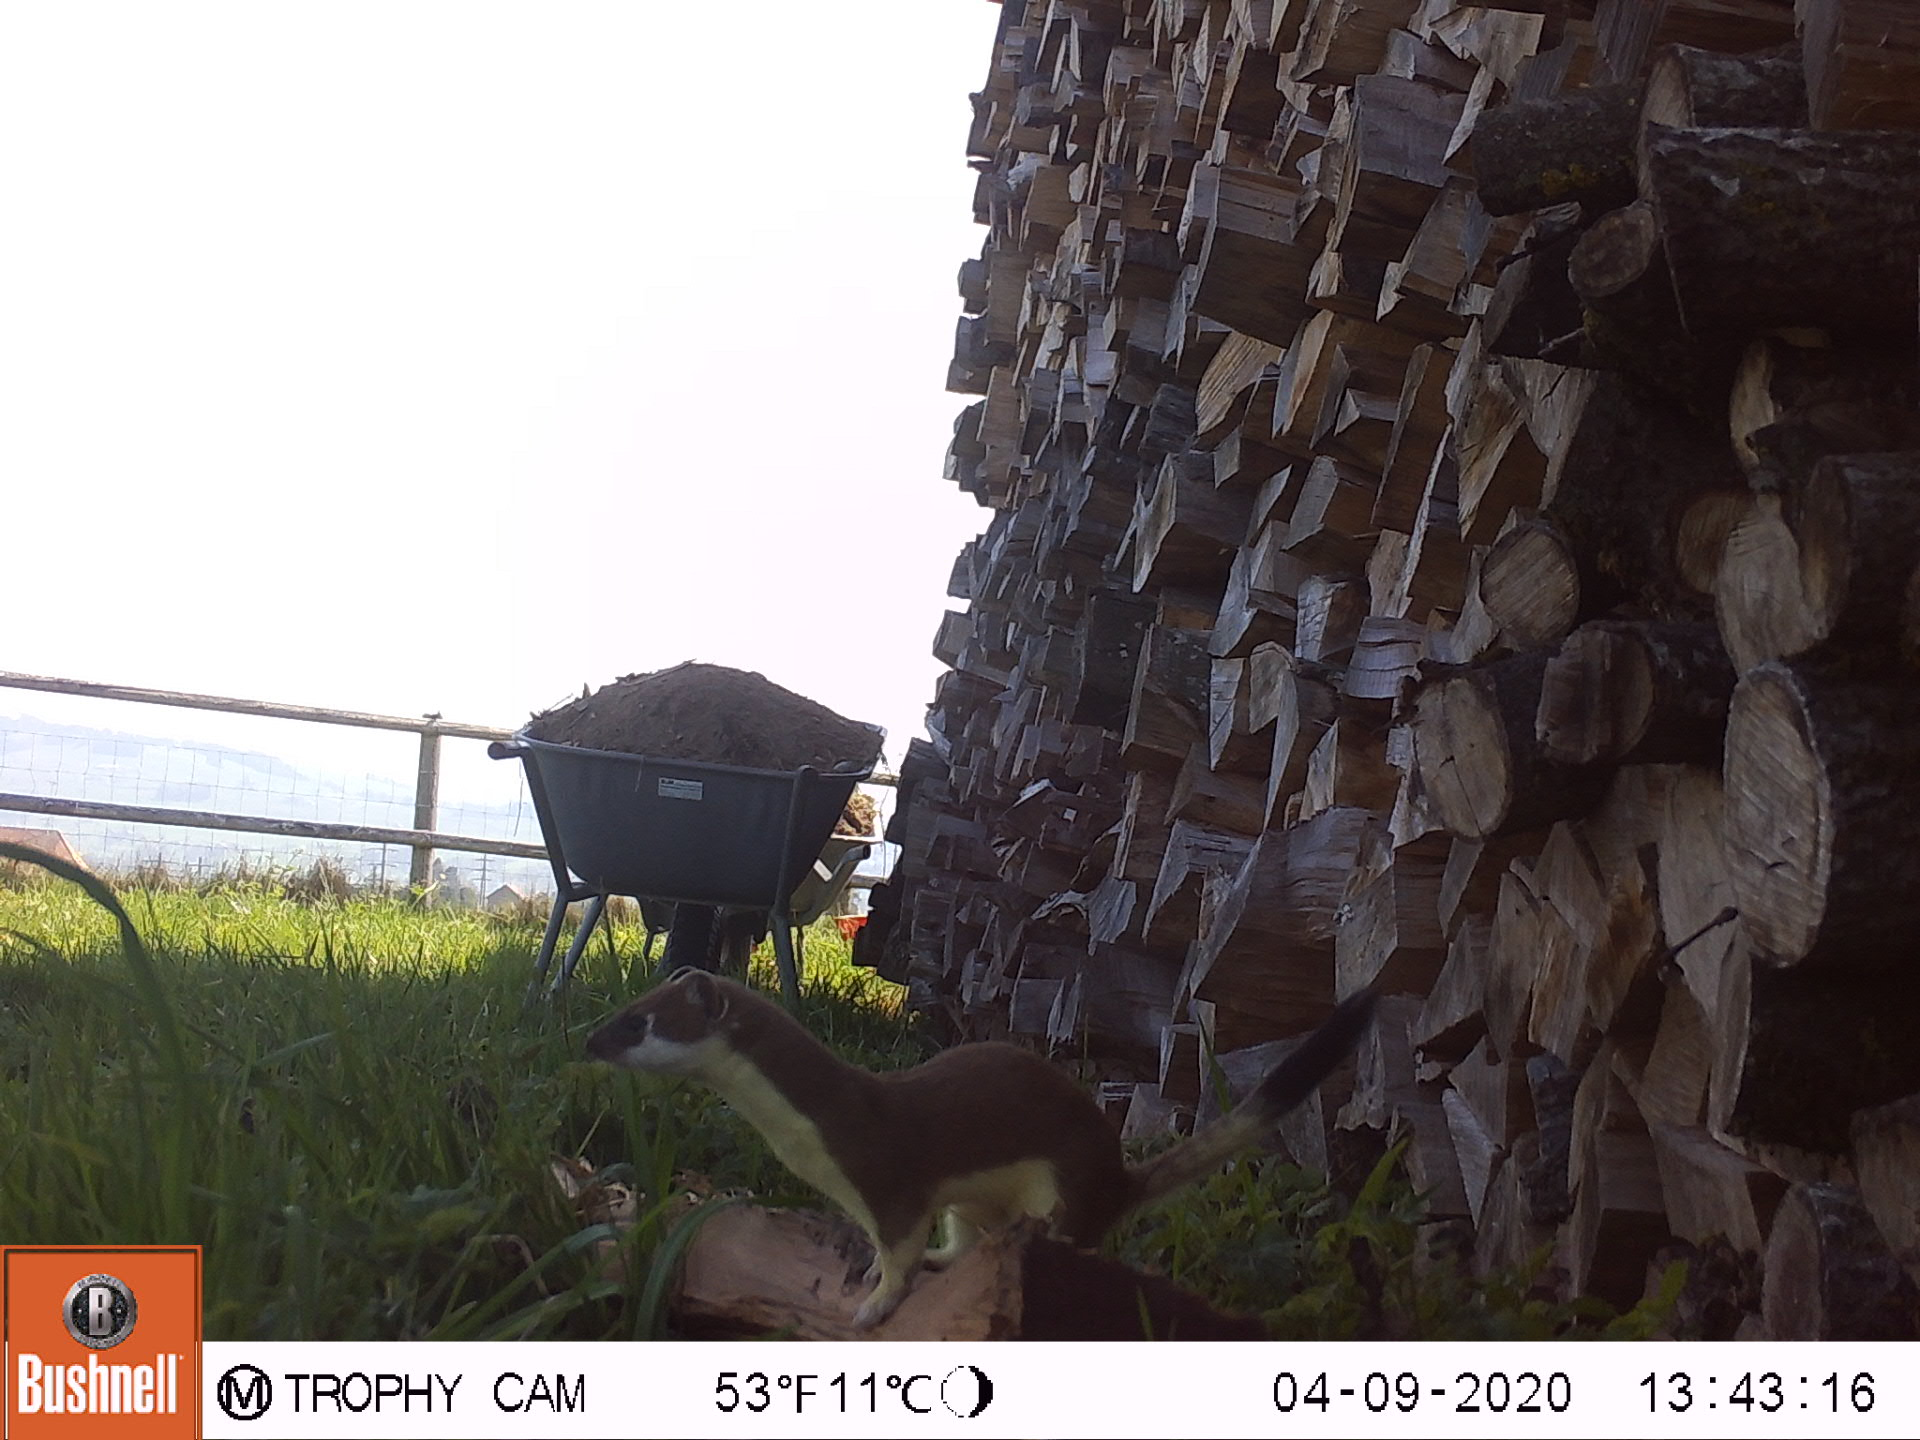
\includegraphics{images/Hermelin_Str116_WK02.JPG}

\vspace{10pt}

{\huge \@title}

\vspace{30pt}

% {\Large \@subtitle}
% 
% {\Large \@date}



\end{center}



\begin{flushleft}

% \begin{table}[]
\begin{minipage}{21cm}
\vspace{10cm}


\begin{tabular}{ll}
Auftraggeber: & \textbf{Wiesel \& Co am Zimmerberg}                         \\
              & c / o Stefan Keller                                         \\
              & Aeschstrasse 23,                                            \\
              & 9122 Mogelsberg                                             \\
              &                                                             \\
Bearbeitung:  & \textbf{Institut für Umwelt und Natürliche Ressourcen IUNR} \\
              & ZHAW Zürcher Hochschule für Angewandte Wissenschaften       \\
              & Life Sciences und Facility Management                       \\
              & Forschungsgruppe Geoinformatik                              \\
              & Grüental, Postfach                                          \\
              & CH-8820 Wädenswil                                           \\
              &                                                             \\
Autoren:      & Nils Ratnaweera\textsuperscript{1}                         \\
              & Inga Laas\textsuperscript{2}                              \\
              & Silvio Aegerter\textsuperscript{2}                        \\
              & Patrick Laube\textsuperscript{1}                           \\
              &                                                             \\
              & \textsuperscript{1} ZHAW, \textsuperscript{2} Wiesel \& Co am Zimmerberg \\
              &                                                             \\
              &                                                             \\
Titelbild:    & Hermelin vor einem Winterquartier (Laas, 2020)                
\end{tabular}
% \end{table}
\end{minipage}


\end{flushleft}

\end{titlepage}
\makeatother


\let\maketitle\oldmaketitle



{
\setcounter{tocdepth}{1}
\tableofcontents
}
\hypertarget{danksagung}{%
\chapter{Danksagung}\label{danksagung}}

Dieser Bericht ist durch die Mitwirkung vieler engagierter Personen entstanden, bei denen wir uns an dieser Stelle bedanken möchten:

\begin{itemize}
\tightlist
\item
  Simon Capt für seine fachlichen Einschätzungen sowie der Bestimmung und Gegenkontrolle von zahlreichen Spurenpapieren
\item
  Inga Laas und Silvio Aegerter für ihr grosses Engagement bei der Erhebung der Daten aus Spurentunneln und Fotofallen
\item
  Adrian Dietrich (SWILD), Andrin Dürst (Naturpark Thal) sowie Matthias Nyfeler (ZHAW) für ihre Inputs für die statistische Auswertung der Daten
\item
  Zahlreiche freiwilligen Helfer bei der Betreuung von Spurentunneln sowie die Meldung von Beobachtungen
\end{itemize}

\hypertarget{zusammenfassung}{%
\chapter*{Zusammenfassung}\label{zusammenfassung}}
\addcontentsline{toc}{chapter}{Zusammenfassung}

Im Projekt ``Wiesel \& Co am Zimmerberg'' werden die Tierarten Hermelin, Mauswiesel und Iltis mit gezielten Massnahmen gefördert. Dabei werden im Wesentlichen fünf Arten Typen von Aufwertungsmassnahmen umgesetzt: Winterquartiere, Ast- und Steinhaufen, Gebüschgruppen sowie Grossstrukturen. Von diesen Massnahmen sind bis heute über 450 realisiert worden.

Das Ziel der vorliegenden Wirkungskontrolle ist festzustellen, ob diese Aufwertungsmassnahmen von den Zielarten genutzt werden. Dafür wurden Ast- und Steinhaufen mit Spurentunnel und Winterquartieren mit Fotofallen systematisch beobachtet. Zudem wurden zur Beurteilung zwei weitere Datensätzen zugezogen, die im Rahmen des Naturschutz-Projekts erhoben wurden: Dabei handelt es sich die Resultate von spontanen Wirkungskontrollen sowie um Beobachtungsmeldungen aus der Bevölkerung.

In der \textbf{Spurentunnel Untersuchung} sind 39 Asthaufen innerhalb von zwei Jahren über einen Zeitraum von je 6 Wochen systematisch untersucht worden. Die Untersuchungen fanden im Herbst 2019 sowie im Frühling 2020 statt. Anhand der Spurenpapiere konnten über beide Perioden 55 Einzelnachweise vom Hermelin und zwei Einzelnachweise vom Iltis gemacht werden. Die dritte Zielart, das Mauswiesel, konnte an keinem Standort nachgewiesen werden. Über beide Untersuchungsperioden hinweg konnten in 27 von 39 Asthaufen (69 \%) mindestens eine Zielart detektiert werden

In der \textbf{Fotofallen-Überwachung} der Winterquartiere konnten in 5 von 11 untersuchten Standorten (45\%) mindestens eine Zielart festgestellt werden. Jedes Winterquartier wurde von Kleintieren genutzt: Von Dachsen, Eichhörnchen, Füchsen, Mardern, Fröschen, Vögeln, Mäusen und Hauskatzen.

In der unsystematischen, \textbf{spontanen Spurentunnel-Untersuchung} konnte in den insgesamt 32 beobachteten Asthaufen das Hermelin 51 und der Iltis 23-mal nachgewiesen werden. Auch in dieser Erhebung konnte das Mauswiesel nicht nachgewiesen werden. In 25 der 32 Asthaufen (78\%) konnte mindestens eine der Zielarten festgestellt werden.

Von den 555 \textbf{Sichtungsmeldungen} , die im Projekt gesammelt wurden, sind 428 Meldungen verwendbar. Diese zeigen, dass das Hermelin weitestgehend im ganzen Bezirk beobachtet werden konnte, so auch in stark fragmentierten und dicht besiedelten Kulturflächen. Deutliche Häufungen von Meldungen sind aber in den weniger verbauten Landschaften zu verzeichnen. Deutlich weniger Sichtungsmeldungen sind zum Iltis eingegangen. Dies wiederspiegelt einerseits die tiefere Anzahl Individuen im Vergleich zur Hermelinpopulation, ist aber mit Sicherheit auch der Lebensweise dieser Tierart geschuldet: Als dämmerungs- und nachtaktives Tier, welches sich auch gerne im Waldrandbereich aufhaltet, ist der Iltis seltener zu beobachten als das Hermelin.

Ebenfalls sind Beobachtungen von Mauswieseln sehr rar und über den ganzen Bezirk verteilt. Auch hier ist das ein Resultat von zwei verschiedenen Faktoren bestimmt: Das Mauswiesel ist sehr schwierig zu beobachten und zuverlässig von Hermelinen zu unterscheiden. Es kann aber zusätzlich davon ausgegangen werden, dass die Mauswieselpopulation im Bezirk eher klein und fragil ist.

\hypertarget{ausgangslage}{%
\chapter{Ausgangslage}\label{ausgangslage}}

Das Projekt ``Wiesel \& Co am Zimmerberg'' ist eine gemeinsame Aktion der Naturschutzvereine des Bezirks Horgen. Im Zentrum dieses Naturschutzprojekts steht die Förderung der Tierarten Hermelin, Mauswiesel und Iltis.

Zur Förderung dieser Zielarten werden in erster Linie ihre Lebensräume aufgewertet. Dazu werden natürliche Strukturen wie Asthaufen und Hecken geschaffen, um mehr Deckungsmöglichkeiten, grösseren Beuteerfolg und bessere Bedingungen für die Aufzucht von Jungen zu schaffen.

Konkret werden im Projekt Massnahmen gefördert, welche unter \href{https://wieselundco.ch/welche-massnahmen}{wieselundco.ch/welche-massnahmen} beschrieben sind. Im Projekt wird die Realisierung dieser Massnahmen beratend, tatkräftig und teilweise finanziell unterstützt. Die finanzielle Unterstützung erfolgt bei der Umsetzung folgender Massnahmen (siehe auch Abbildung \ref{fig:massnahmen}):

\begin{enumerate}
\def\labelenumi{\arabic{enumi}.}
\tightlist
\item
  Ast- / Steinhaufen
\item
  Winterquartiere
\item
  Gebüschgruppen
\item
  Grossstrukturen
\item
  Sanierung von Feldscheunen
\end{enumerate}

Von den etwa 450 Massnahmen, die im Rahmen des Naturschutzprojekts umgesetzt wurden, handelt es sich bei über 60 \% um Asthaufen. Etwa 20 \% der Massnahmen sind Gebüschgruppen und weitere 10 \% Steinhaufen. Winterquartiere und Grossstrukturen bilden die restlichen 10 \%.

Die vorliegende Wirkungskontrolle soll feststellen, ob die Aufwertungsmassnahmen für die Zielarten attraktiv sind und von ihnen genutzt werden. Dafür werden Ast- und Steinhaufen mit Spurentunnel und Winterquartiere mit Fotofallen systematisch beobachtet. Zudem werden zur Beurteilung zwei weitere Datensätze des Projekts beigezogen, die bereits vorliegen. Dabei handelt es sich um die Resultate von spontanen Wirkungskontrollen sowie um Beobachtungsmeldungen aus der Bevölkerung.



\begin{figure}[H]
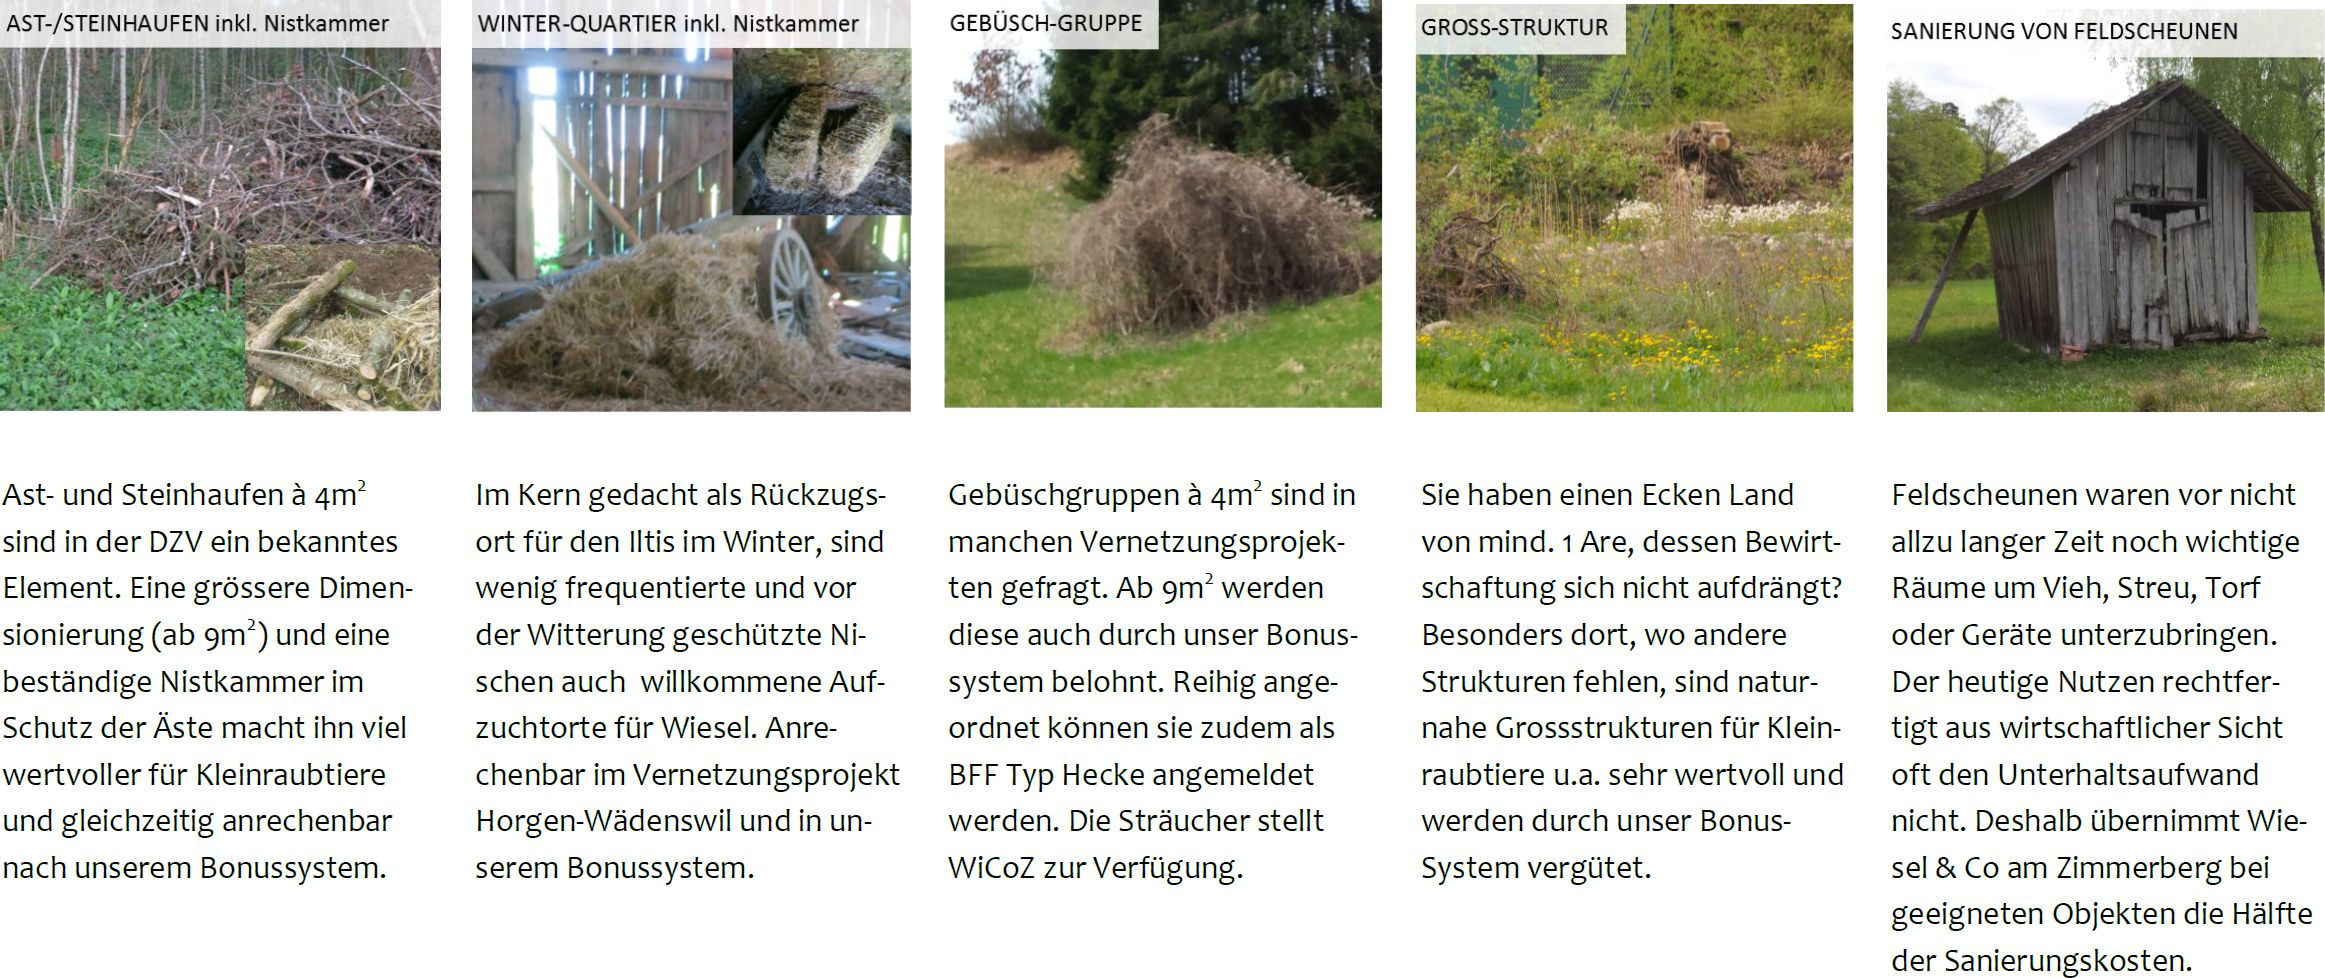
\includegraphics[width=1\linewidth]{images/massnahmen} \caption{Massnahmen, die im Projekt gefördert werden (Quelle: \href{http://www.wieselundco.ch/bonus}{wieselundco.ch/bonus})}\label{fig:massnahmen}
\end{figure}

\hypertarget{konzept-der-vorliegenden-wirkungskontrolle}{%
\chapter{Konzept der vorliegenden Wirkungskontrolle}\label{konzept-der-vorliegenden-wirkungskontrolle}}

Die vorliegende Wirkungskontrolle entspricht einer Synthese zwischen der Attraktivitätskontrolle ausgewählter Lebensraumaufwertungen und ergänzenden Datensätzen von Wiesel \& Co am Zimmerberg. Folgende Hintergründe erklären die Wahl des gewählten Konzepts:

Gemäss dem Konzept von Müri und Weinberger (2013) besteht die Erfolgskontrolle aus der Umsetzungskontrolle, der Attraktivitätskontrolle sowie der Populationskontrolle. Diese Bestandteile können auch als drei unterschiedliche Ansätze verstanden werden, um den Erfolg eines Aufwertungsprojektes zu messen, und unterscheiden sich stark in ihrem Aufwand und ihrer Aussagekraft.

Die \textbf{Umsetzungskontrolle} stellt die einfachste Art dar, den Erfolg des Projektes zu messen. Dabei gilt es die Anzahl der realisierten Massnahmen bzw. deren Anteil an den geplanten Massnahmen zu bestimmen. Dieser Kennwert (z.B. ``80\% aller geplanten Massnahmen konnten umgesetzt werden'') sagt jedoch wenig darüber aus, ob die umgesetzten Massnahmen auch zum gewünschten Erfolg (Stärkung der lokalen Wieselpopulation) beitragen. Werden Massnahmen ungünstig angelegt, sind sie für die Zielarten nicht nutzbar. Die Umsetzungskontrolle erfolgt in den Berichterstattungen, welche einsehbar sind unter: \href{http://www.wieselundco.ch/projekt/resultate}{wieselundco.ch/projekt/resultate}.

Am aufwändigsten ist die \textbf{Populationskontrolle} : Hier wird untersucht, ob sich die Population durch die umgesetzten Massnahmen günstig entwickelt hat. Eine solche Untersuchung hat die grösste Aussagekraft, da sie direkt die Kernfrage beantwortet. Jedoch unterliegen Hermelin- und Mauswieselpopulationen starken Schwankungen, die von externen Faktoren wie Witterung und Nahrungsverfügbarkeit abhängig sind. Um eine fundierte Aussage über die projektbedingte Populationsentwicklung machen zu können, wären Langzeitstudien vor und nach der Umsetzung nötig, was finanziell und logistisch einen unverhältnismässig hohen Aufwand bedeuten würde.

Bei der \textbf{Attraktivitätskontrolle} handelt es sich um einen Kompromiss zwischen Machbarkeit und Aussagekraft. Diese fokussiert auf die Frage, ob und wie häufig die erstellten Strukturen von den Zielarten genutzt wurden. Sie hat eine erheblich grössere Aussagekraft als diejenige der Umsetzungskontrolle, weil die Nutzung der Strukturen mitberücksichtigt wird. Die vorliegende Untersuchung verfolgt diesen Ansatz (``Attraktivitätskontrolle''). Dazu wurden zwei Erhebungen durchgeführt: Zum einen wurden \textbf{Asthaufen mit Spurentunnel} , zum anderen \textbf{Winterquartiere mit Fotofallen} beobachtet.

Die Resultate der Spurentunnel und Fotofallen geben nicht nur Aufschluss darüber, wie viele sondern auch welche Strukturen wie oft (und von welchen Arten) besucht wurden. Eine Erhebung verschiedener Parameter von sehr gut und sehr schlecht frequentierten Asthaufen soll Aufschlüsse über die Faktoren geben, was Strukturen für Wiesel \& Co attraktiv machen.

Zusätzlich werden zwei weitere Datensätze von Seite Wiesel \& Co am Zimmerberg beigezogen: Zum einen handelt es sich um Daten von spontan und unsystematisch durchgeführten Spurentunnel Erhebungen und zum anderen um Sichtungsmeldungen aus der Bevölkerung. Weitere Details dazu im nächsten Kapitel ``Methode''.

\hypertarget{methode}{%
\chapter{Methode}\label{methode}}

\hypertarget{uxfcbersicht}{%
\section{Übersicht}\label{uxfcbersicht}}

Die Attraktivitätskontrolle besteht aus der Beobachtung zweier verschiedener Massnahmentypen in jeweils zwei Zeitperioden. Ergänzend dazu liegen zwei Datensätze vor, die während der Projektdauer unter Einbezug von interessierten Laien erzeugt wurden (sogenannte Bürgerwissenschaften). Diese Erhebungen und Datensätze werden nachstehend beschrieben und sind in Tabelle \ref{tab:erhebungswochen} zusammengefasst.

Bei \textbf{Erhebung 1} handelt es sich um eine systematische Kontrolle ausgewählter Asthaufen während zweier Jahre (2019 / 2020) über einen definierten Zeitraum. Diese Erhebungen wurden nach einheitlicher Vorgehensweise durchgeführt. Im gleichen Zeitraum wurden in \textbf{Erhebung 2} sogenannte Winterquartiere (siehe \href{http://www.wieselundco.ch/bonus}{wieselundco.ch/bonus}), ebenfalls systematisch beobachtet. \textbf{Erhebung 3} ist eine Aufnahme und Beurteilung von 9 verschiedenen Merkmale von sehr gut sowie sehr schlecht besuchten Asthaufen.

Bei \textbf{Datensatz A} handelt es sich um die Resultate von spontan durchgeführten Kontrollen einzelner Asthaufen und Grossstrukturen mit Fotofallen und / oder Spurentunneln. Diese Kontrollen dienten unter anderem auch dazu, Freiwilligen, Naturschutzvereins-Mitgliedern sowie Schüler*innen einen tieferen Einblick in das Projekt und dessen Ziele zu geben. Bei \textbf{Datensatz B} handelt es sich um Sichtungsmeldungen aus der Bevölkerung, die seit Projektbeginn über ein Onlinetool erfasst werden (\href{http://www.wieselundco.ch/beobachtung}{wieselundco.ch/sichtungskarte}).

\begin{table}

\caption{\label{tab:erhebungswochen}Zusammenfassung der Ansätze, die für die Datenbeschaffung verfolgt wurden.}
\centering
\begin{tabular}[t]{llp{20mm}lp{22mm}p{40mm}}
\toprule
Bezeichnung & Strukturen & Zeitraum & Dauer & Methode & Anzahl\\
\midrule
\cellcolor{gray!6}{Erhebung 1} & \cellcolor{gray!6}{Asthaufen} & \cellcolor{gray!6}{Herbst ’19 / Frühling ‘20} & \cellcolor{gray!6}{6 Wochen} & \cellcolor{gray!6}{Spurentunnel} & \cellcolor{gray!6}{39 Asthaufen}\\
Erhebung 2 & Winterquartiere & Herbst ’19 / Frühling ‘20 & 6 Wochen & Fotofallen & 11 Winterquartiere\\
\cellcolor{gray!6}{Datensatz A} & \cellcolor{gray!6}{Asthaufen} & \cellcolor{gray!6}{2014 - 2019} & \cellcolor{gray!6}{Variabel} & \cellcolor{gray!6}{Spurentunnel / Fotofallen} & \cellcolor{gray!6}{32 Asthaufen}\\
Datensatz B & Keine & 2014 – dato & laufend & Beobachtungs-meldungen & > 500 Einzelbeobachtungen\\
\bottomrule
\end{tabular}
\end{table}



\begin{figure}
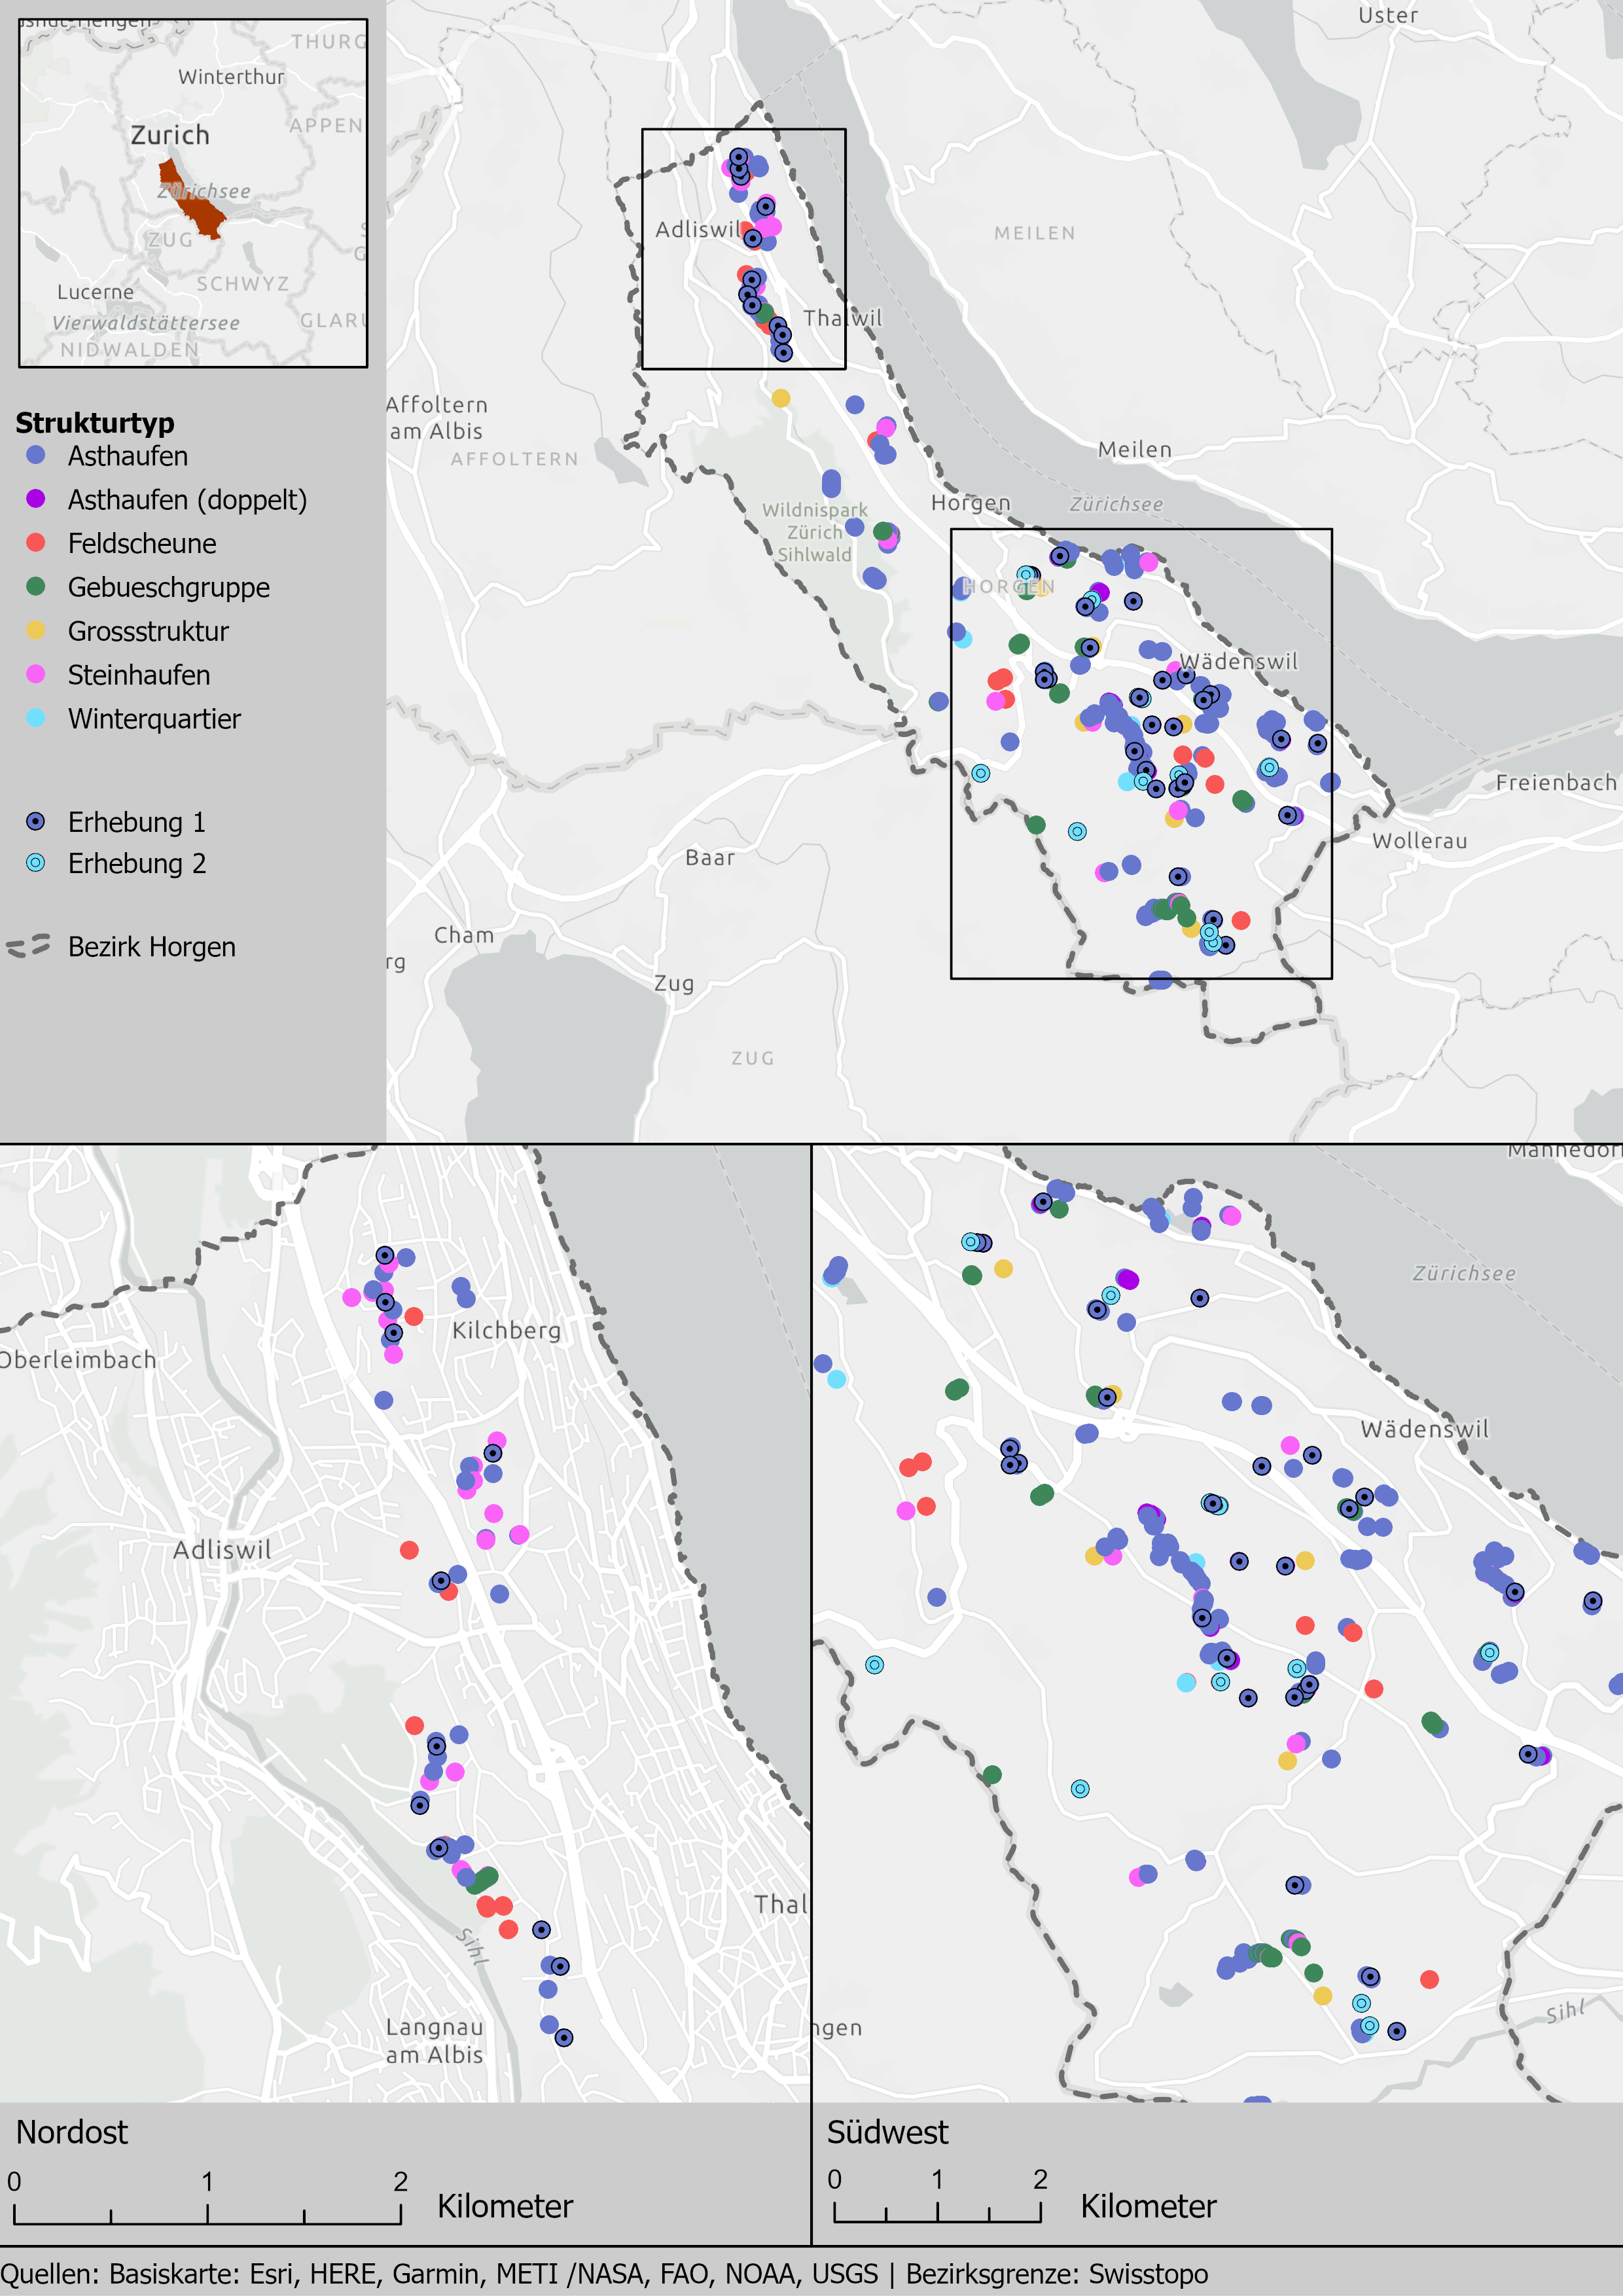
\includegraphics[width=1\linewidth]{images/Layout_Strukturen} \caption{Perimeter des Projekts Wiesel und Co am Zimmerberg sowie der umgesetzten Massnahmen während der Projektdauer (Total ca. 450 Strukturen). Die untersuchten Asthaufen und Winterquartiere aus Erhebung 1 und 2 sind farblich markiert.}\label{fig:layoutstrukturen}
\end{figure}

\hypertarget{erhebung-1-attraktivituxe4tskontrolle-von-asthaufen-mittels-spurentunneln}{%
\section{Erhebung 1: Attraktivitätskontrolle von Asthaufen mittels Spurentunneln}\label{erhebung-1-attraktivituxe4tskontrolle-von-asthaufen-mittels-spurentunneln}}

In diesem Ansatz sind 39 Asthaufen in zwei Jahren über einen Zeitraum von je 6 Wochen systematisch mit Spurentunneln untersucht worden. Die Untersuchungen fanden im Herbst 2019 sowie im Frühling 2020 statt (nähere Angaben siehe Abbildung \ref{fig:erhebungswoche}). Details zu dieser Erhebungsmethode können aus King et al.~(1977) entnommen werden.

Von den 39 beobachteten Asthaufen liegen 11 im Nordwesten (Gemeinde Kilchberg) und 28 im Südosten (Gemeinde Wädenswil) des Bezirks Horgen (siehe Abbildung \ref{fig:layoutstrukturen}). Bei der Standortwahl wurde darauf geachtet, dass sie in der jeweiligen Region möglichst gut auf die Gesamtheit aller Standorte verteilt wurden. Ausserdem wurden Standorte bevorzugt, die wenig begangen werden, um das Risiko von Fremdmanipulationen zu reduzieren.

Die Kontrollen fanden wöchentlich und nach einheitlichem Schema statt (nach Anleitung von Müri et al., 2015). Die Spurentunnel wurden nach Möglichkeit mit der Öffnung von der Wetterseite abgewendet, um die Tinte der Witterung weniger auszusetzen. Zudem wurde bei Asthaufen an Wald- oder Heckenrändern die Tunnelöffnung immer zum Offenland ausgerichtet. Die Tintenkissen der Spurentunnel wurden beim Ausbringen der Tunnel getränkt und es wurde während der Dauer des Monitorings nach Bedarf Tinte nachgefüllt. Dabei wurden jeweils auch die Spurenpapiere ausgewechselt und die Struktur-ID, das Einlage- und Entnahmedatum, sowie die Laufrichtung notiert.

Um die Artbestimmung der erfassten Spuren sicherzustellen, erfolgte die Auswertung der Spurenpapiere durch Simon Capt vom CSCF, der viel Erfahrung in der Interpretation von Trittsiegeln besitzt (u.a. nationales Mustelidenmonitoring, Capt et al, 2010). Die Analyse der Resultate beschränkt sich auf die Zielarten Hermelin, Mauswiesel und Iltis.



\begin{figure}
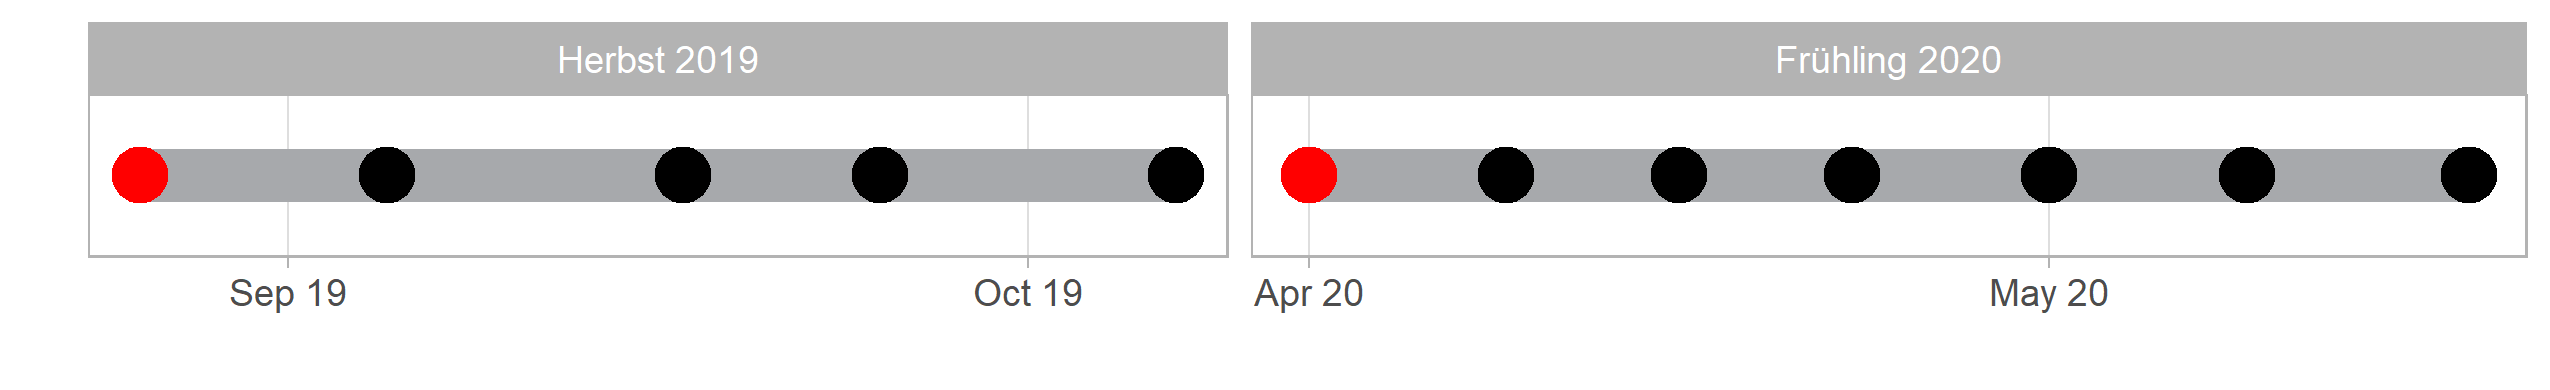
\includegraphics[width=1\linewidth]{images/Erhebungswochen} \caption{Visualisierung der Kontrollphase der beiden Erhebungsperioden. Der rote Punkt markiert das Ausbringen der Spurentunnel, die schwarzen Punkte stellen jeweils die Daten dar, an denen die Spurenpapiere ausgetauscht wurden. Aus logistischen Gründen wurden im Herbst 2019 nur 4 Kontrollgänge durchgeführt, was sich jedoch nicht auf die Resultate auswirken sollte.}\label{fig:erhebungswoche}
\end{figure}

\hypertarget{erhebung-2-attraktivituxe4tskontrolle-von-winterquartieren-mittels-fotofallen}{%
\section{Erhebung 2: Attraktivitätskontrolle von Winterquartieren mittels Fotofallen}\label{erhebung-2-attraktivituxe4tskontrolle-von-winterquartieren-mittels-fotofallen}}

Die Überwachung der Winterquartiere wurde während sechs Wochen zwischen dem 26.08.2019 und 06.10.2019 sowie zwischen dem 30.3.2020 und 10.04.2020 durchgeführt. Untersucht wurden 11 Winterquartiere (alle in der Region Südost, siehe Abbildung \ref{fig:layoutstrukturen}).

Zur Untersuchung der Winterquartiere wurden Fotofallen mit Infrarotblitz von Bushnell verwendet. Als Setup wurde pro Auslösung ein Foto, sowie ein Film von 5 bis 10 Sekunden aufgenommen. Die Kameras wurden an einem eigens dafür eingeschlagenen Pfosten montiert, ergänzt mit einem Informationsblatt für Passanten.

Zur Auswertung der Bild- und Videoaufnahmen wurden sämtliche Dateien einzeln durchgeschaut und alle gefundenen Tiergruppen (ausser Mäusen und Katzen) aufaddiert. Die nachfolgende Analyse der Zahlen beschränkt sich jedoch auf die Zielarten.

\hypertarget{erhebung-3-erhebung-von-asthaufen-eigenschaften-zur-ermittlung-attraktivituxe4tsfuxf6rdernder-faktoren}{%
\section{Erhebung 3: Erhebung von Asthaufen Eigenschaften zur Ermittlung attraktivitätsfördernder Faktoren}\label{erhebung-3-erhebung-von-asthaufen-eigenschaften-zur-ermittlung-attraktivituxe4tsfuxf6rdernder-faktoren}}

Es ist anzunehmen, dass die Nutzung von Kleinstrukturen durch Kleinraubtiere von gewissen Faktoren besonders stark beeinflusst wird.
Um diese Annahme zu überprüfen wurden gemäss Erhebung 1, die 13 bestfrequentierten Asthaufen und 12 nicht frequentierte Asthaufen ausgewählt und im Feld aufgesucht. Jeder der 25 verschiedenen Asthaufen wurde auf 9 mutmasslich attraktivitätsbestimmende Faktoren untersucht und pro Faktor in eine von 5 Klassen eingeteilt (siehe nachstehende Tabelle).

\begin{table}

\caption{\label{tab:unnamed-chunk-3}Merkmalsausprägung pro untersuchtes Kriterium.}
\centering
\begin{tabular}[t]{l|l|l|l|l|l}
\hline
Merkmal & 0 & 1 & 2 & 3 & 4\\
\hline
Astmaterial & s. fein & fein & mittel & grob & s. grob\\
\hline
Volumen & s. klein & klein & mittel & gross & s. gross\\
\hline
Störung & s. gross & gross & mittel & klein & s. klein\\
\hline
Beuteangebot & s. klein & klein & mittel & gross & s. gross\\
\hline
Katzen & s. viel & viel & mittel & wenig & s. wenig\\
\hline
Andere Feinde & s. viel & viel & mittel & wenig & s. wenig\\
\hline
Benachbarte Kleinstrukturen & s. wenig & wenig & mittel & viel & s. viel\\
\hline
Benachbarte Korridore / Habitate & s. ungünstig & ungünstig & mittel & günstig & s. günstig\\
\hline
Pflege Aufstockung & s. schlecht & schlecht & mittel & gut & s. gut\\
\hline
\end{tabular}
\end{table}

Es ist zu beachten, dass fast alle Parameter keine exakt abgrenzbaren Klassengrenzen aufweisen. Die Erhebung kommt bei bei gewissen Parametern einer Schätzung gleich und die Beurteilung erfolgte aufgrund von Indizien: Die Nähe zu Wanderrouten (``Störung'') oder Siedlungen (``Katzen''), die Sichtung von Maushaufen (``Beuteangebot'') oder die Lebensraumqualität für grössere Prädatoren (``andere Fressfeinde'').
Andere Faktoren können hingegen klarer beurteilt werden, wie zum Beispiel das Volumen oder das Astmaterial (grob \ref{fig:astmaterial} links bzw. fein \ref{fig:astmaterial} rechts).

\begin{figure}
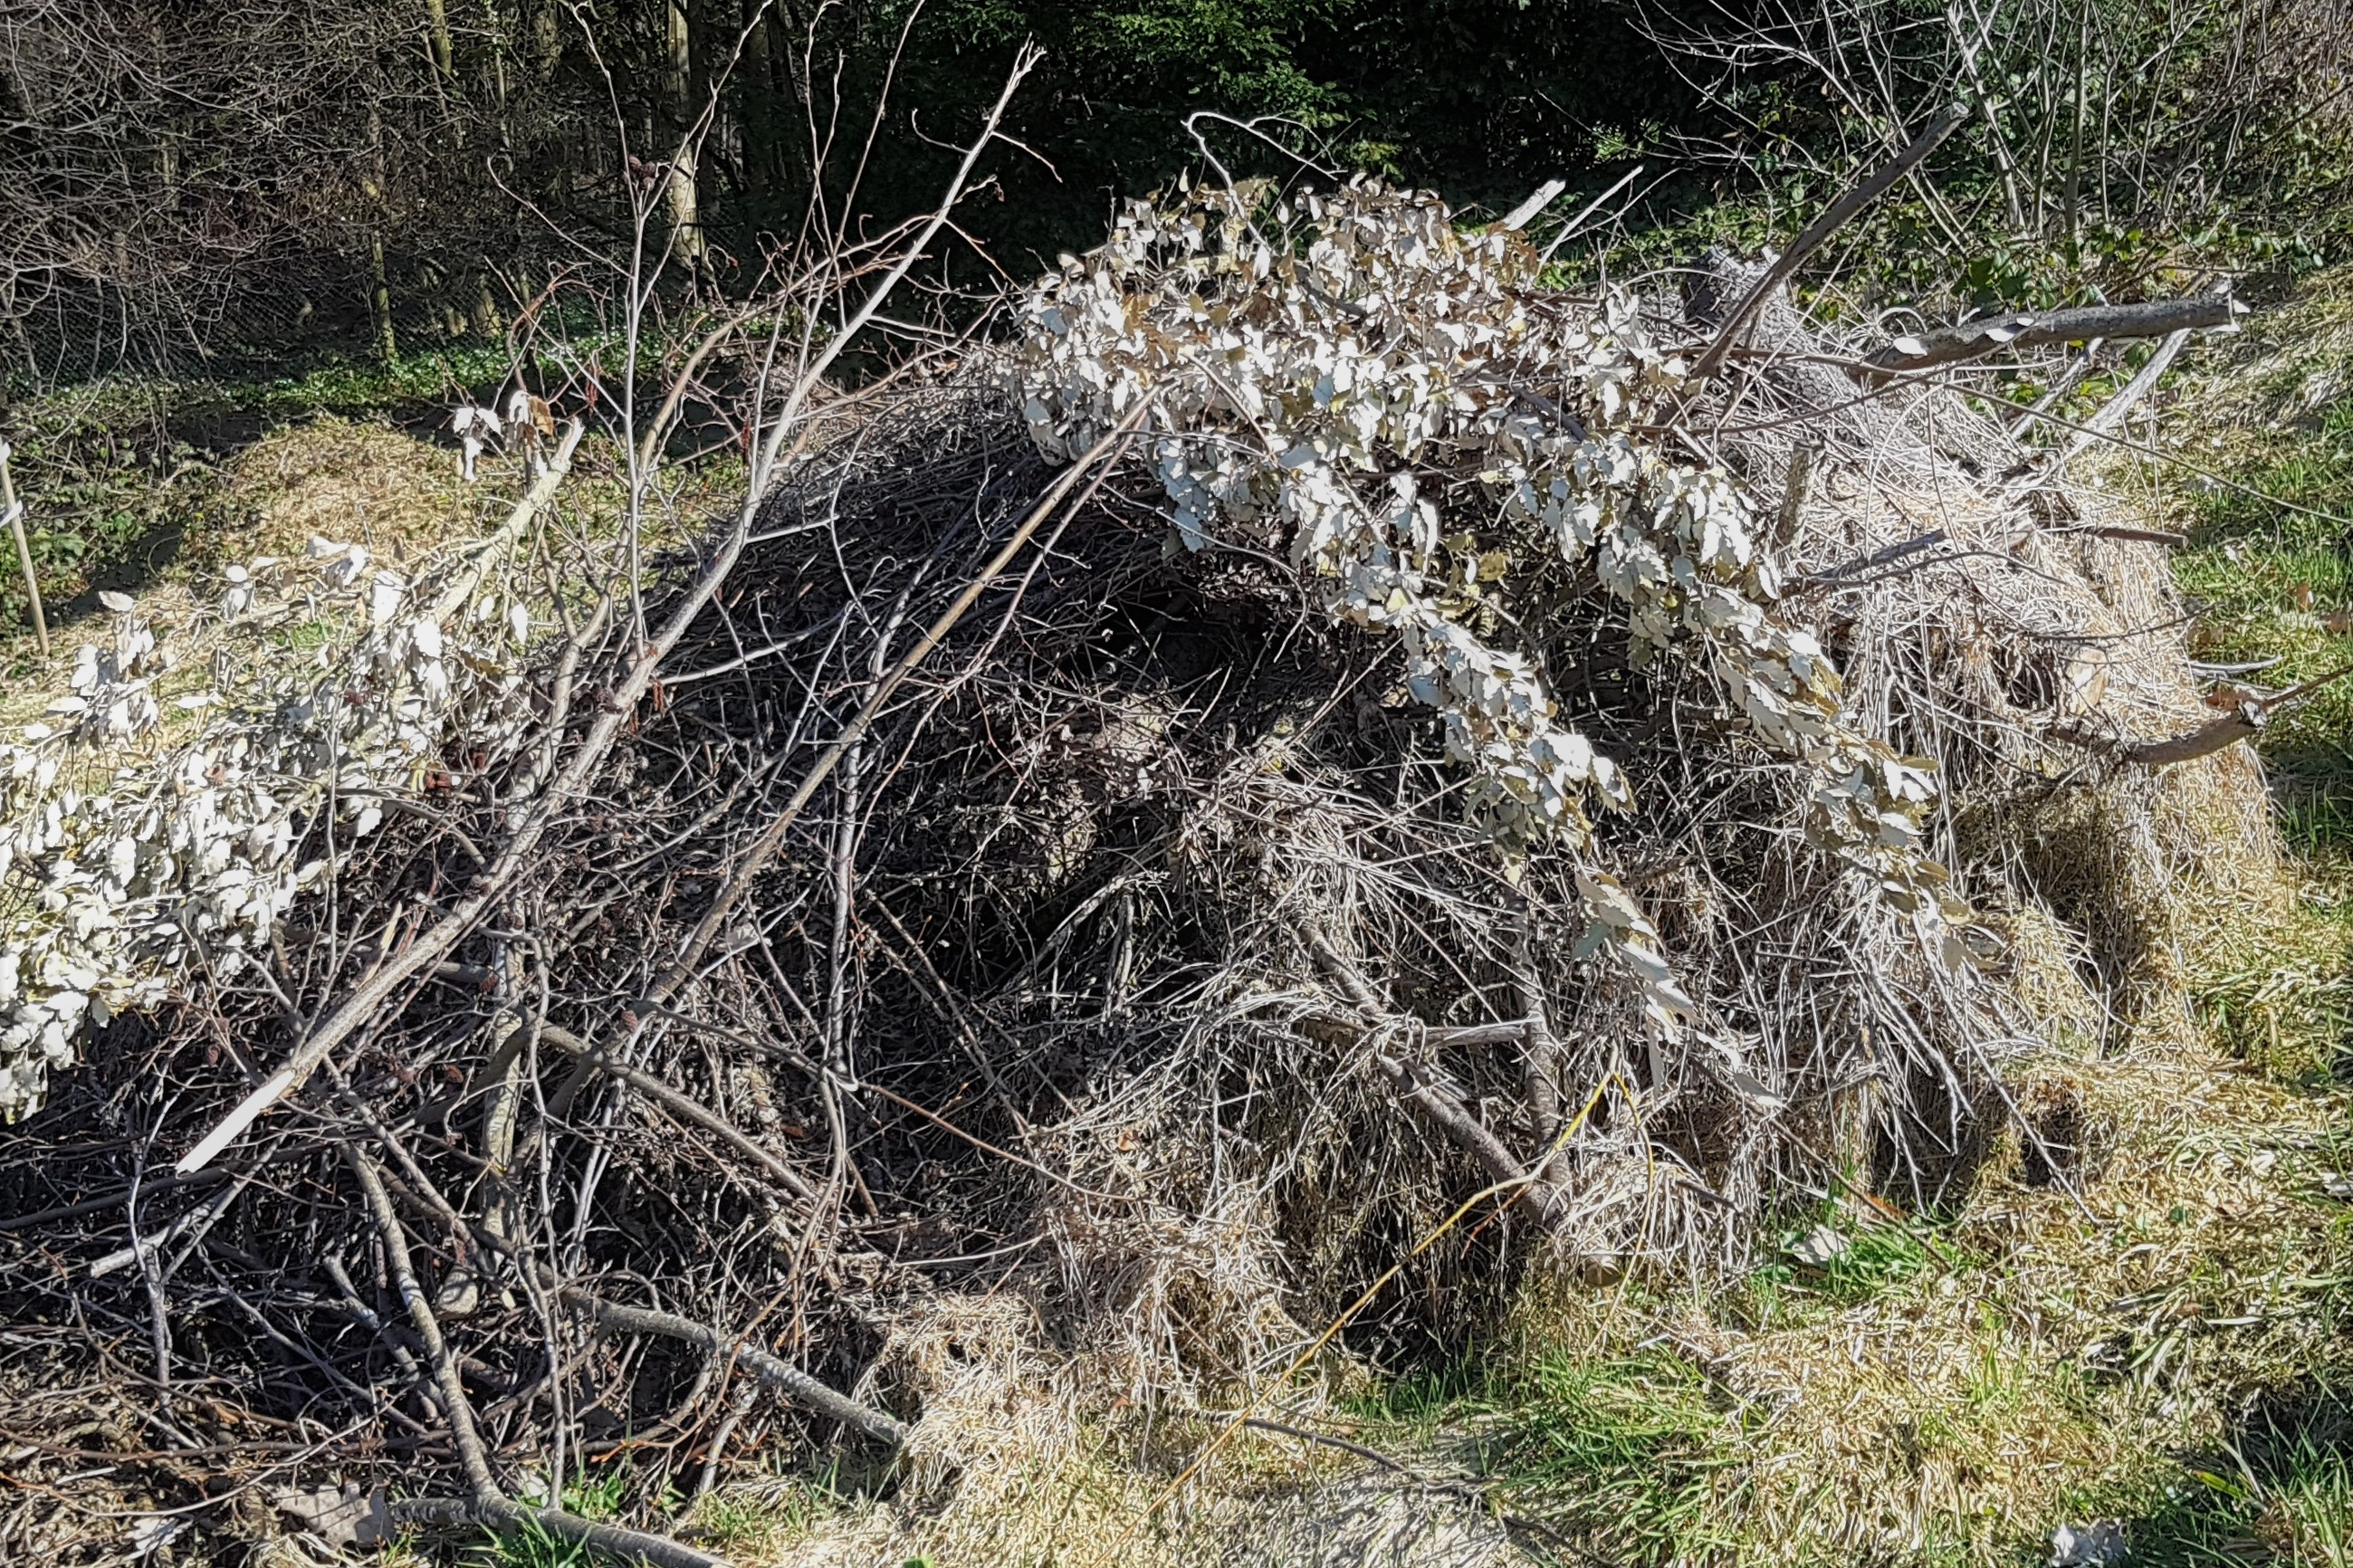
\includegraphics[width=0.49\linewidth]{images/feines_astmaterial} \caption{Zwei Asthaufen mit unterschiedlichem Material: Grob (links) bzw. fein (rechts)}\label{fig:astmaterial-1}
\end{figure}
\begin{figure}
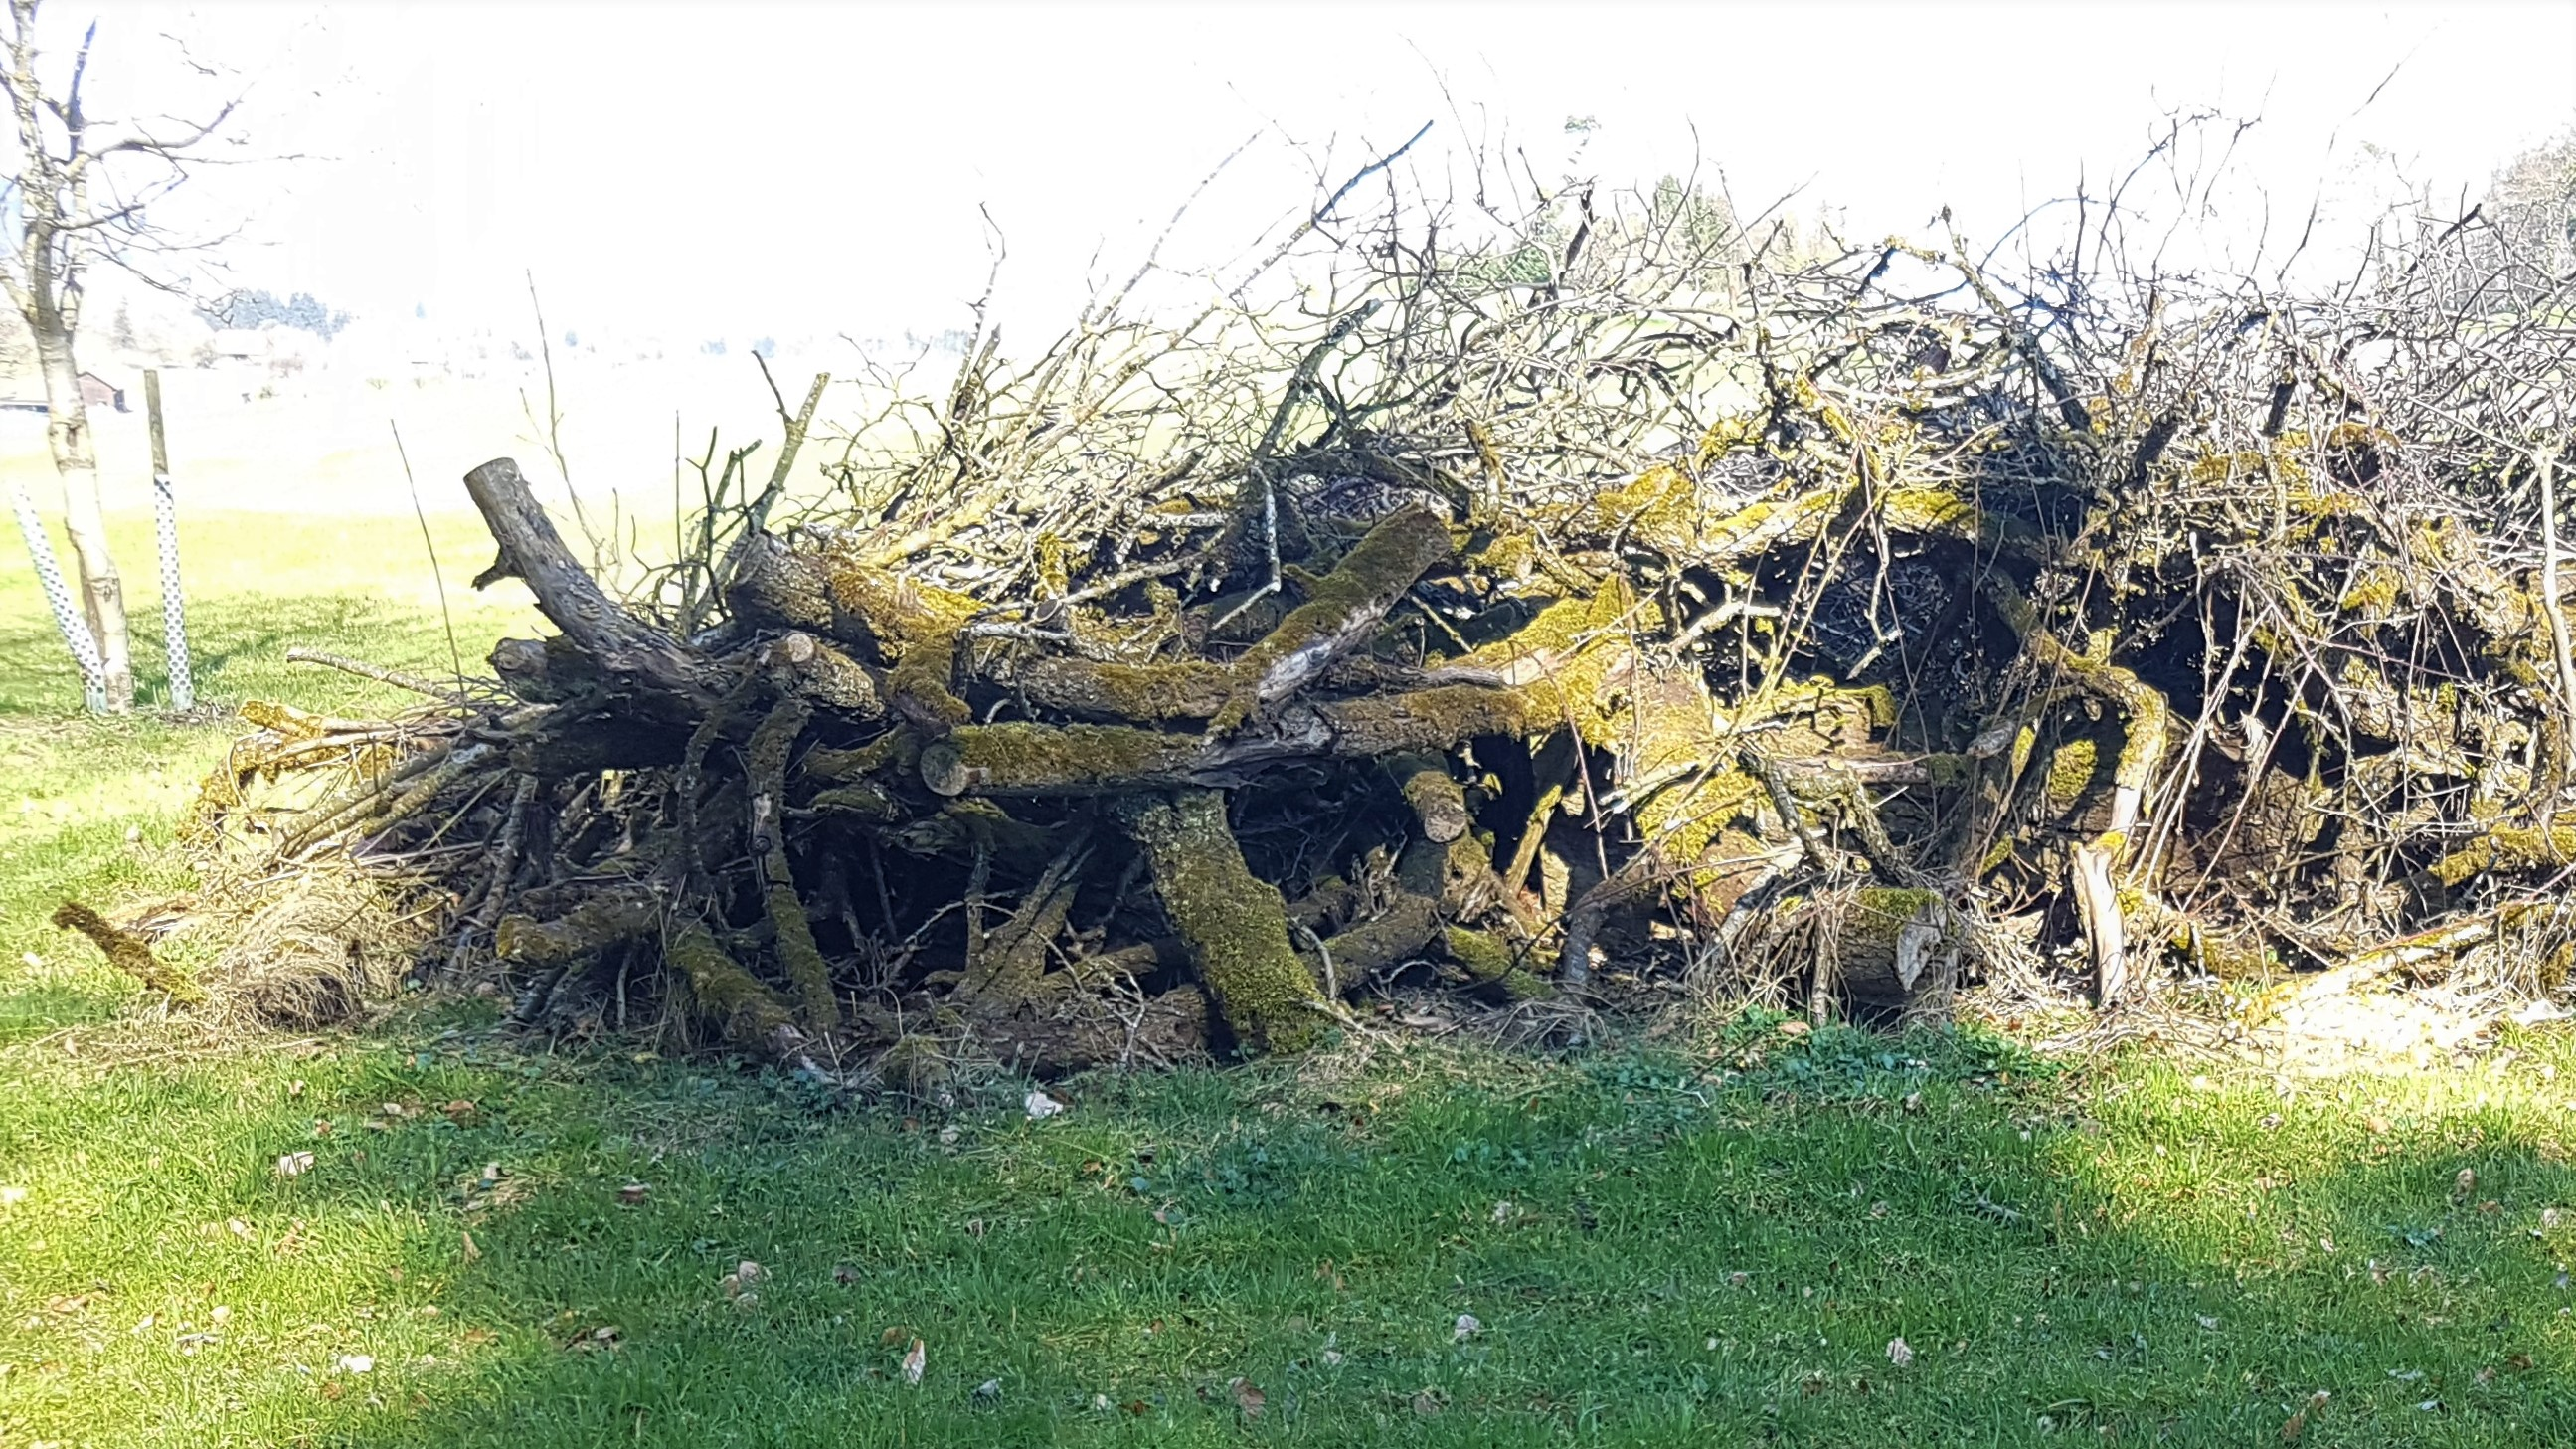
\includegraphics[width=0.49\linewidth]{images/grobes_astmaterial} \caption{Zwei Asthaufen mit unterschiedlichem Material: Grob (links) bzw. fein (rechts)}\label{fig:astmaterial-2}
\end{figure}

\hypertarget{datensatz-a-unsystematische-attraktivituxe4tskontrolle-von-asthaufen}{%
\section{Datensatz A: Unsystematische Attraktivitätskontrolle von Asthaufen}\label{datensatz-a-unsystematische-attraktivituxe4tskontrolle-von-asthaufen}}

Im Datensatz werden alle 32 Asthaufen berücksichtigt, die unmittelbar nach der Erstellung im Rahmen von Aktionstagen mit Spurentunnel ausgestattet und über einen variablen Zeitraum kontrolliert wurden (siehe Anhang C @ref(\#anhang-datensatz-a)). In ca. 50\% der Erhebungen wurden ergänzend Fotofallen eingesetzt. Die Erhebung dauerte in der Regel deutlich länger als 6 Wochen (höhere Detektionswahrscheinlichkeit), die Kontrollintervalle waren oft grösser als 2 Wochen (vermehrter Datenausfall). Die Beobachtung der Asthaufen verteilt sich über die Jahre 2014 bis 2019, wobei es 2016 zu einer Häufung kam. Es kam zu allen Jahreszeiten zu Kontrollaktivitäten, vermehrt im Frühling. Folgende Faktoren erschweren die Verwendung dieser Daten für einen Zielvergleich:

\begin{itemize}
\tightlist
\item
  die Kontrollen in der Kontrollphase (Dauer und Regelmässigkeit) wurden nicht einheitlich durchgeführt
\item
  leere Spurenpapiere wurden nicht systematisch dokumentiert. Es ist nicht genau nachvollziehbar, wie intensiv eine Struktur beobachtet wurde. Der Nachweiserfolg kann somit nicht in den Kontext des Nachweisefforts gesetzt werden.
\item
  die Auswahl der Standorte erfolgte vor allem aus praktischen Überlegungen (z.B. Interesse der Teilnehmenden an Aktionstagen)
\end{itemize}

Da der Datensatz mit beachtlichem Aufwand erhoben wurde, wird er in den vorliegenden Bericht integriert. Abbildung \ref{fig:wirkungskontrollespontaneffort} zeigt, für welche Kalenderwochen in welchen Jahren für eine Struktur ein Spurenpapier vorhanden ist. Dabei stellt jedes Quadrat eine Kalenderwoche einer Struktur dar und ist gelb eingefärbt, wenn ein Spurenpapier für diesen Zeitraum vorhanden ist.



\begin{figure}
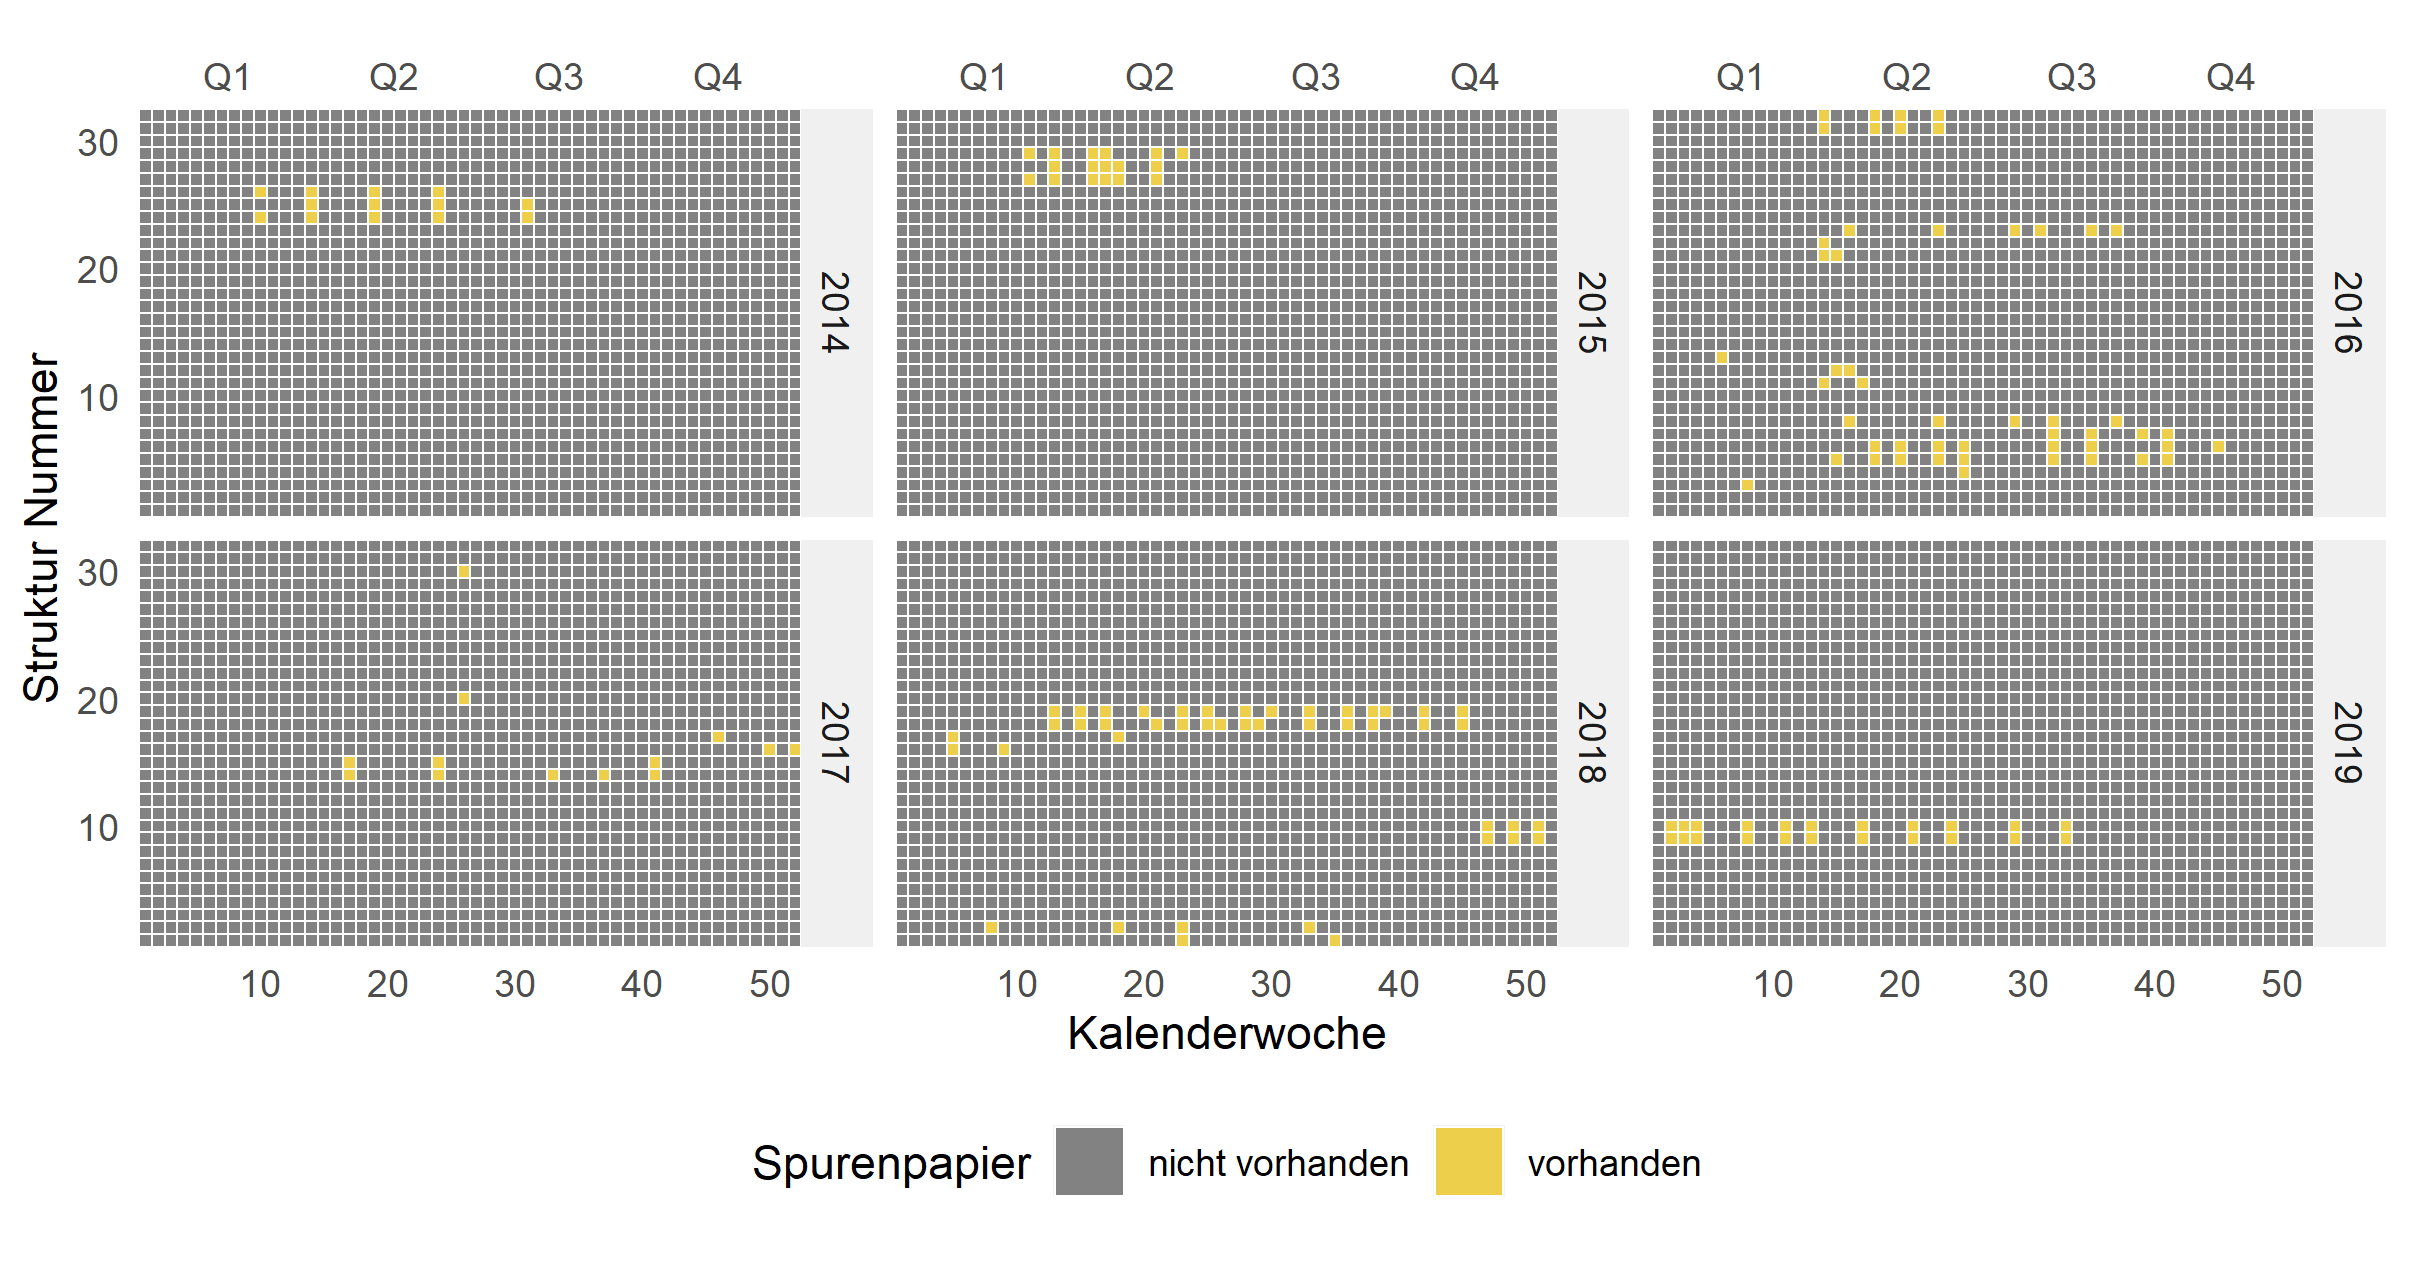
\includegraphics[width=1\linewidth]{images/wirkungskontrolle_spontan_effort} \caption{Visualisierung der fortlaufend kontrollierten Asthaufen (nach Ansatz 1). Jedes Quadrat stellt eine Kalenderwoche aus einem Jahr einer Struktur dar. Das Quadrat ist gelb eingefärbt, wenn in der entsprechenden Kalenderwoche ein Spurenpapier vorhanden ist und grau, wenn keines vorhanden ist.}\label{fig:wirkungskontrollespontaneffort}
\end{figure}

\hypertarget{methode-datensatz-b}{%
\section{Datensatz B: Beobachtungsmeldungen}\label{methode-datensatz-b}}

Seit Anbeginn des Projekts wurde die örtliche Bevölkerung dazu aufgerufen, Beobachtungen von Kleinraubtieren über das eigens dafür eingerichtete Webtool zu melden. Meldungen wurden auch via einen Flyer sowie per Mail oder auch mündlich aufgenommen. Beobachtungsmeldungen wurden durch den Projektleiter (Stefan Keller) verifiziert und in ``unsicher'', ``plausibel'' sowie ``sicher'' eingeteilt.

Auf diese Weise sind über 500 Meldungen zusammengetragen worden. Alle Meldungen, die über andere Kanäle als das Webtool erfasst wurden, sind vom Projektleiter gesammelt und periodisch in die Datenbank integriert worden. Diese erhielten als ``Erfassungsdatum'' jeweils das Datum dieser Überführung in die Datenbank, so sind im zeitlichen Verlauf der Meldungen deutliche Spitzen erkennbar (siehe Abbildung \ref{fig:beobachtungsmeldungenhistogramm}).



\begin{figure}
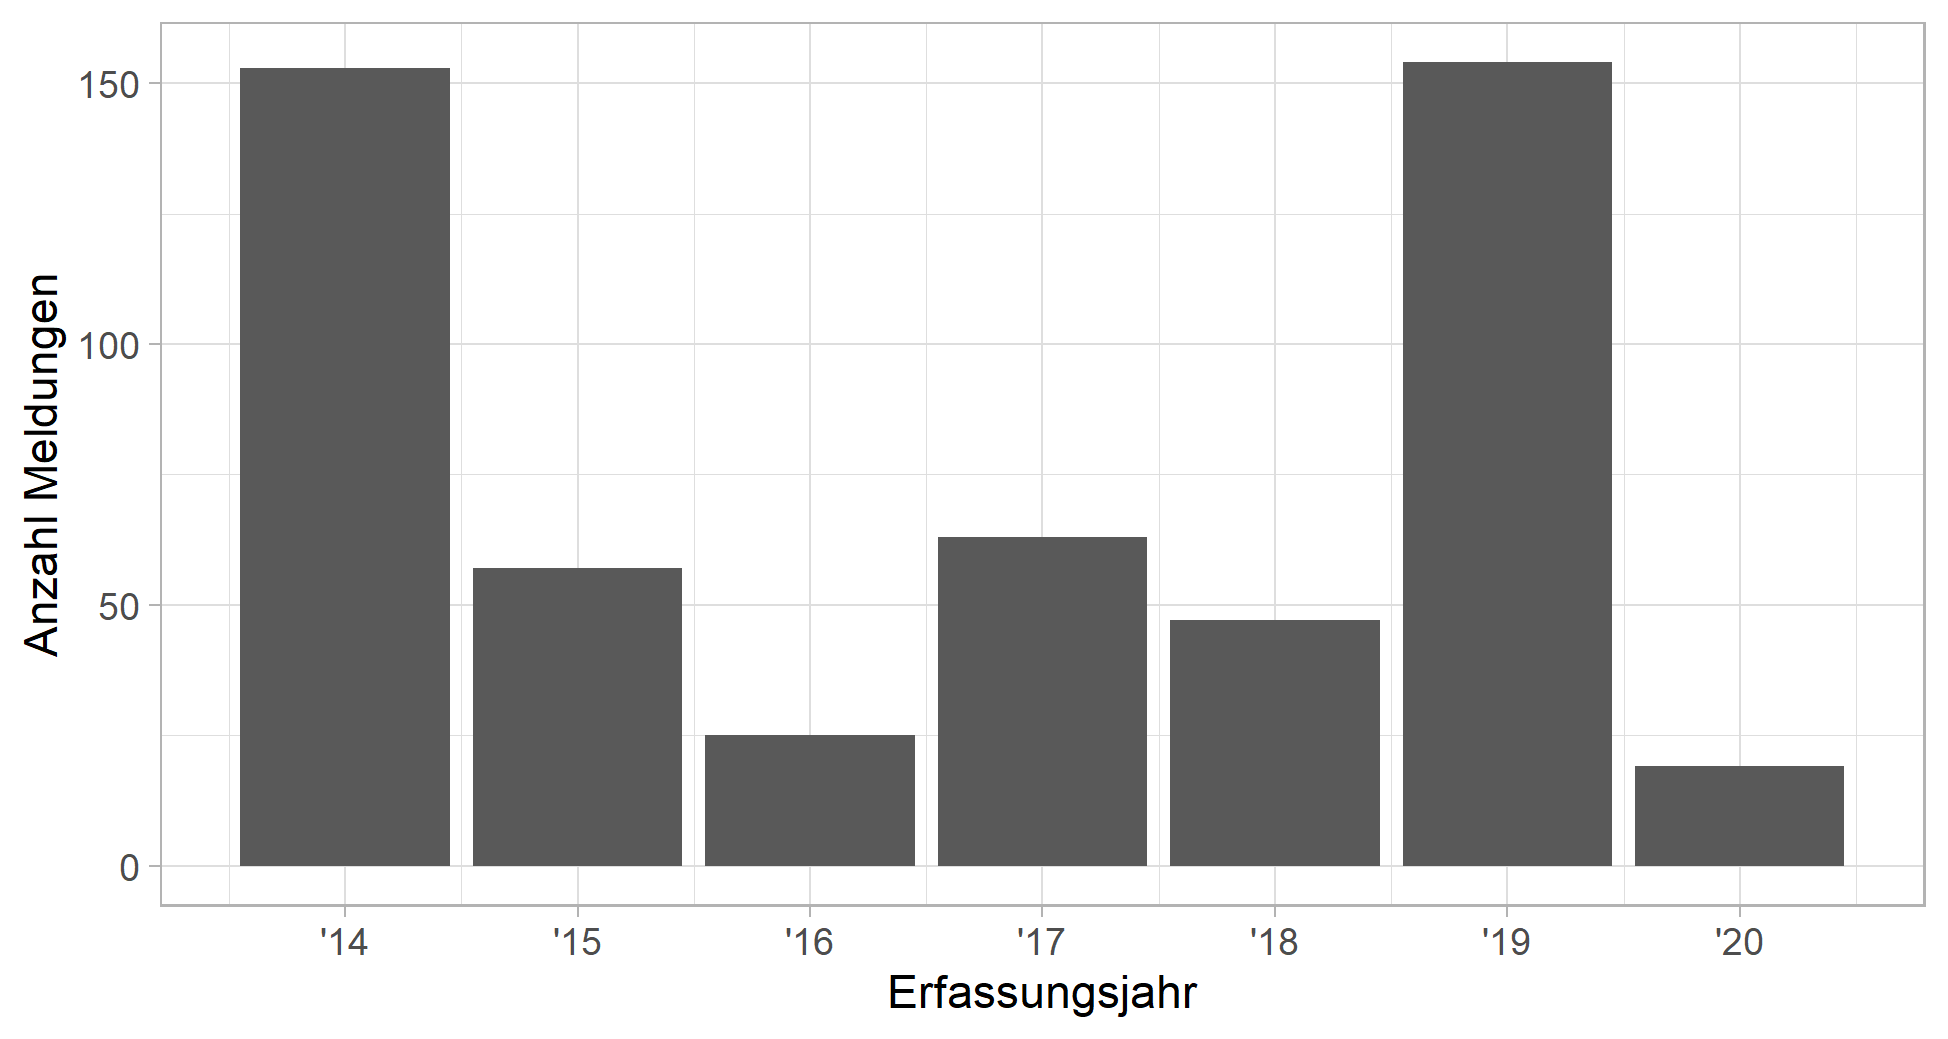
\includegraphics[width=1\linewidth]{images/beobachtungsmeldungen_histogramm} \caption{Anzahl gemeldete Beobachtungen pro Jahr, in dem die Meldung in die Datenbank eingetragen wurden. Die hohen Spitzen sind dadurch begründet, dass mehrere, schriftlich vorliegende Meldungen vom Projektleiter in der Datenbank erfasst wurden.}\label{fig:beobachtungsmeldungenhistogramm}
\end{figure}

\hypertarget{resultate}{%
\chapter{Resultate}\label{resultate}}

\hypertarget{erhebung-1-attraktivituxe4tskontrolle-von-asthaufen-mittels-spurentunneln-1}{%
\section{Erhebung 1: Attraktivitätskontrolle von Asthaufen mittels Spurentunneln}\label{erhebung-1-attraktivituxe4tskontrolle-von-asthaufen-mittels-spurentunneln-1}}

Anhand der Spurenpapiere konnten im Herbst 2019 32 Einzelnachweise von Hermelinen, sowie 2 Einzelnachweise von Iltissen aufgezeichnet werden. Die dritte Zielart, das Mauswiesel, konnte an keinem Standort nachgewiesen werden. Im Frühling 2020 konnten 23 Einzelnachweise von Hermelinen gemacht werden, jedoch keine vom Iltis oder vom Mauswiesel. Über beide Studien konnten somit 55 Einzelnachweise vom Hermelin und zwei Einzelnachweise vom Iltis gemacht werden (siehe Abbildung \ref{fig:wirkungskontrollesystematischeinzelnachweisewaffle}).



\begin{figure}
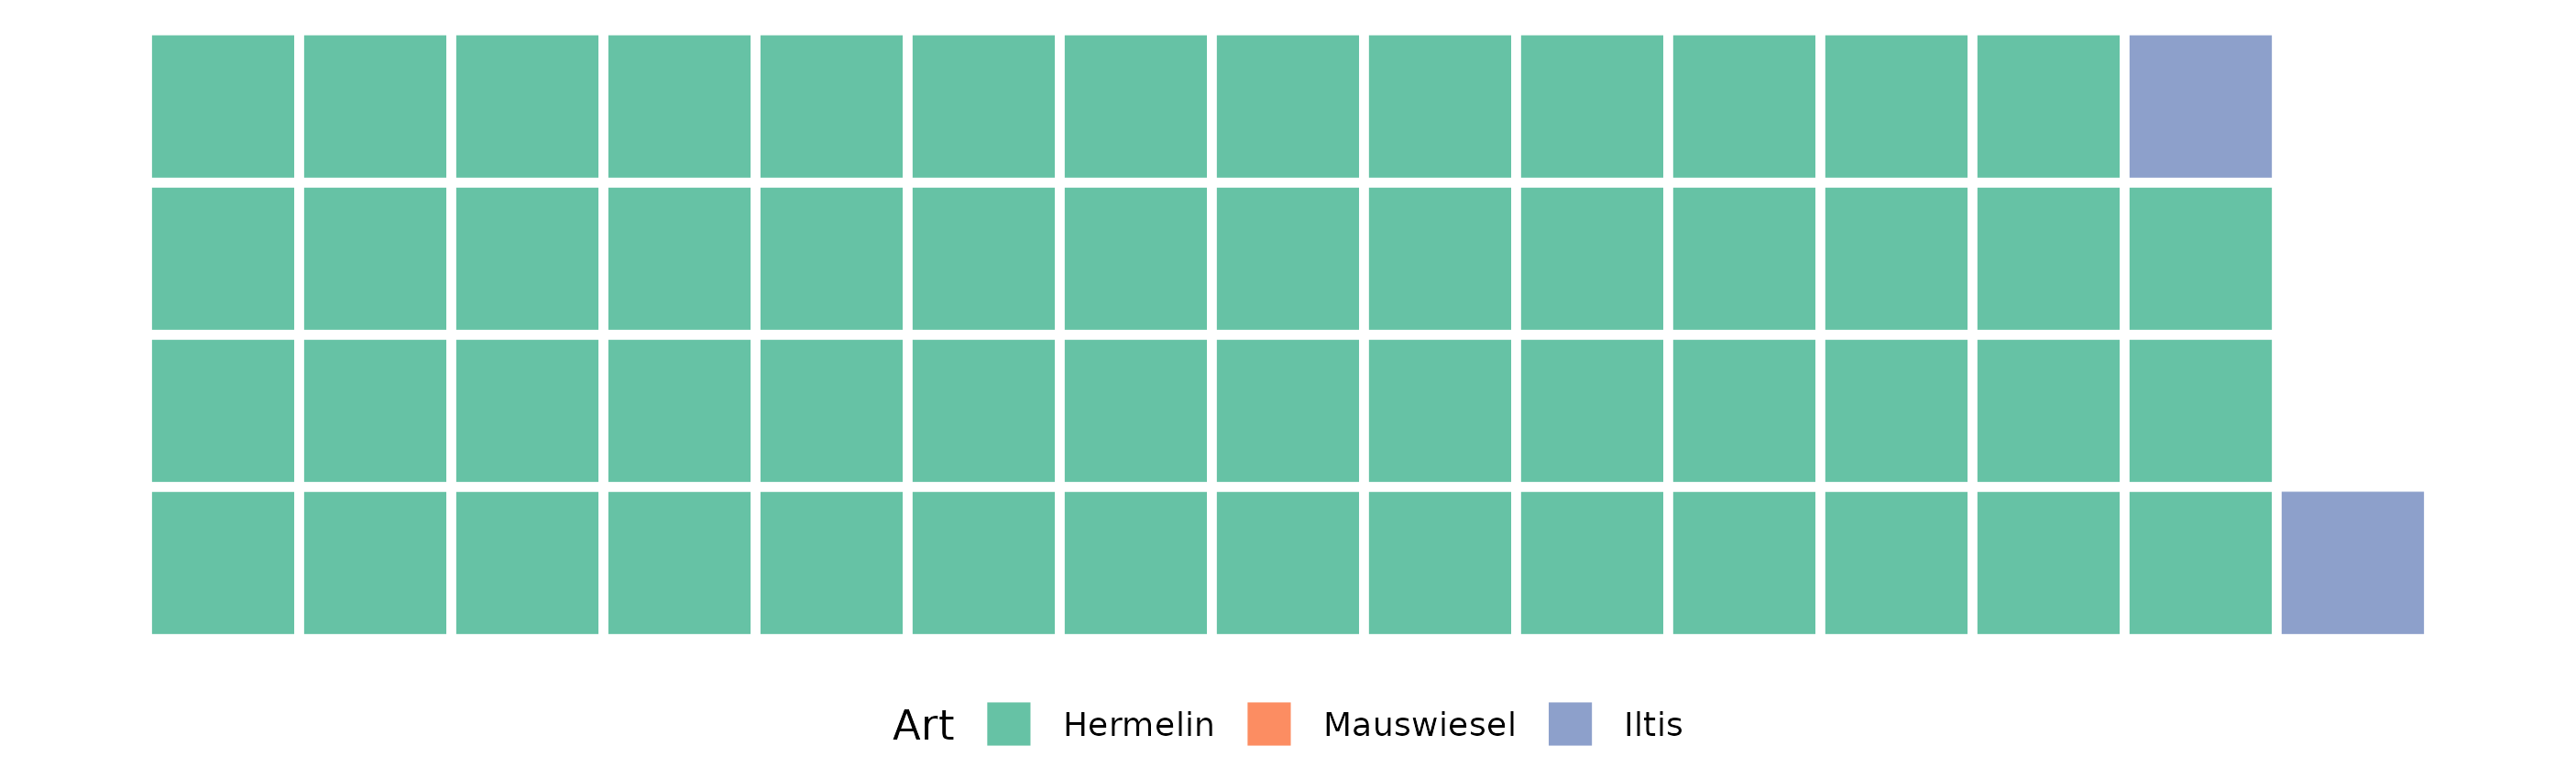
\includegraphics[width=1\linewidth]{images/wirkungskontrolle_systematisch_einzelnachweise_waffle} \caption{Anzahl Einzelnachweise pro Zielart über beide Untersuchungsperioden (Herbst 2019 und Frühling 2020): Insgesamt wurde das Hermelin 55-mal, der Iltis 2-mal und das Mauswiesel gar nicht nachgewiesen.}\label{fig:wirkungskontrollesystematischeinzelnachweisewaffle}
\end{figure}

Da es sich bei gewissen Nachweisen vermutlich um Mehrfachbeobachtung des gleichen Individuums handelt, ist der Anteil an Strukturen mit mindestens einem Nachweis aussagekräftiger. Im Herbst 2019 konnte in 19 von 39 Asthaufen (49 \%) mindestens eine Zielart nachgewiesen werden. In 18 von 39 Asthaufen (46 \%) wurde das Hermelin detektiert, in 2 von 39 Asthaufen (5 \%) der Iltis. Im Frühling 2020 wurde in 14 von 39 Asthaufen (36 \%) eine Zielart detektiert, wobei es sich immer um Hermeline handelte (siehe Abbildung \ref{fig:strukturenmitzielart}). Über beide Untersuchungsperioden hinweg konnte in 27 von 39 Asthaufen (69 \%) mindestens eine Zielart detektiert werden.



\begin{figure}
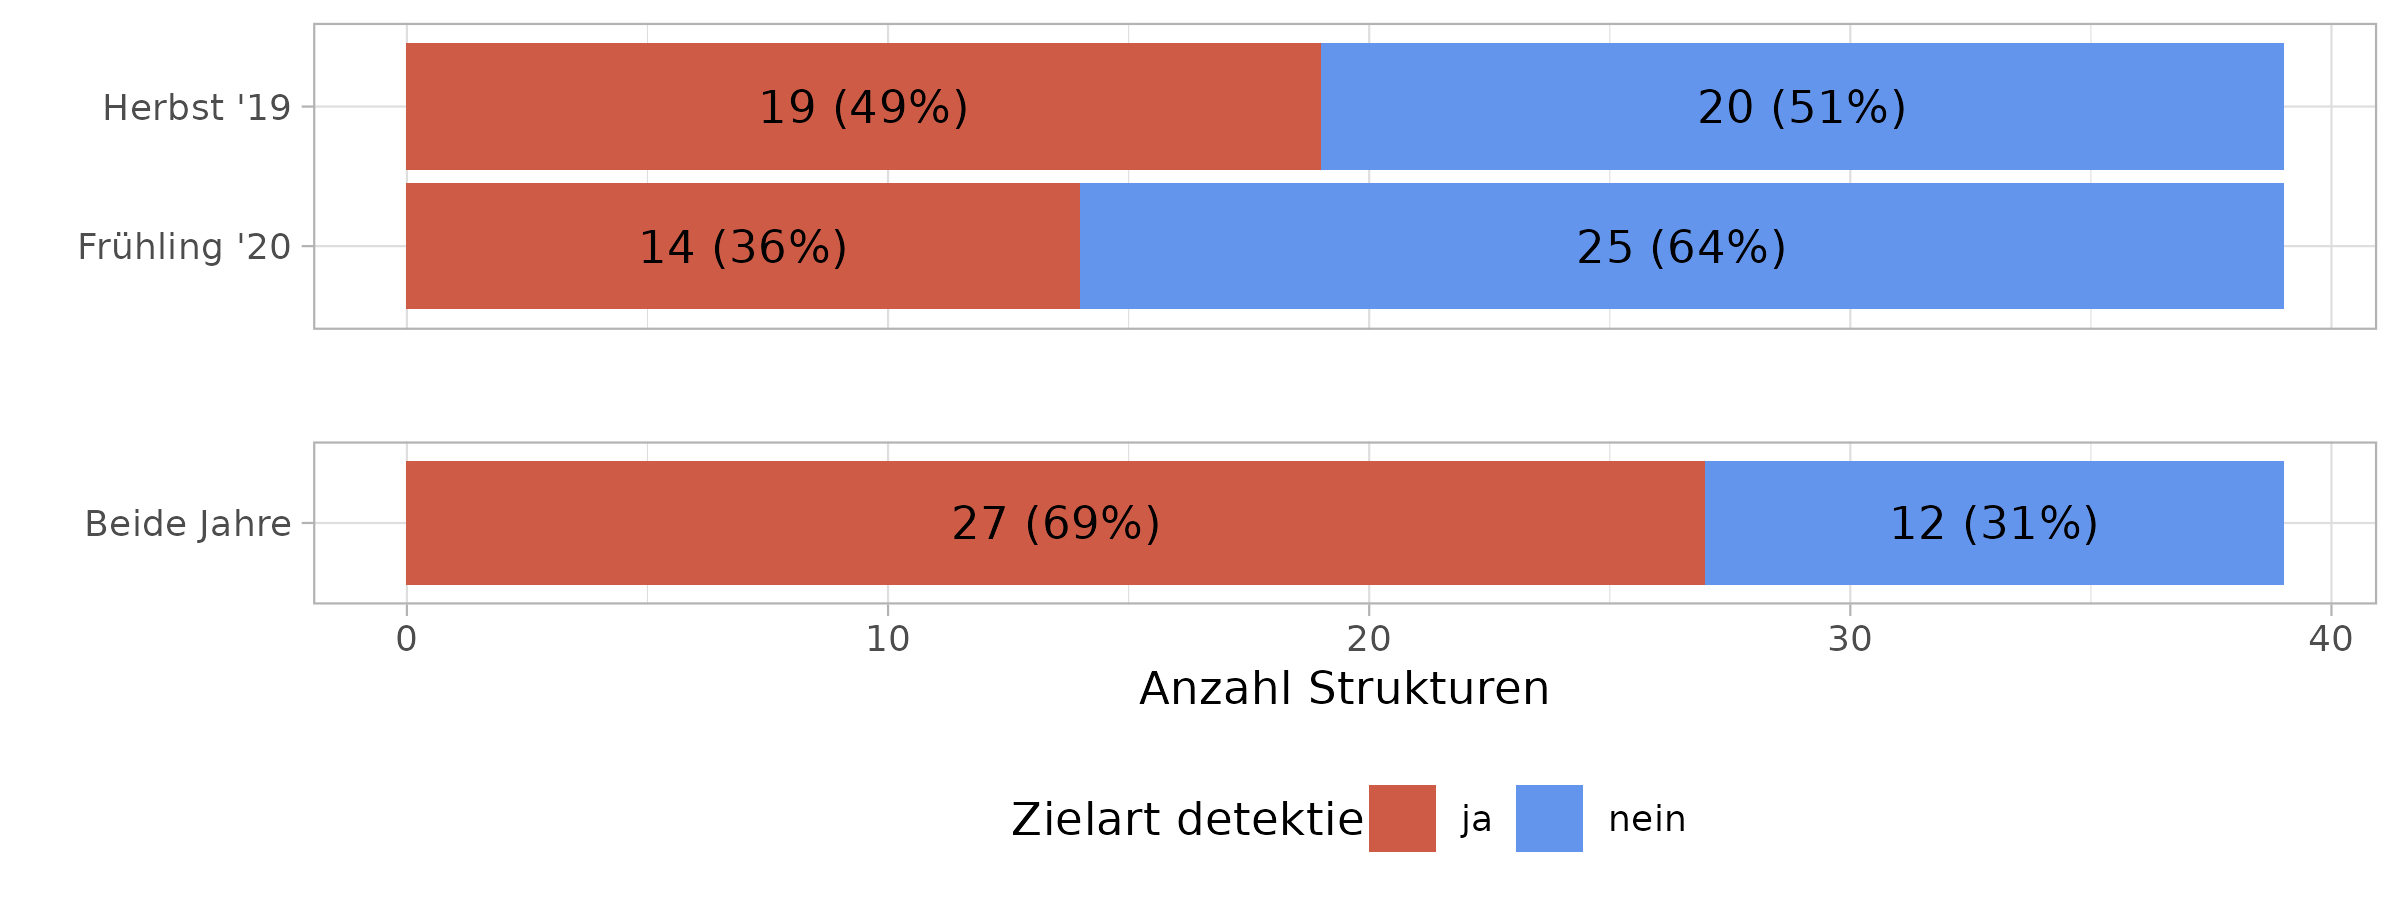
\includegraphics[width=1\linewidth]{images/strukturen_mit_zielart} \caption{Anzahl sowie Anteil der untersuchten Strukturen, in denen mindestens eine Zielart nachgewiesen werden konnte.}\label{fig:strukturenmitzielart}
\end{figure}



\begin{figure}
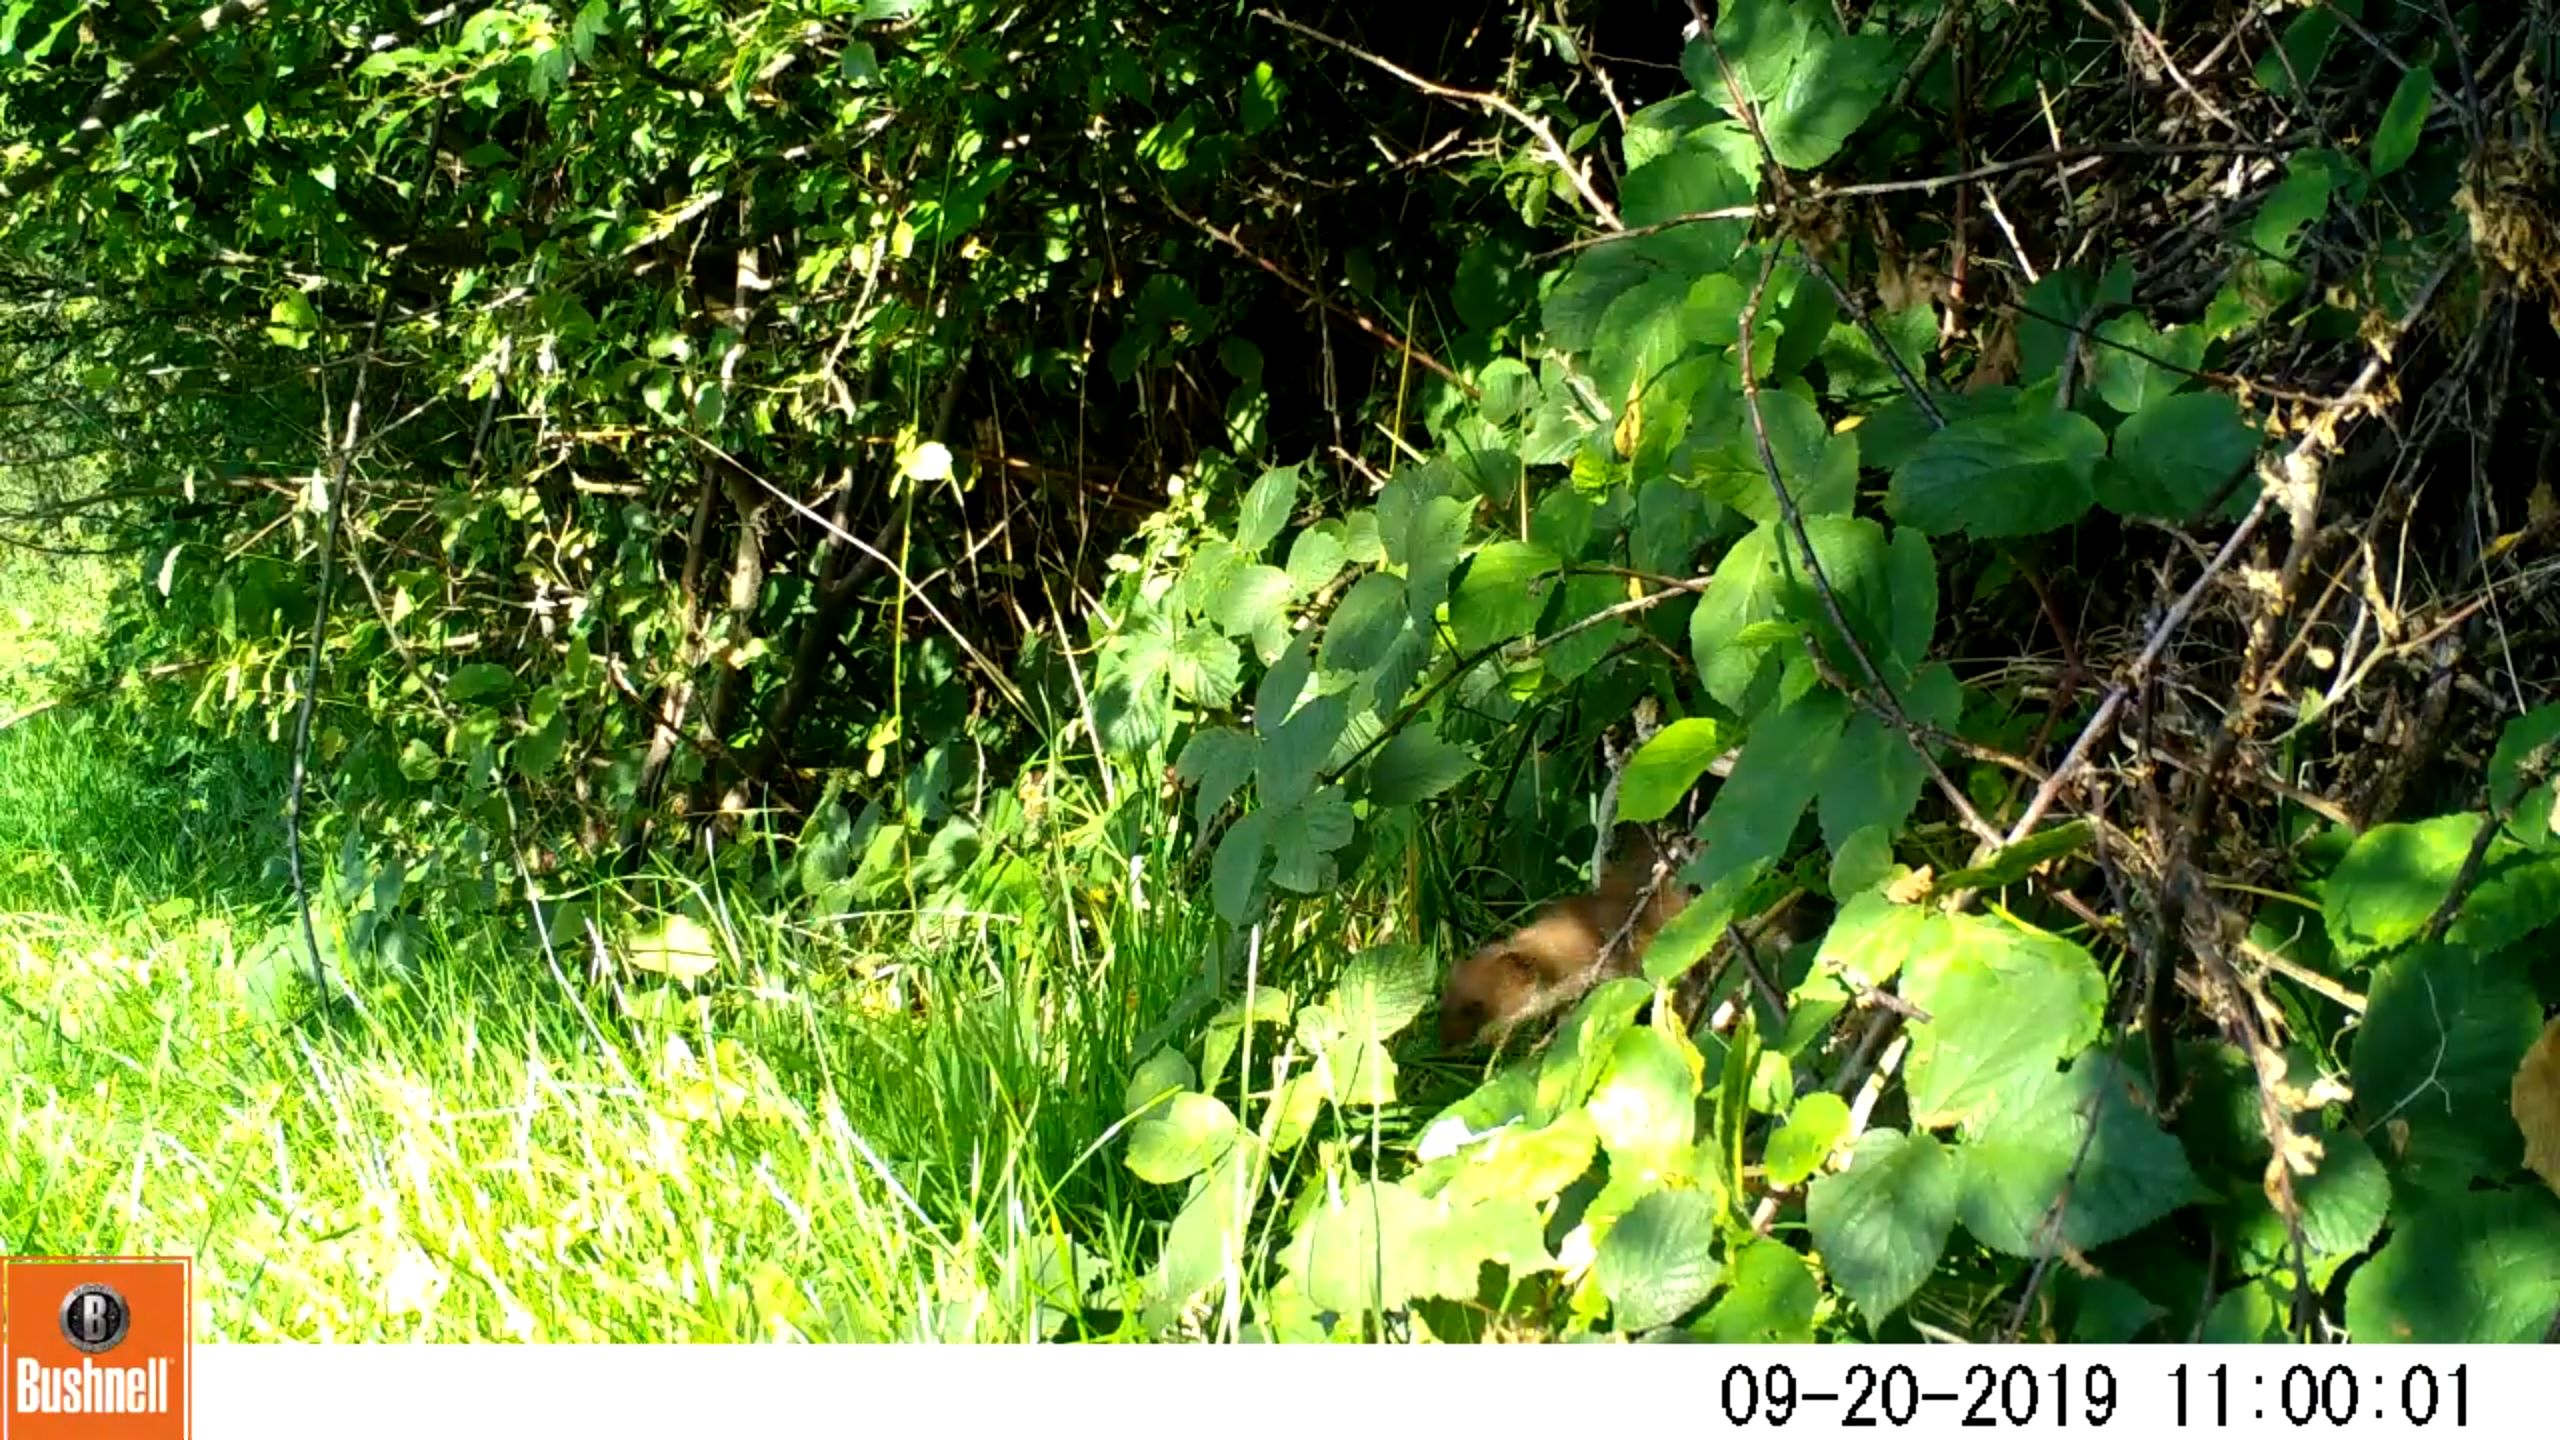
\includegraphics[width=1\linewidth]{images/str196/capture} \caption{Ein Hermelin, welches einen im Projekt erstellten Asthaufen als Deckungsstruktur nutzt.}\label{fig:hermelinstr196}
\end{figure}

\begin{figure}[hbt!] \centering 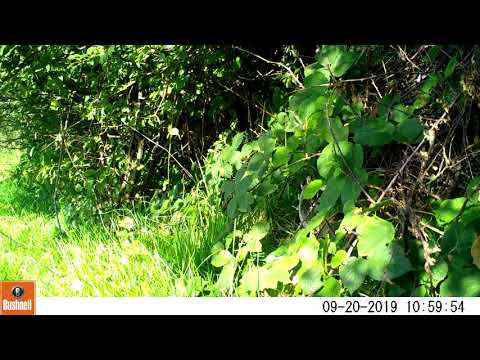
\includegraphics{images/youtube/4gVpcvPIrNA.jpg} \caption{Der Video ist in voller Länge hier abgespeichert: \url{https://youtu.be/4gVpcvPIrNA}} \end{figure}

\hypertarget{erhebung-2-attraktivituxe4tskontrolle-von-winterquartieren-mittels-fotofallen-1}{%
\section{Erhebung 2: Attraktivitätskontrolle von Winterquartieren mittels Fotofallen}\label{erhebung-2-attraktivituxe4tskontrolle-von-winterquartieren-mittels-fotofallen-1}}

Aus der Fotofallen-Überwachung der Winterquartiere resultierten 2019 an zwei Standorten Aufnahmen von Hermelinen, sowie an zwei Standorten von Iltissen (siehe Abbildung \ref{fig:winterquartiereresultate}). Im Folgejahr (2020) gelangen Nachweise vom Hermelin an einem neuen Standort und vom Iltis an einem Standort mit Nachweis im Frühling 2019. Zusammenfassend über beide Jahre kann gesagt werden, dass in 5 von 11 untersuchten Winterquartieren (45\%) mindestens eine Zielart festgestellt werden konnte (4 Hermelin- und 3 Iltis-Nachweise). Alle 3 Winterquartiere in Feldscheunen (sanierte Streuhütten) wiesen Nachweise auf (2 des Hermelins, 3 des Iltis).
Jedes Winterquartier wurde von zahlreichen Tierarten genutzt: Dachse, Eichhörnchen, Füchse, Marder, Frösche, Vögel und Mäusen wurden von den Kameras abgelichtet.

Die Daten der Standorte Str116 und Str198 konnten 2019 und die von Str12747 im Jahr 2020 nicht ausgewertet werden. Die Kameras an den genannten Standorten wiesen eine Fehlfunktion auf und erfassten so viele Bilder, dass eine Auswertung der Daten unverhältnismässig viel Zeit in Anspruch genommen hätte.



\begin{figure}
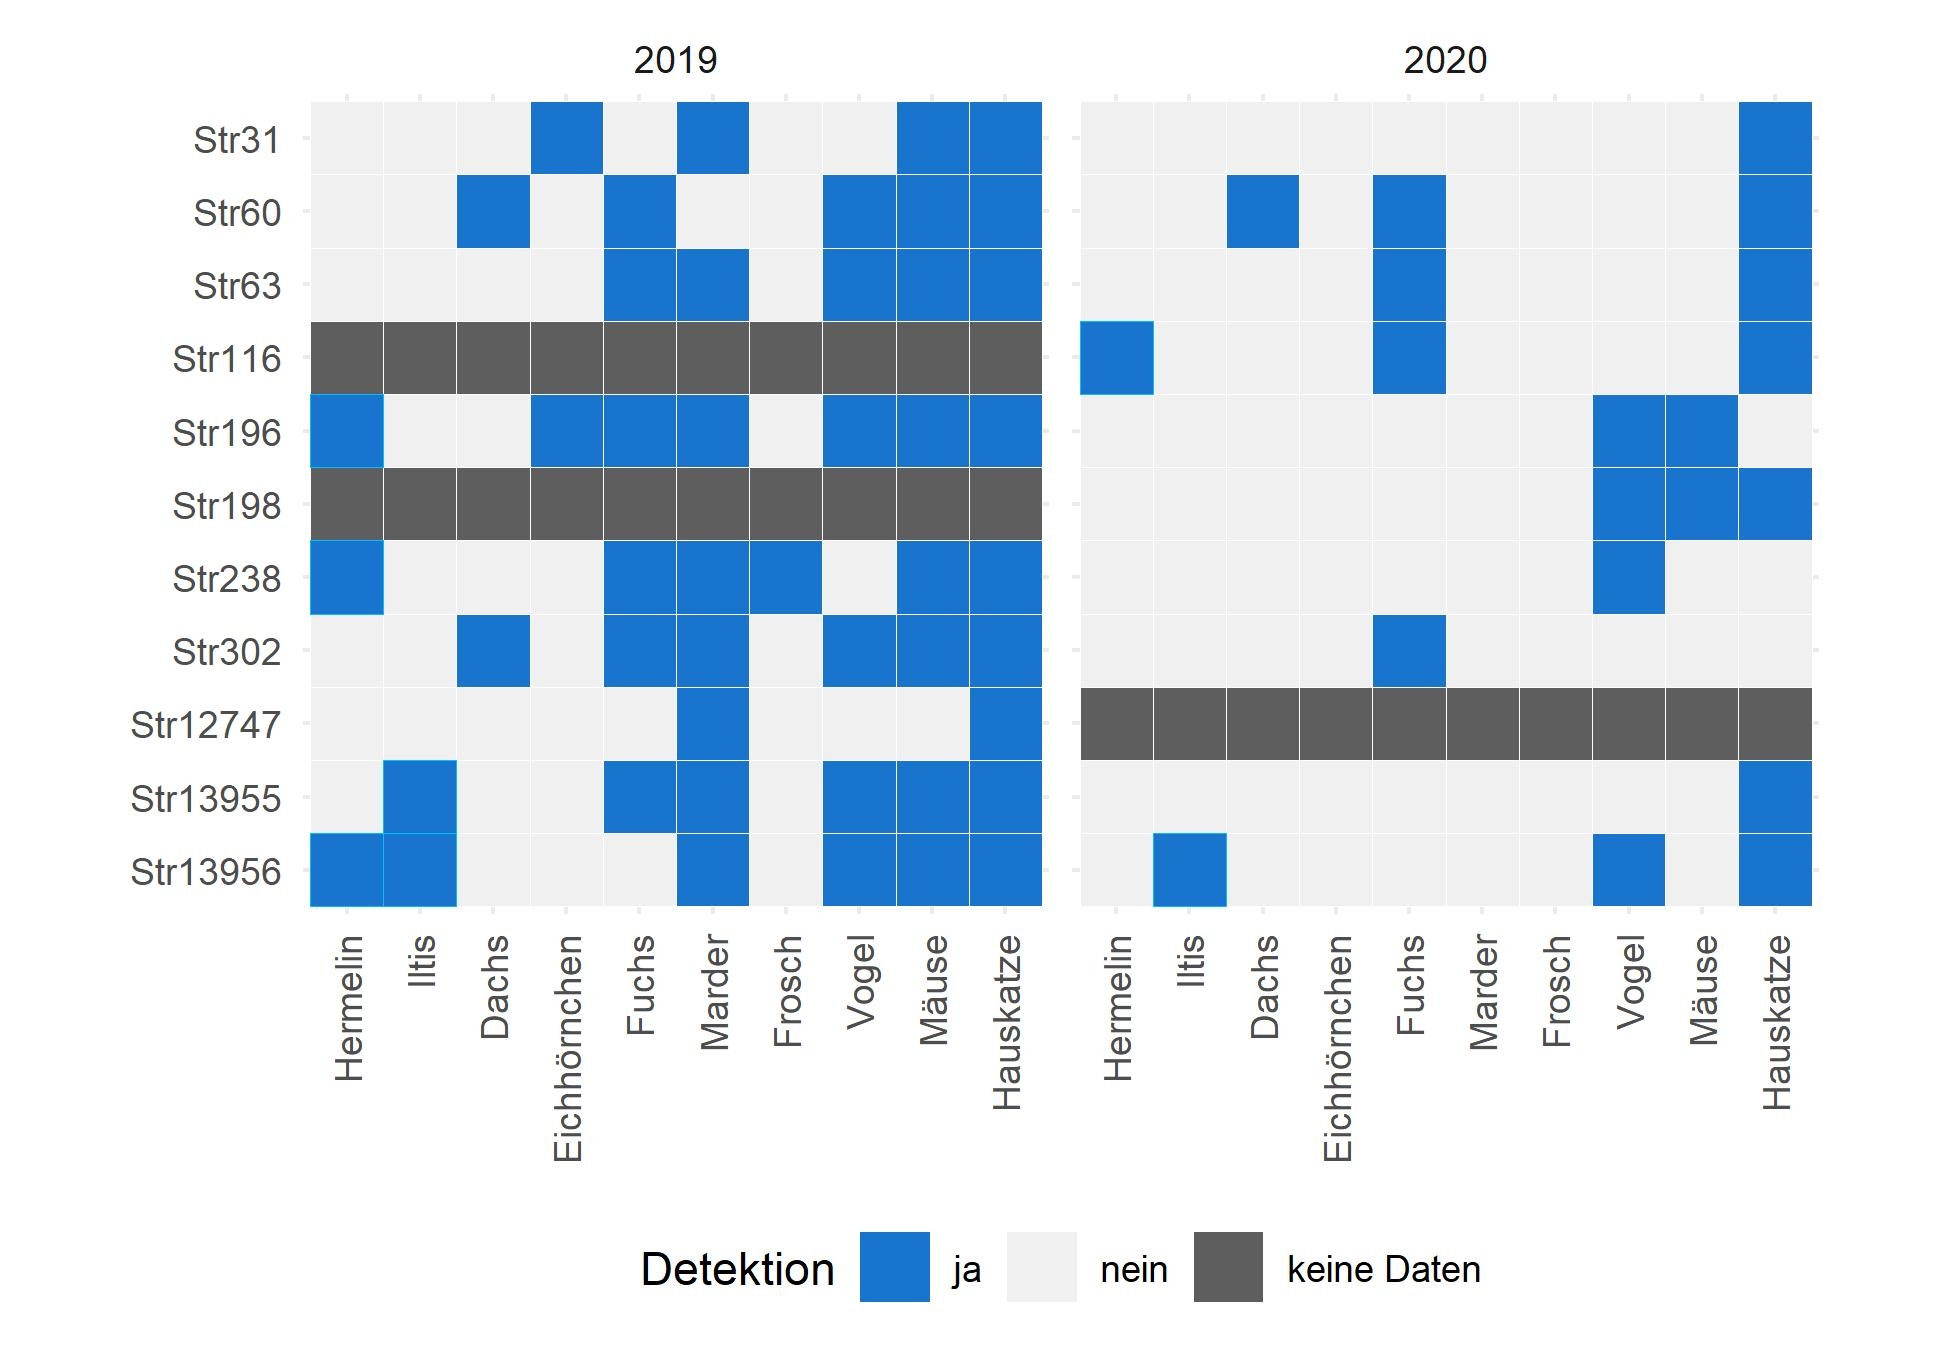
\includegraphics[width=1\linewidth]{images/winterquartiere_resultate} \caption{Zusammenfassung der Resultate aus der Überwachung der Winterquartiere mit sämtlichen Tierarten}\label{fig:winterquartiereresultate}
\end{figure}

\begin{figure}
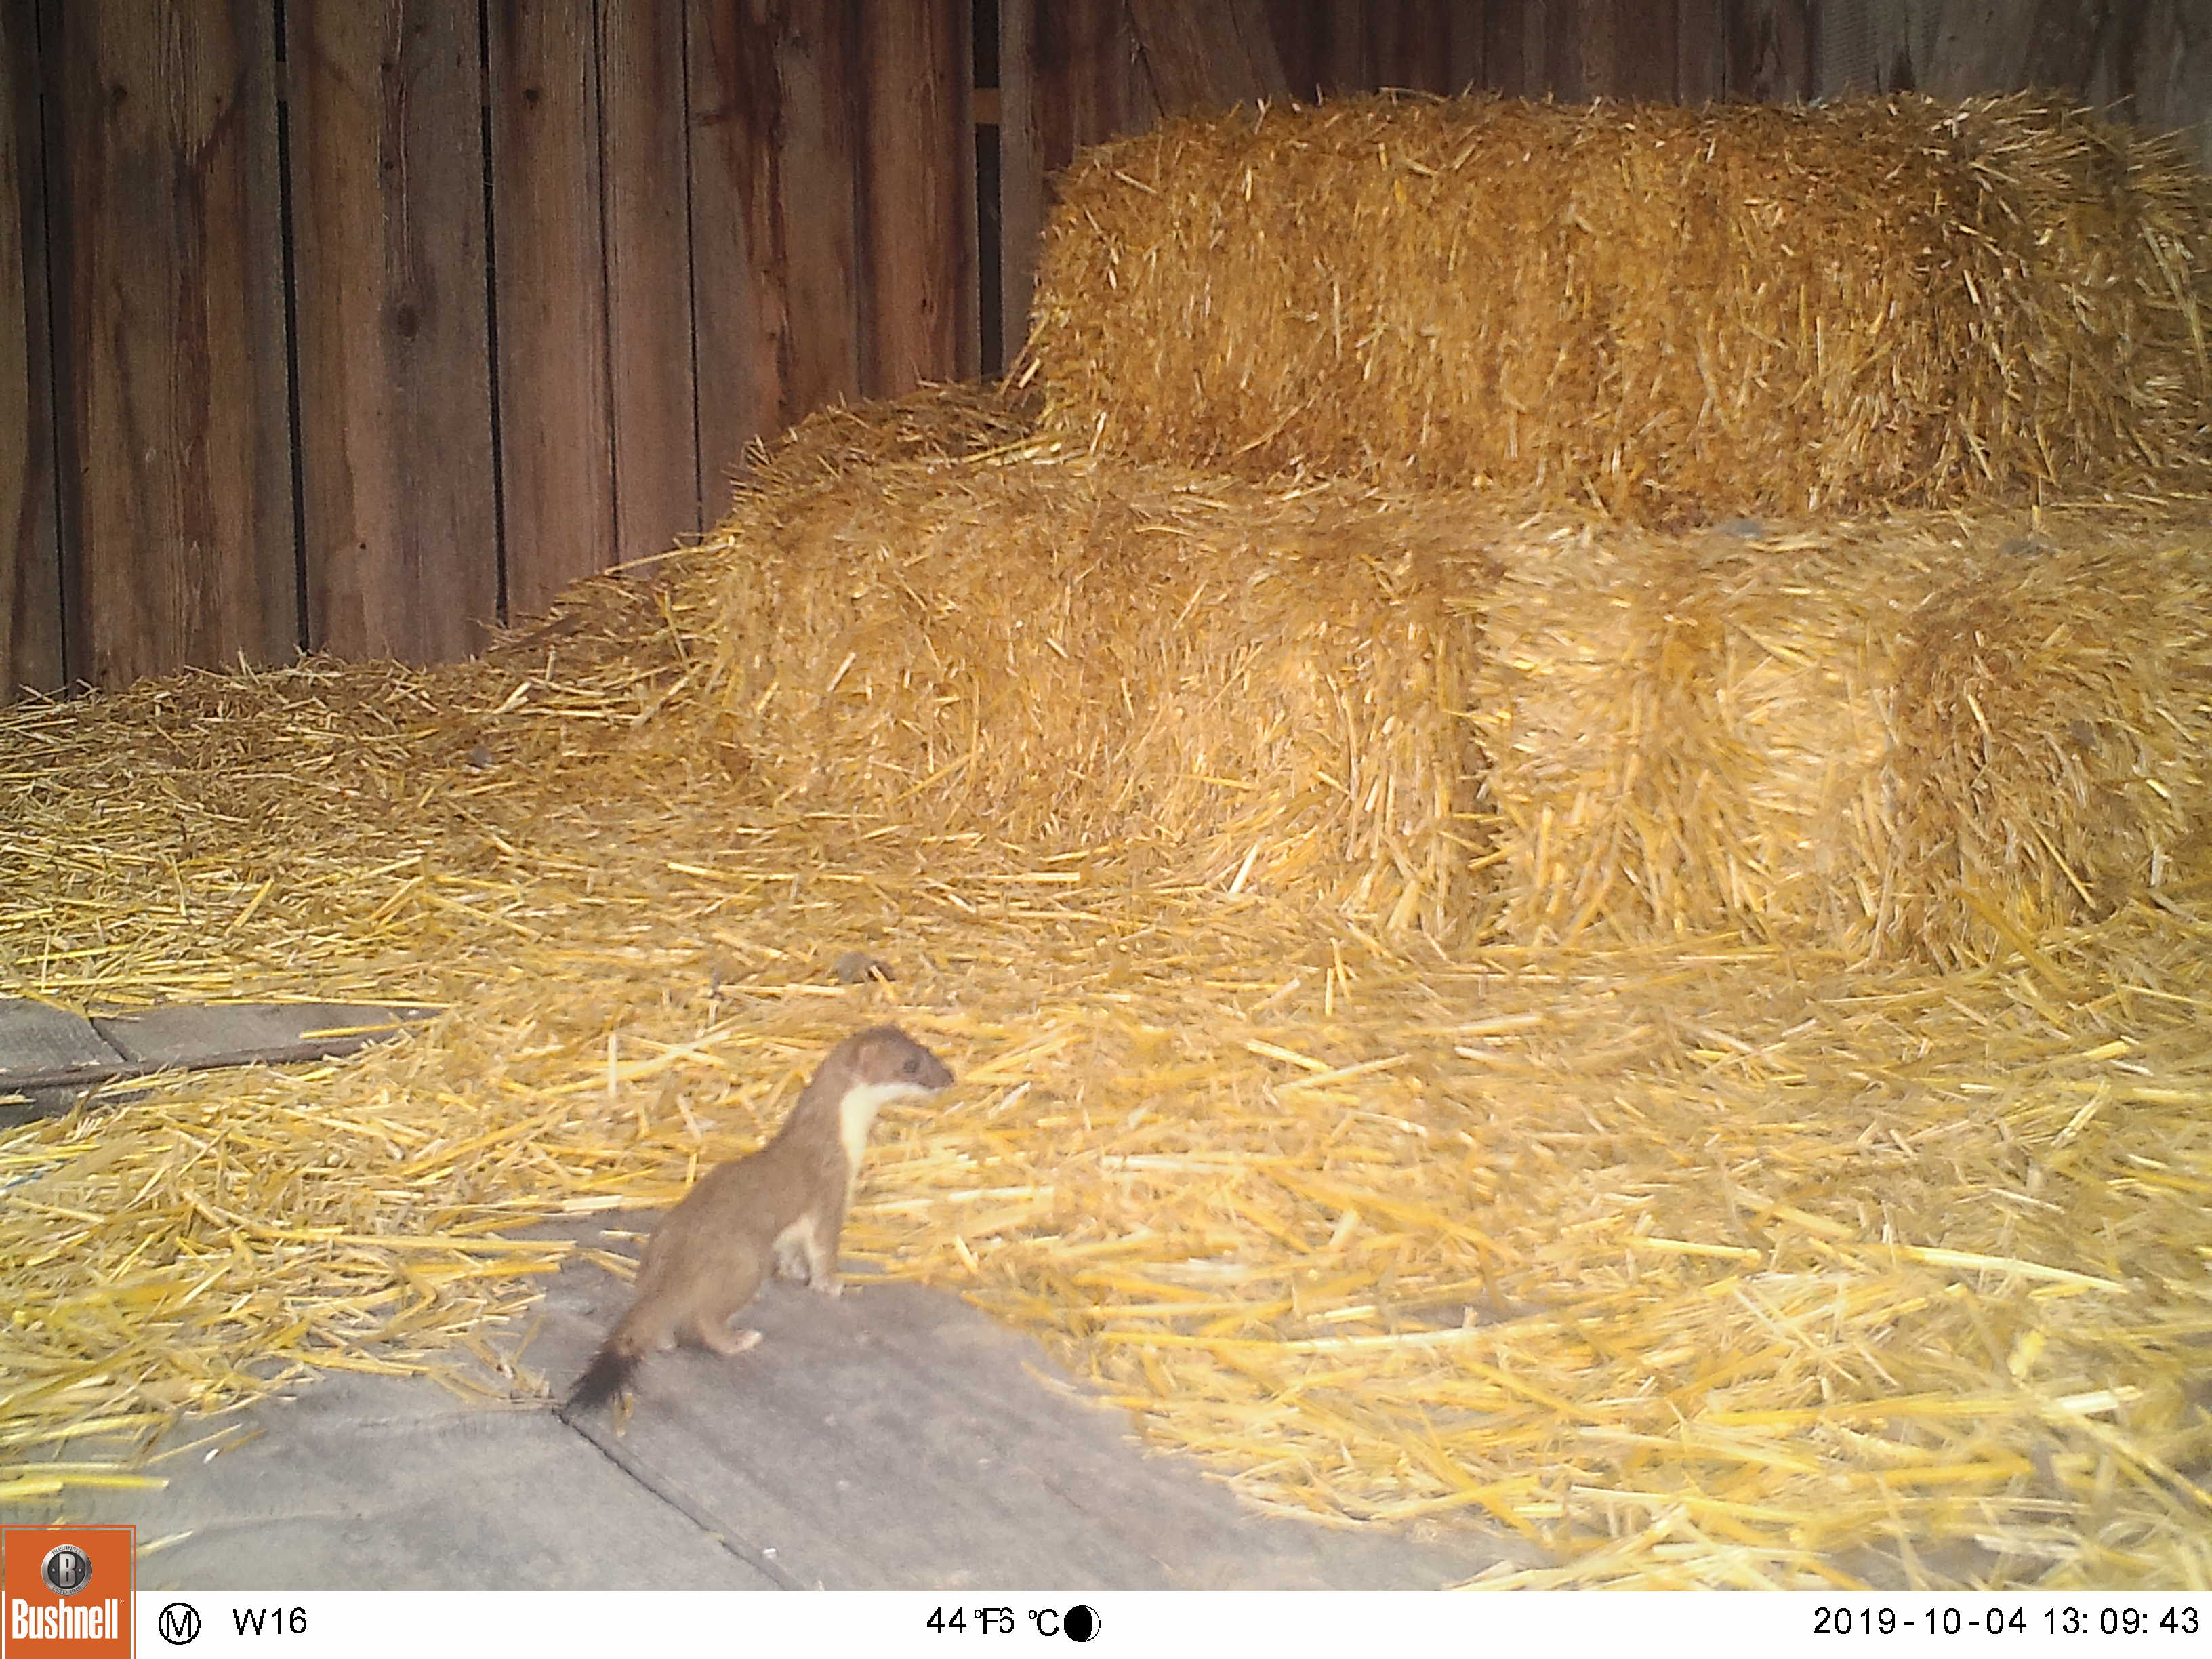
\includegraphics[width=0.49\linewidth]{images/str238//10040255} 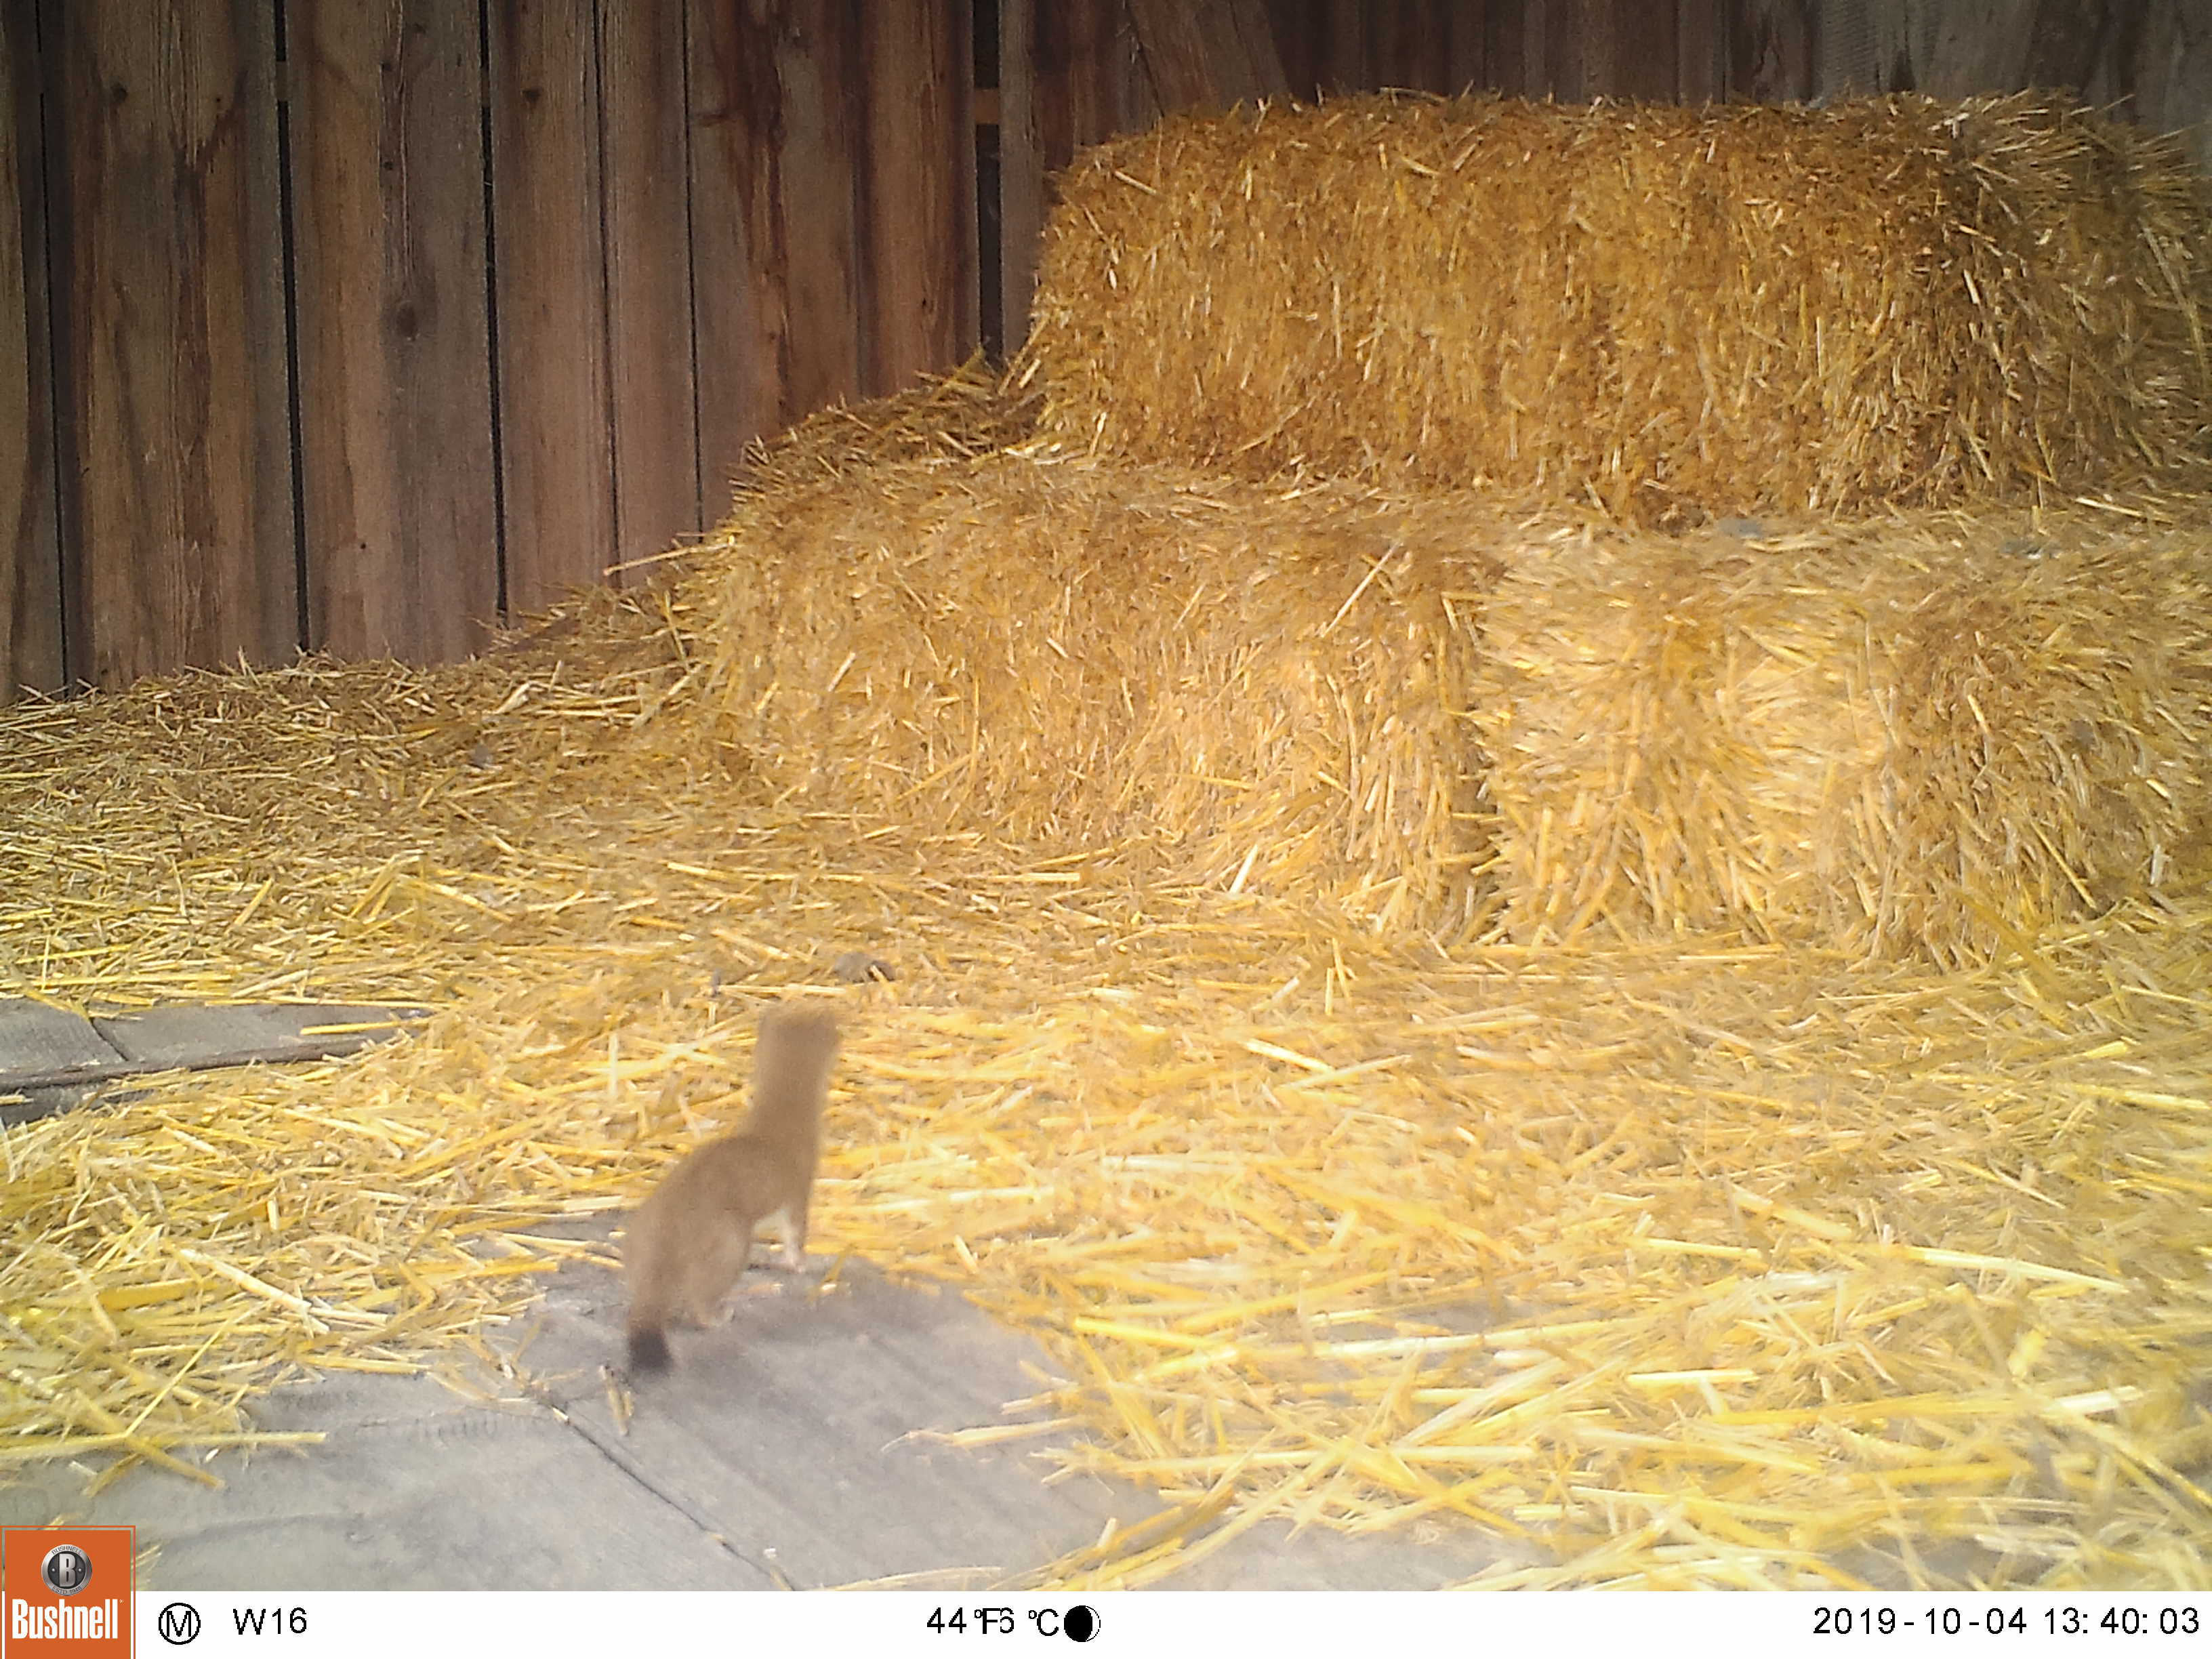
\includegraphics[width=0.49\linewidth]{images/str238//10040261} 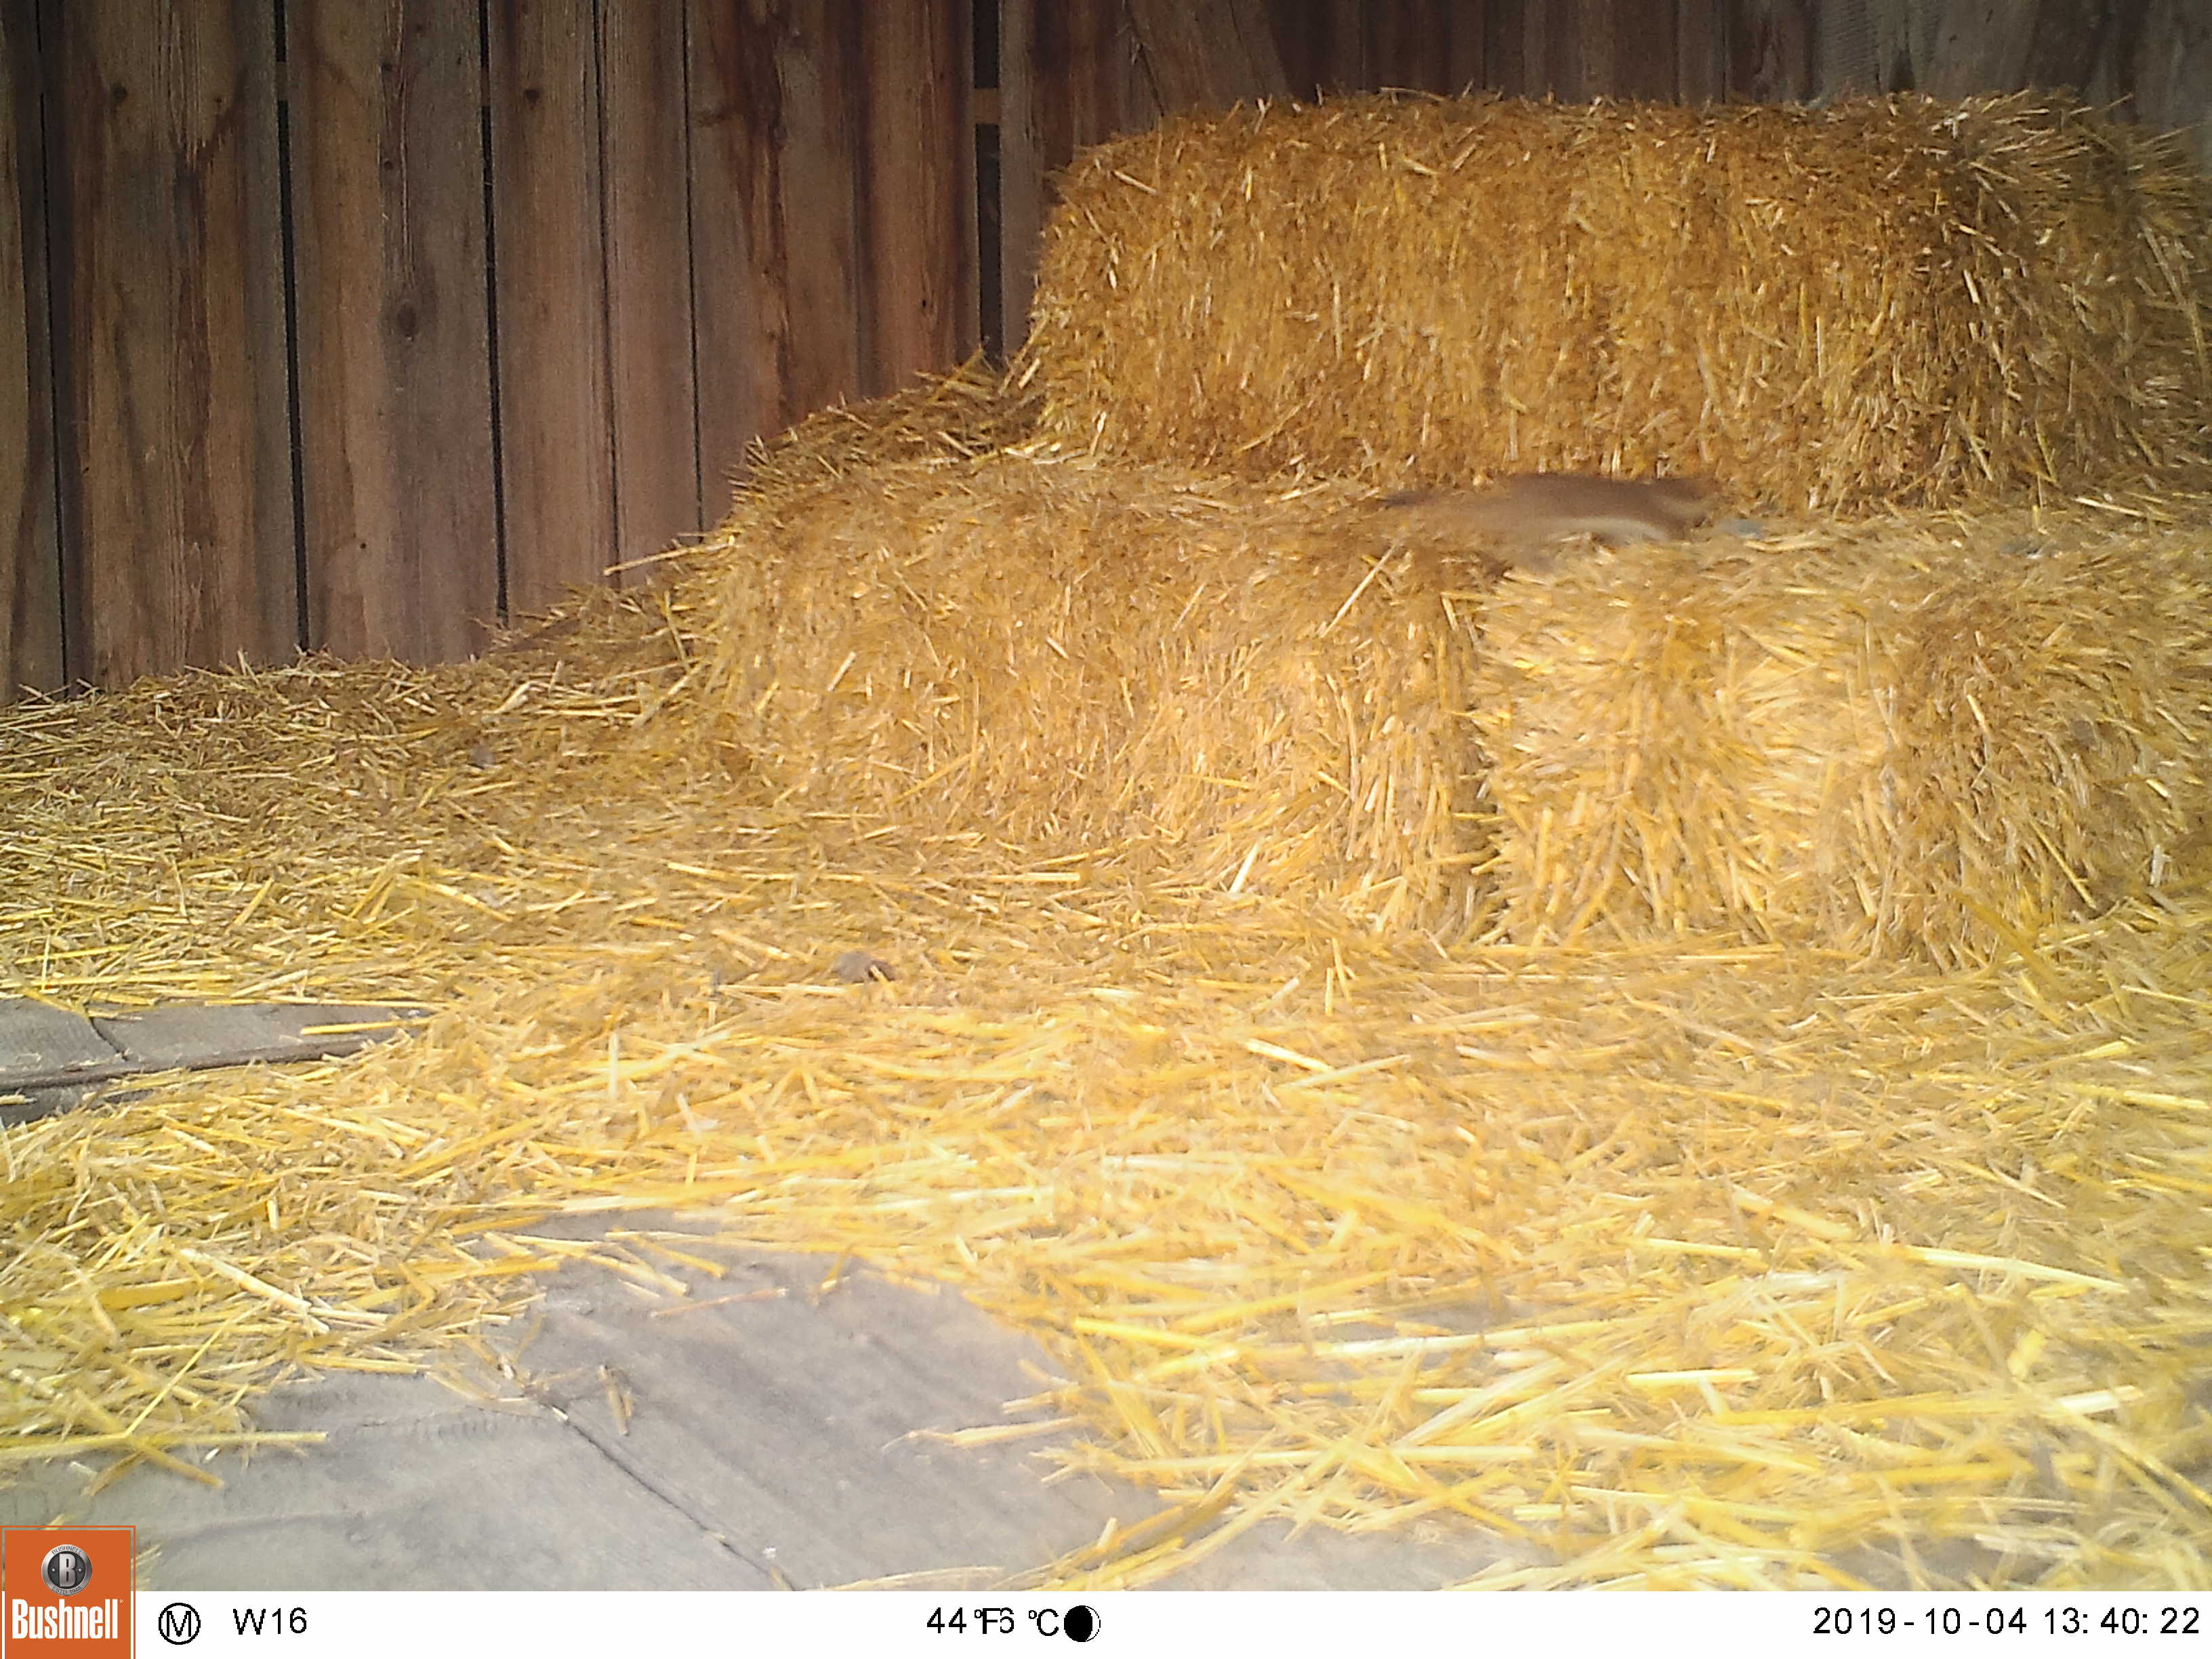
\includegraphics[width=0.49\linewidth]{images/str238//10040263} 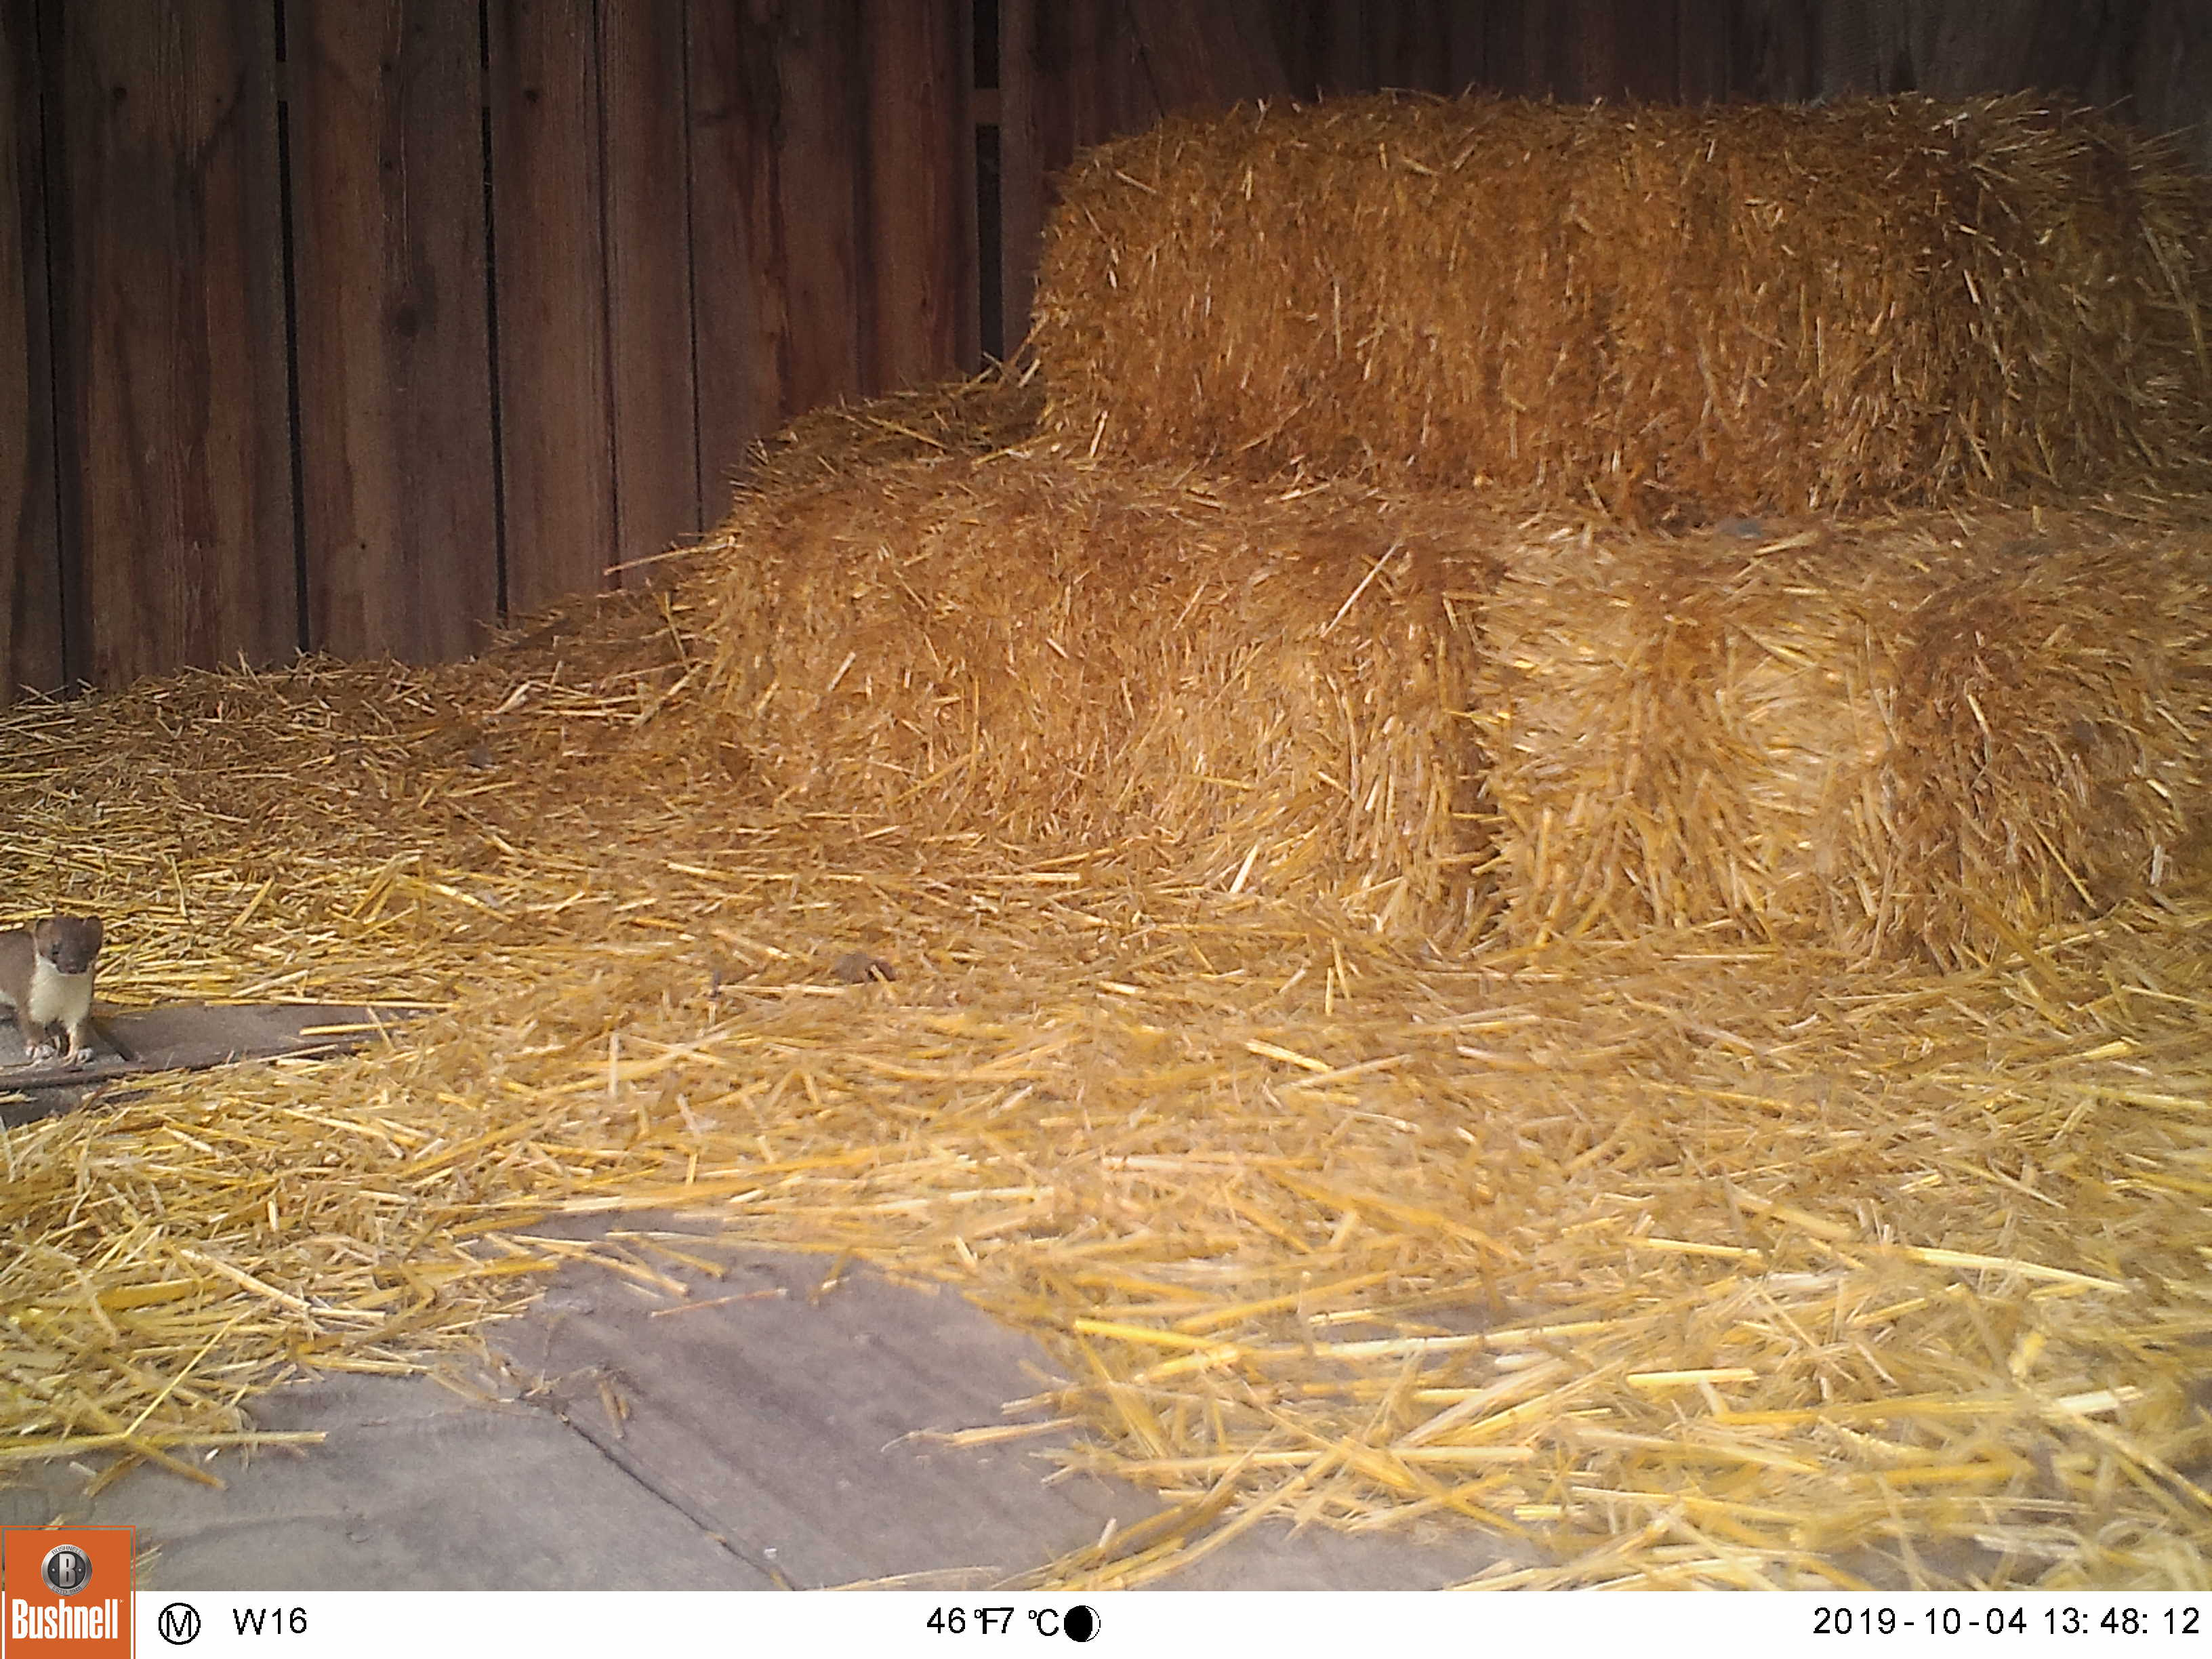
\includegraphics[width=0.49\linewidth]{images/str238//10040267} \caption{Bilderserien zeugen davon, dass die Winterquartiere von den Zielarten genutzt werden. Das Hermelin im Bild nutzt das kleine Schlupfloch und erkundet den geschützten Hohlraum, der durch die Anordnung der Strohballen besteht (Str. 238)}\label{fig:unnamed-chunk-5}
\end{figure}

\begin{figure}[hbt!] \centering 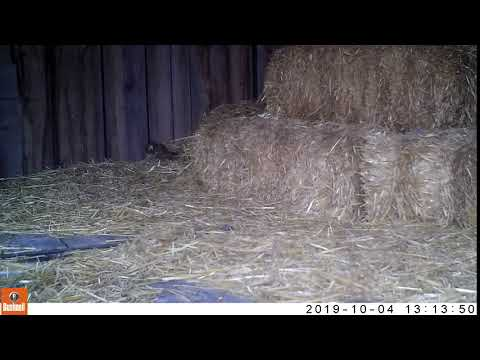
\includegraphics{images/youtube/YomCsy1olBs.jpg} \caption{Der Video ist in voller Länge hier abgespeichert: \url{https://youtu.be/YomCsy1olBs}} \end{figure}\begin{figure}[hbt!] \centering 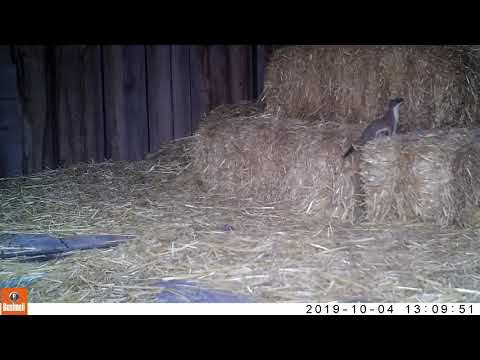
\includegraphics{images/youtube/ttv-LHkzc18.jpg} \caption{Der Video ist in voller Länge hier abgespeichert: \url{https://youtu.be/ttv-LHkzc18}} \end{figure}

\begin{figure}
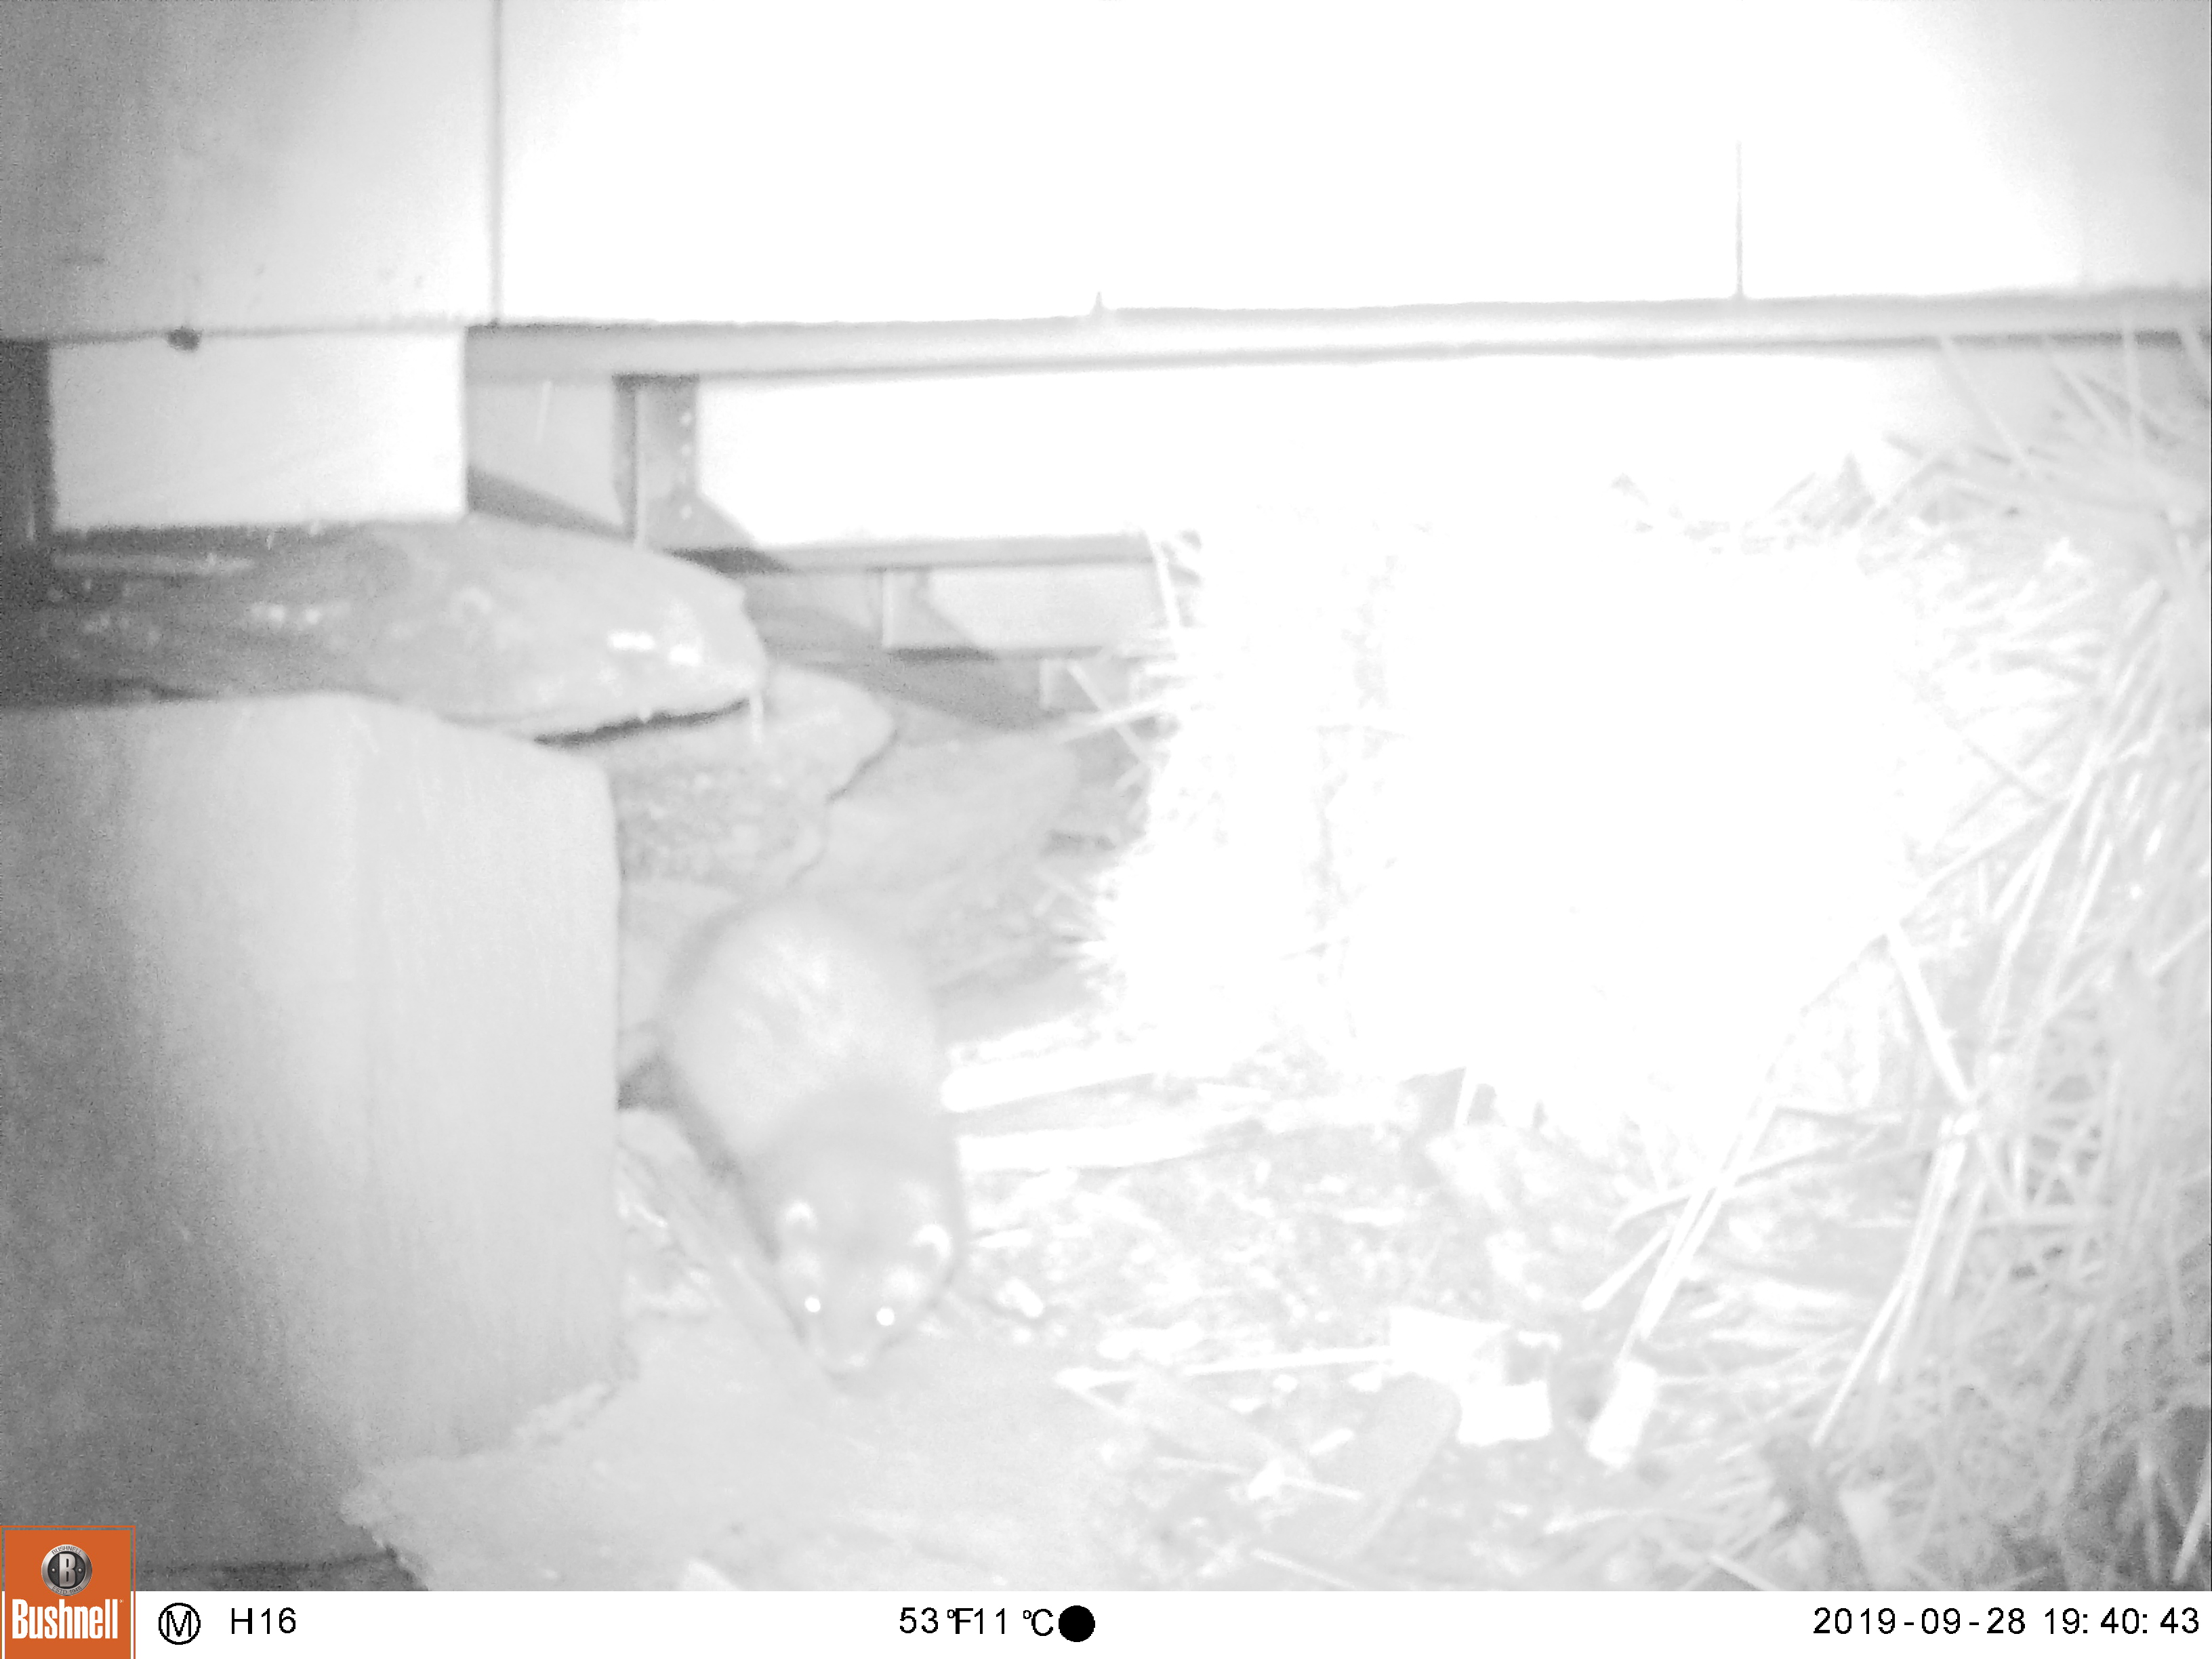
\includegraphics[width=1\linewidth]{images/str13956/09280317} 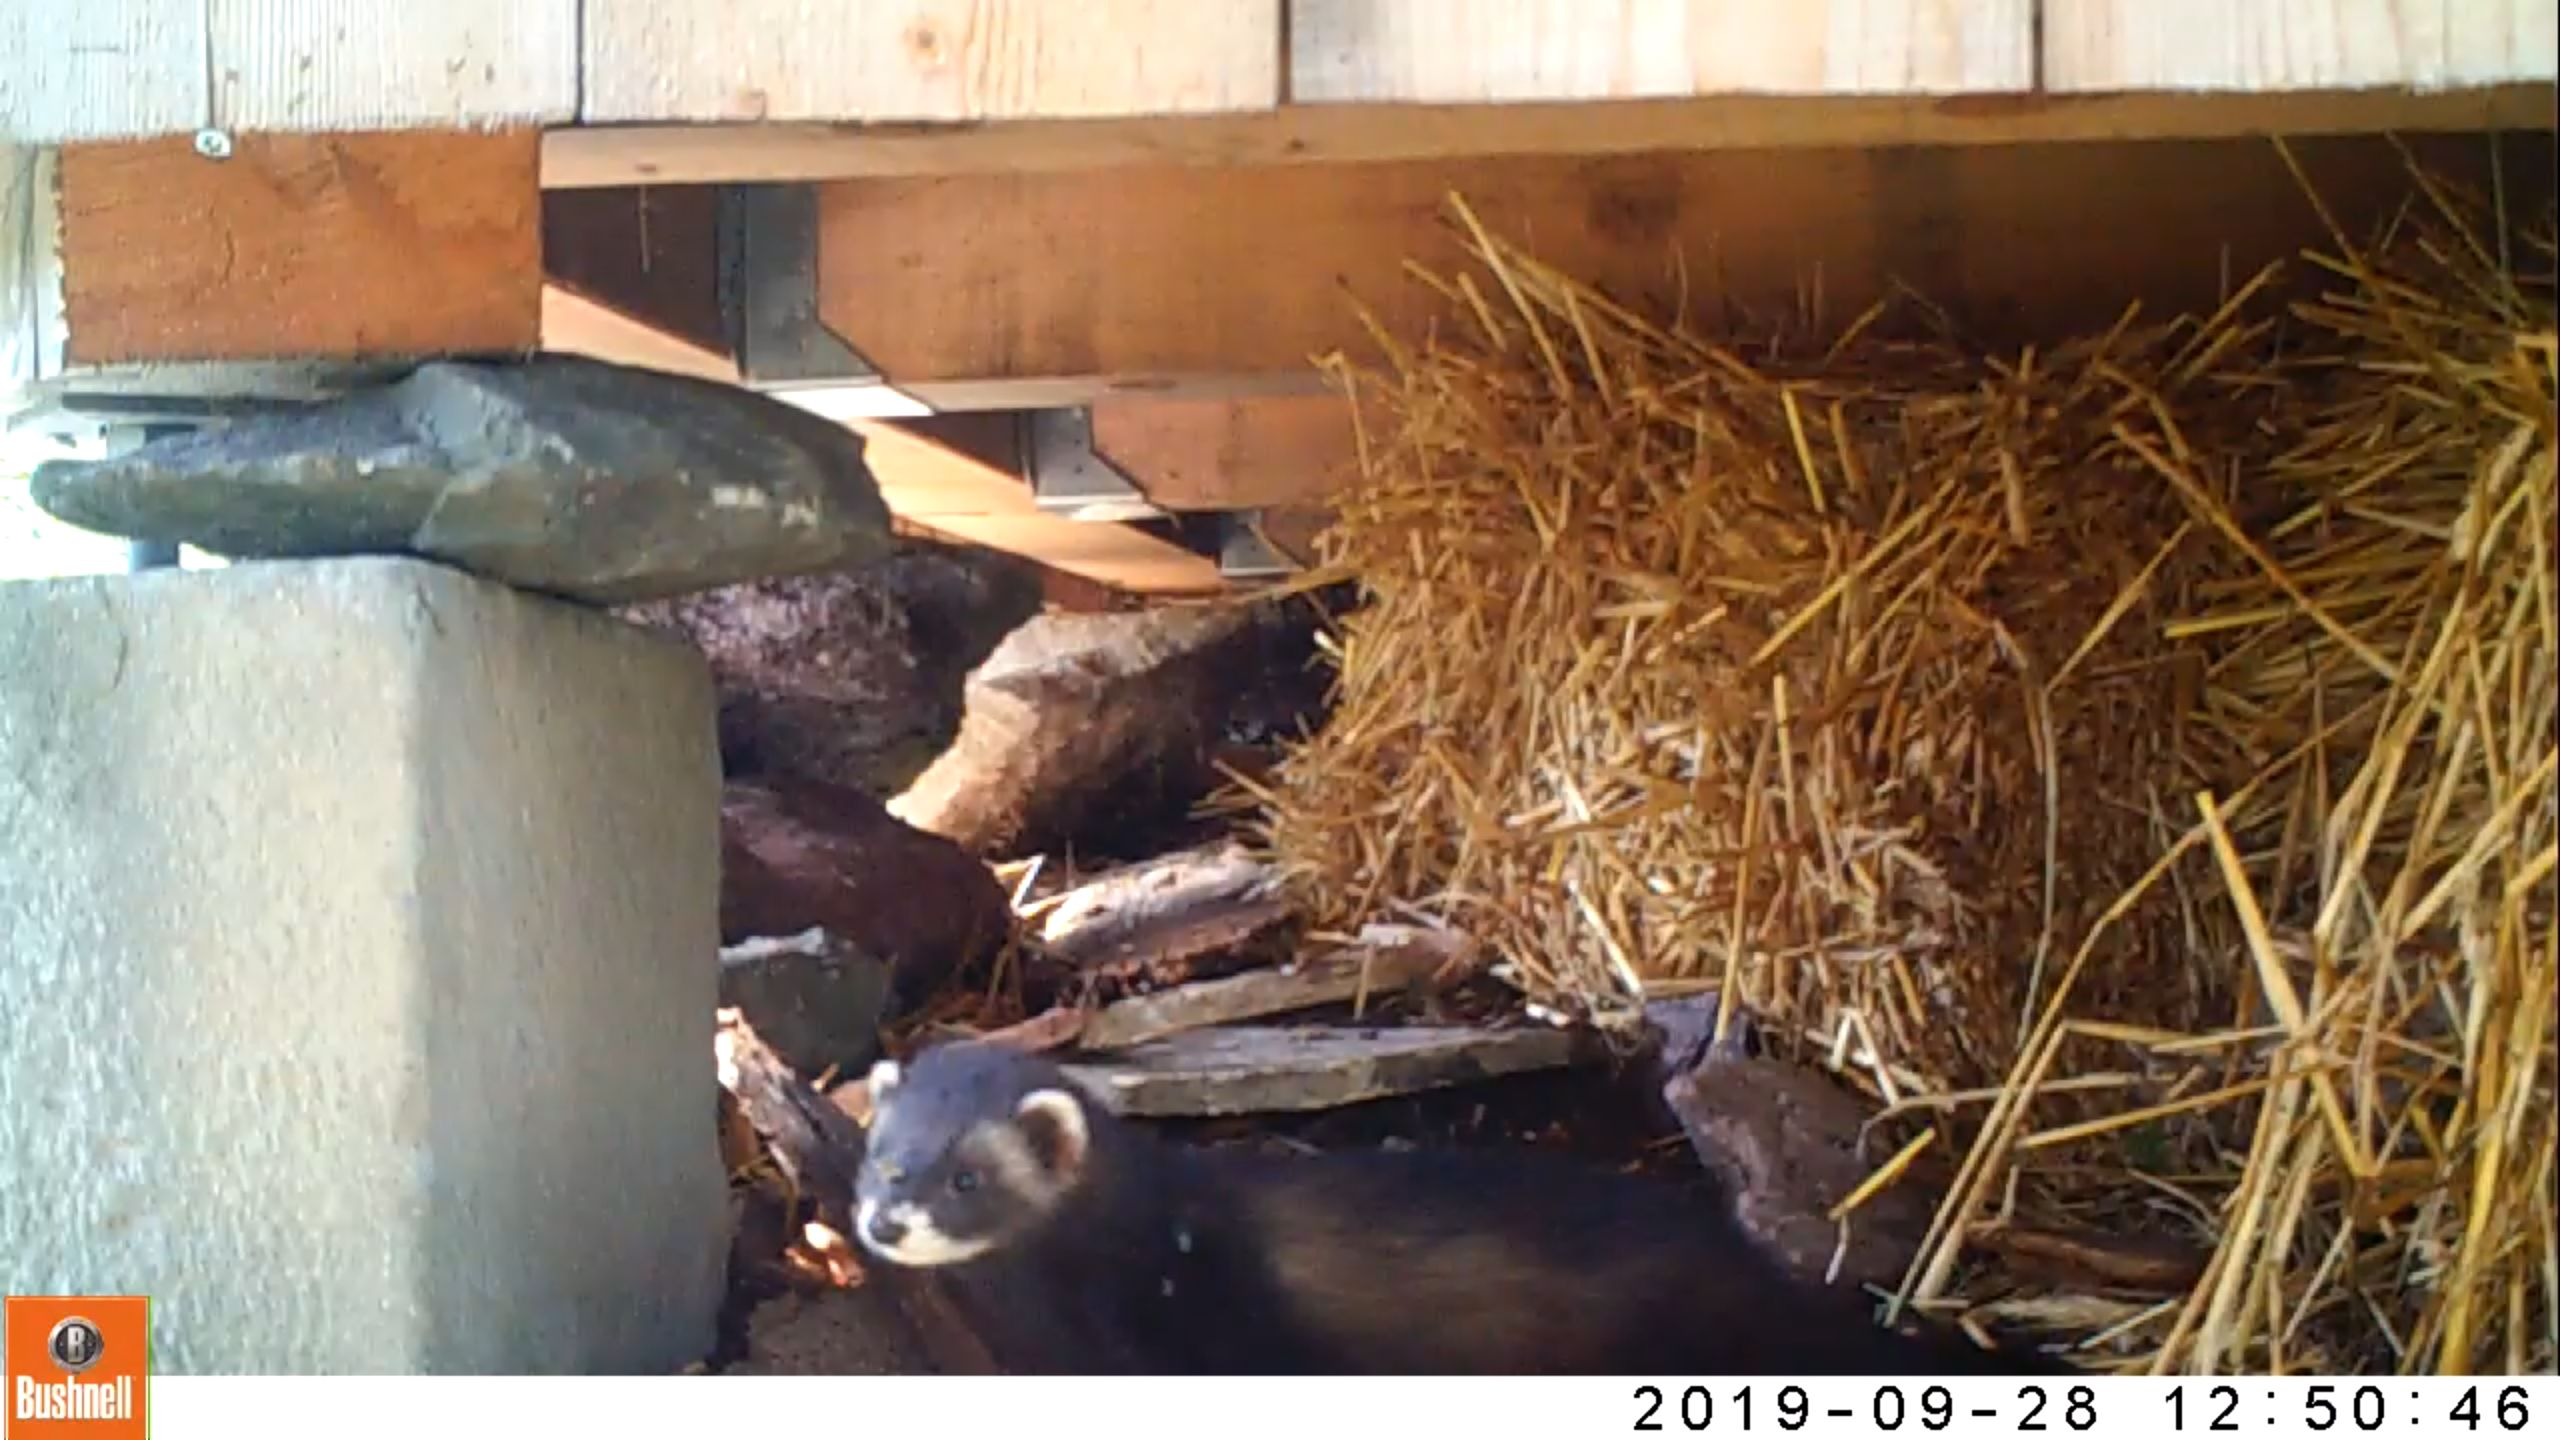
\includegraphics[width=1\linewidth]{images/str13956/capture} \caption{Der Iltis, der meist dämmerungs- und nachtaktiv ist, wurde an einem Winterquartier auch tagsüber (12:50 Uhr, siehe Zeitstempel im Bild) detektiert (Str.13956)}\label{fig:unnamed-chunk-7}
\end{figure}

\begin{figure}[hbt!] \centering 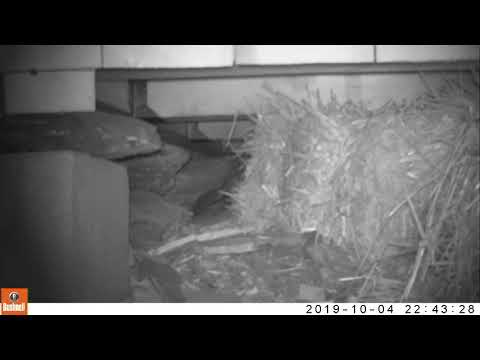
\includegraphics{images/youtube/O5la_63_u_w.jpg} \caption{Der Video ist in voller Länge hier abgespeichert: \url{https://youtu.be/O5la_63_u_w}} \end{figure}\begin{figure}[hbt!] \centering 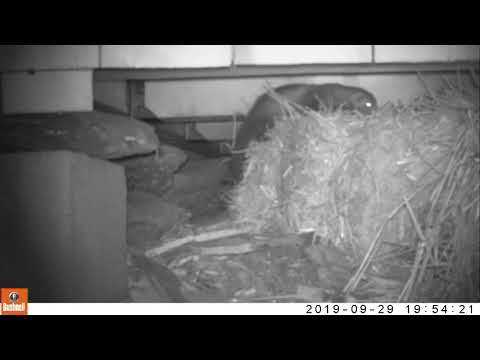
\includegraphics{images/youtube/VCjIpFX3TO0.jpg} \caption{Der Video ist in voller Länge hier abgespeichert: \url{https://youtu.be/VCjIpFX3TO0}} \end{figure}\begin{figure}[hbt!] \centering 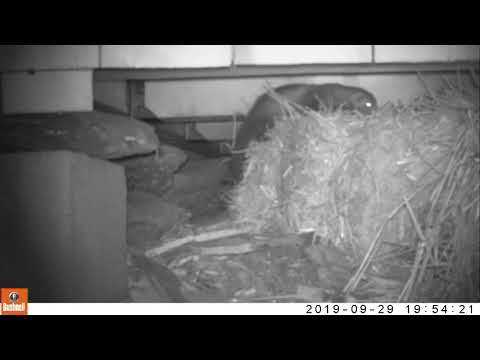
\includegraphics{images/youtube/VCjIpFX3TO0.jpg} \caption{Der Video ist in voller Länge hier abgespeichert: \url{https://youtu.be/VCjIpFX3TO0}} \end{figure}\begin{figure}[hbt!] \centering 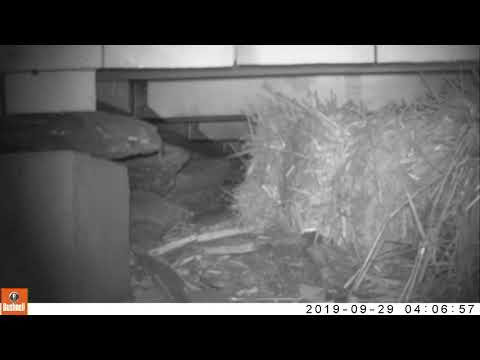
\includegraphics{images/youtube/Hi7ddE5r7B4.jpg} \caption{Der Video ist in voller Länge hier abgespeichert: \url{https://youtu.be/Hi7ddE5r7B4}} \end{figure}\begin{figure}[hbt!] \centering 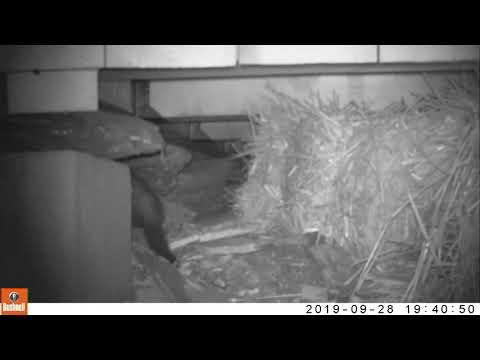
\includegraphics{images/youtube/ISg0ZA5Fvgo.jpg} \caption{Der Video ist in voller Länge hier abgespeichert: \url{https://youtu.be/ISg0ZA5Fvgo}} \end{figure}

\hypertarget{erhebung-3-erhebung-von-asthaufen-eigenschaften-zur-ermittlung-attraktivituxe4tsfuxf6rdernder-faktoren-1}{%
\section{Erhebung 3: Erhebung von Asthaufen Eigenschaften zur Ermittlung attraktivitätsfördernder Faktoren}\label{erhebung-3-erhebung-von-asthaufen-eigenschaften-zur-ermittlung-attraktivituxe4tsfuxf6rdernder-faktoren-1}}

In der Erhebung der Asthaufen Eigenschaften ist bei einer relativ kleinen Stichprobe (25 Asthaufen) für jedes Merkmal zwischen einer relativ hohe Anzahl Kategorien (5 Stufen) unterschieden worden. Dies führt dazu, dass gewisse Merkmalausprägungen unterrepräsentiert sind (z.B. gibt es keine Asthaufen mit der Ausprägung \emph{Astmaterial: sehr fein} oder \emph{benachbarten Kleinstrukturen: sehr wenig}). Dieser Umstand erschwert das Erkennen von Effekten, deshalb werden die 5 Klassen in jeweils 2 Klassen zusammengefasst. Die ursprünglich mittlere Klasse (\texttt{mittel}) wird der jeweils kleineren Klasse zugewiesen in der Bemühung, die beiden neuen Klassen möglichst ausgewogen (gleich gross) zu halten. In Abbildung \ref{fig:asthaufenqualcount} sind die ursprünglichen sowie die neu gebildeten Klassen (farblich gekennzeichnet) ersichtlich.

\begin{figure}
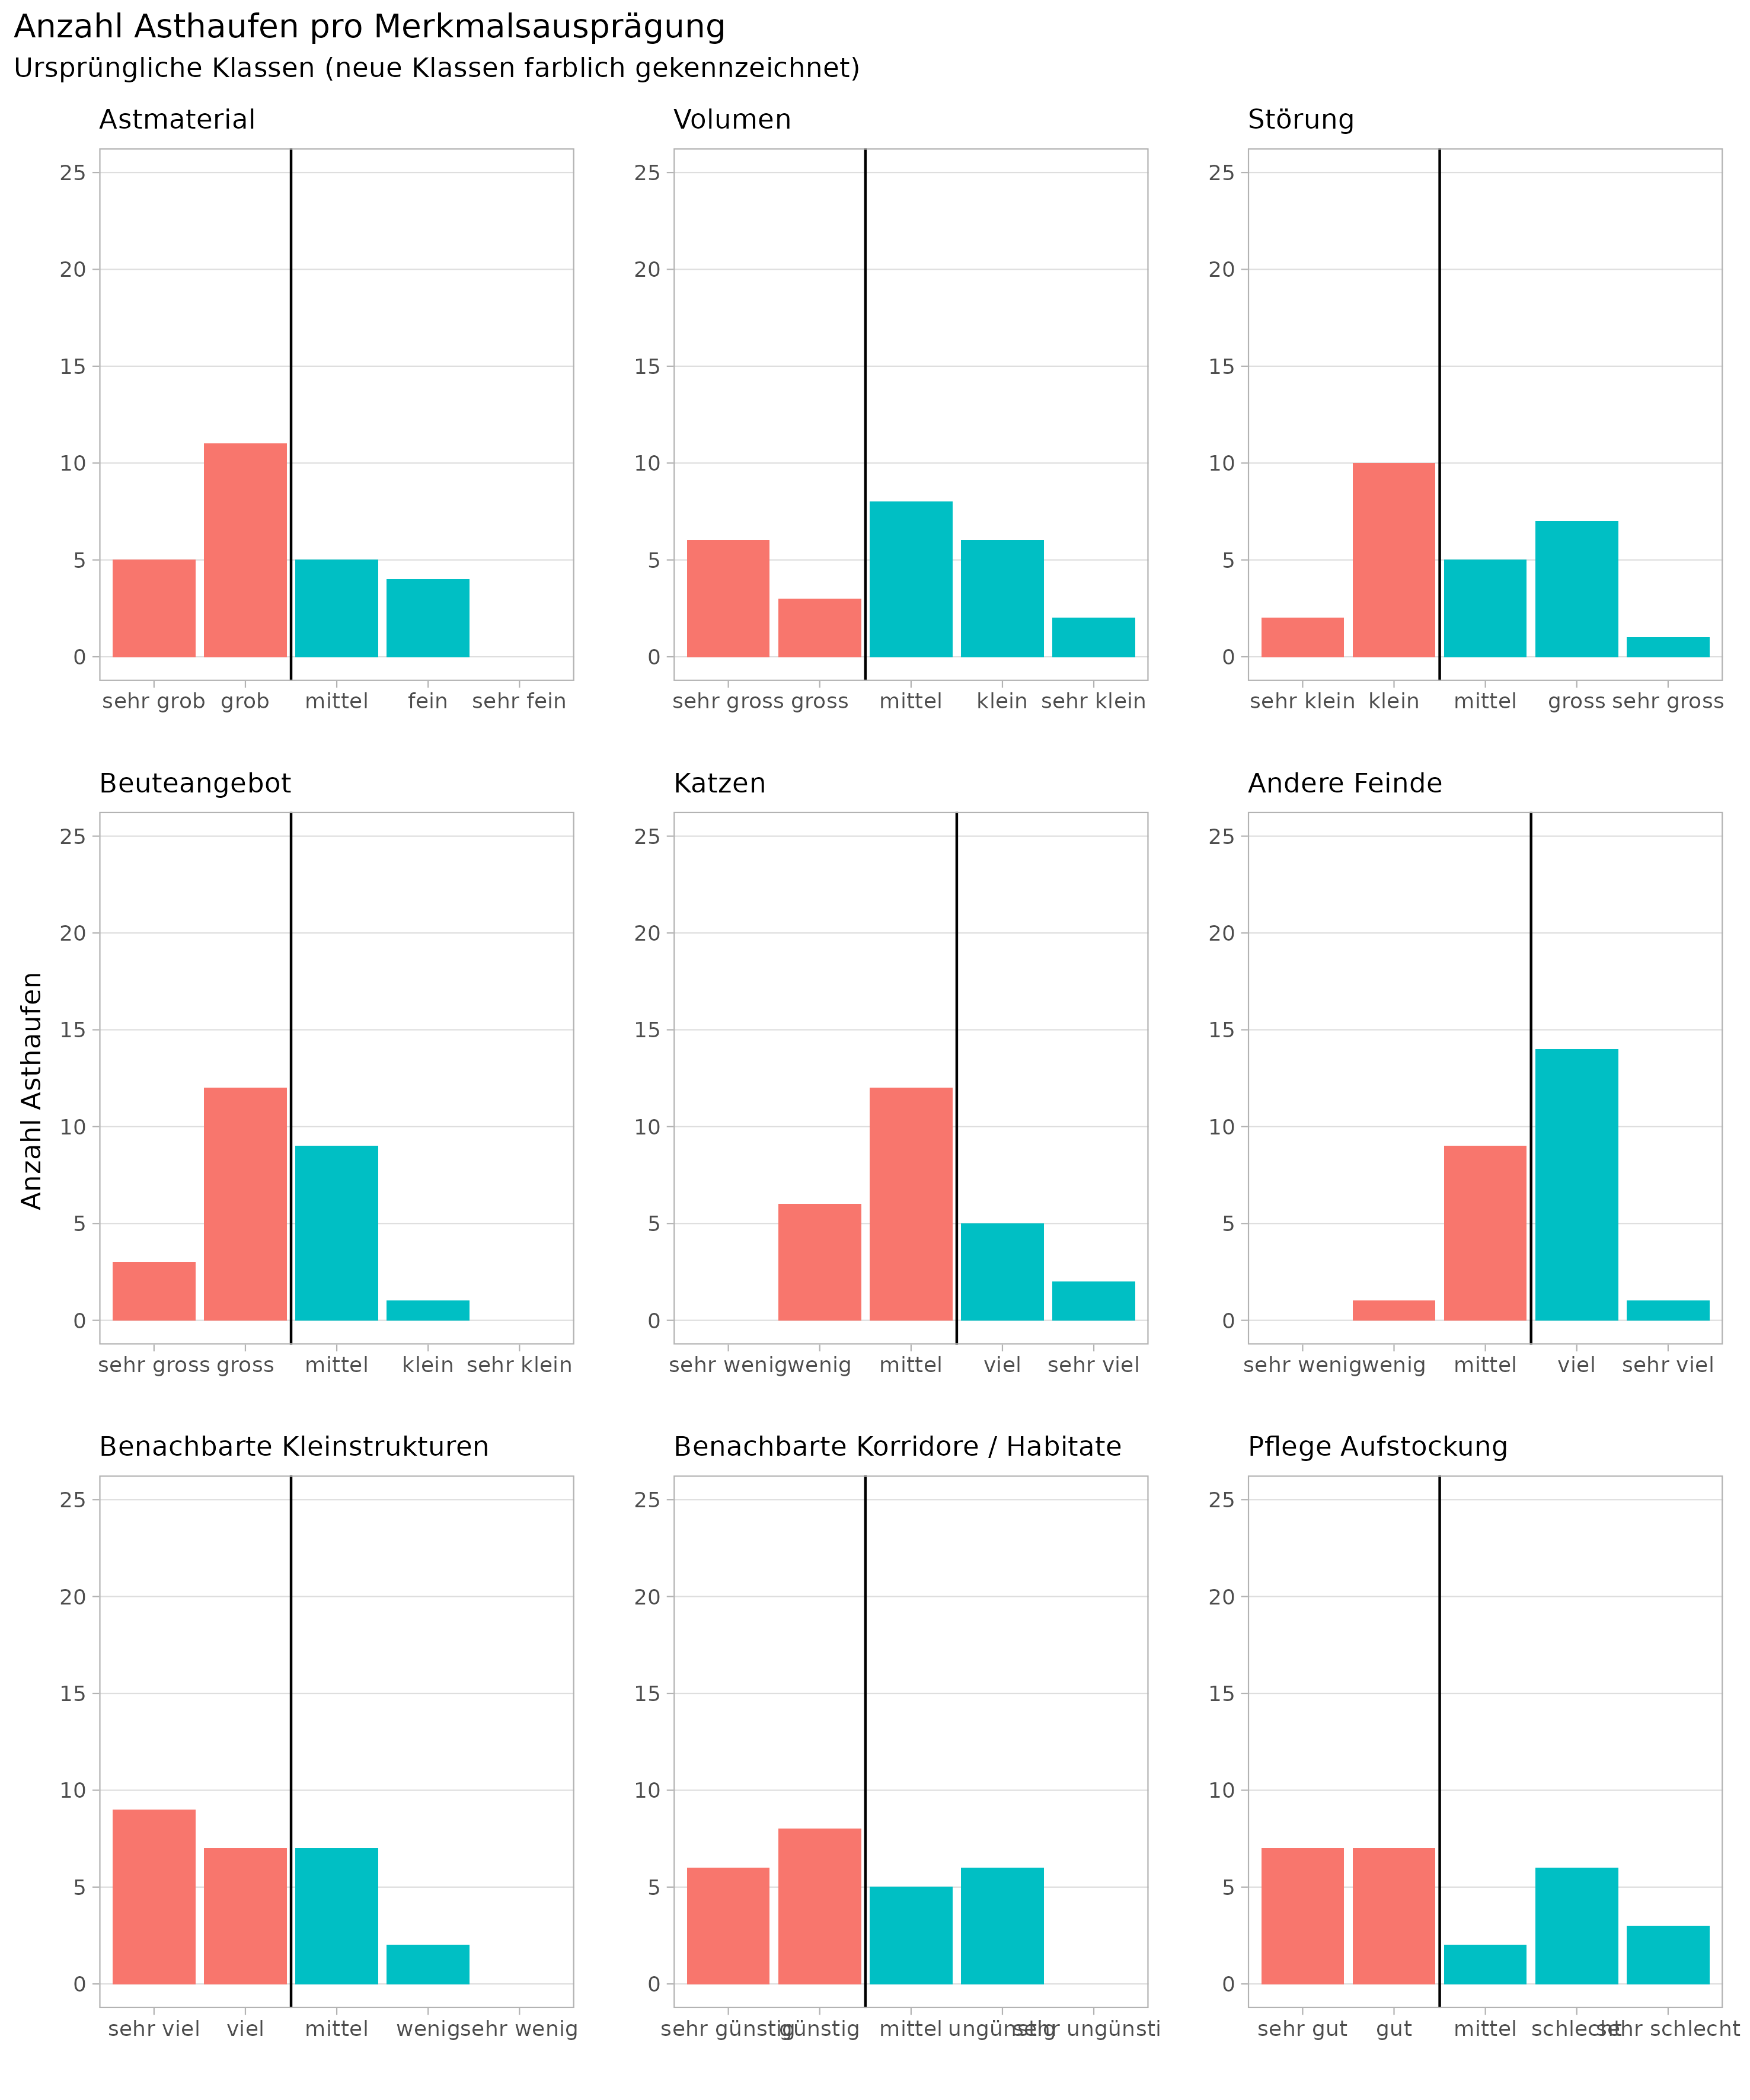
\includegraphics[width=41in]{images/asthaufen_qualitaet_histogramm} \caption{Anzahl Asthaufen pro Merkmalsausprägung}\label{fig:asthaufenqualcount}
\end{figure}

Um den Einfluss der erhobenen Parameter auf die Hermelinbesuche zu prüfen, berechnen wir ein \texttt{poisson} basiertes Generalized Linear Model. Dieses Modell zeigt, dass sich das Hermelinvorkommen durch die Anzahl beanachbarter Korridore (schwach signifikant \texttt{p\ =\ 0.1}, negative Korrelation), vor allem aber durch die Stärke des verwendeten Astmaterials (hoch signifikant, \texttt{p\ =\ 0.01}, positive Korrelation) erklären lässt. Letzteres Resultat besagt, dass die Nachweisquote der Zielarten bei Asthaufen mit einem hohen Bestandteil an grobem Holz hoch signifikant grösser ist.
Der vollständige Modelloutput ist hier ersichtlich:

\begin{verbatim}
## 
## Call:
## glm(formula = total_nach_weise_wk_2019_2020 ~ ., family = "poisson", 
##     data = .)
## 
## Deviance Residuals: 
##     Min       1Q   Median       3Q      Max  
## -1.9579  -0.6978  -0.5812   0.3511   2.1507  
## 
## Coefficients:
##                                  Estimate Std. Error z value Pr(>|z|)   
## (Intercept)                      -0.36079    0.39102  -0.923  0.35617   
## astmaterial.L                     1.58297    0.54235   2.919  0.00351 **
## volumen.L                        -0.02659    0.29225  -0.091  0.92751   
## storung.L                         0.31363    0.37483   0.837  0.40275   
## beute_angebot.L                  -0.23423    0.24796  -0.945  0.34486   
## katzen.L                          0.25120    0.48997   0.513  0.60818   
## andere_feinde.L                   0.13374    0.40013   0.334  0.73819   
## benachbarte_kleinstr.L            0.16059    0.33675   0.477  0.63344   
## benachbarte_korridore_habitate.L -0.55770    0.33119  -1.684  0.09220 . 
## pflege_aufstockung.L             -0.07310    0.39578  -0.185  0.85346   
## ---
## Signif. codes:  0 '***' 0.001 '**' 0.01 '*' 0.05 '.' 0.1 ' ' 1
## 
## (Dispersion parameter for poisson family taken to be 1)
## 
##     Null deviance: 65.194  on 24  degrees of freedom
## Residual deviance: 27.958  on 15  degrees of freedom
## AIC: 86.887
## 
## Number of Fisher Scoring iterations: 6
\end{verbatim}

\hypertarget{datensatz-a-unsystematische-attraktivituxe4tskontrolle-von-asthaufen-1}{%
\section{Datensatz A: Unsystematische Attraktivitätskontrolle von Asthaufen}\label{datensatz-a-unsystematische-attraktivituxe4tskontrolle-von-asthaufen-1}}

In den insgesamt 32 beobachteten Asthaufen konnte das Hermelin 51 und der Iltis 23-mal nachgewiesen werden (siehe Abbildung \ref{fig:wirkungskontrollespontaneinzelnachweisewaffle}): Wie auch schon in der systematischen Wirkungskontrolle, konnte auch in dieser Erhebung das Mauswiesel nicht nachgewiesen werden. Dafür wurde der Iltis einiges häufiger detektiert, in der systematischen Wirkungskontrolle konnten nur zwei Iltisnachweise erbracht werden.



\begin{figure}
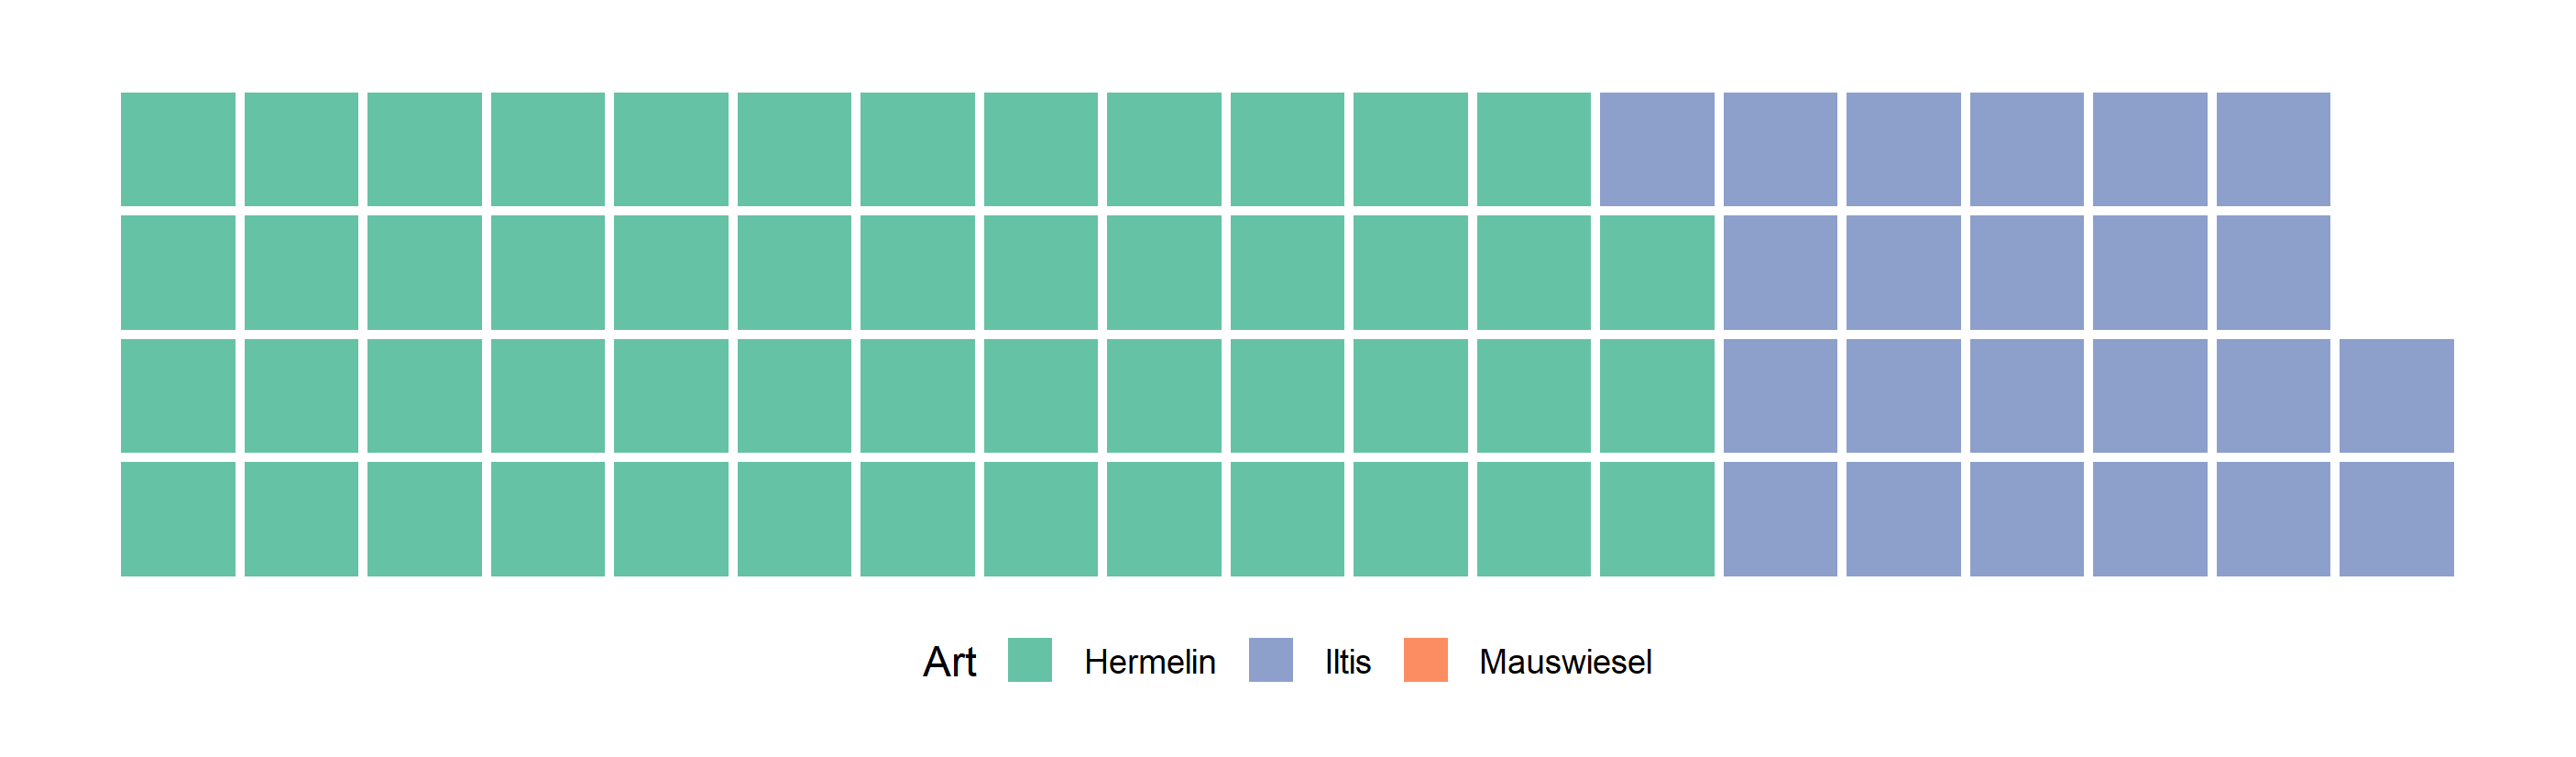
\includegraphics[width=1\linewidth]{images/wirkungskontrolle_spontan_einzelnachweise_waffle} \caption{Zusammenstellung aller Einzelnachweise der Zielarten Hermelin (51 Nachweise), Iltis (23 Nachweise) sowie Mauswiesel (keine Nachweise).}\label{fig:wirkungskontrollespontaneinzelnachweisewaffle}
\end{figure}

Wie bereits erwähnt, kann es sich bei den Einzelnachweisen oft um Mehrfachnachweise des gleichen Individuums handeln. Es ist deshalb sinnvoll, auch den Anteil der Asthaufen mit Nachweisen der Zielart denjenigen ohne Detektion gegenüber zu stellen: In 25 der 32 Asthaufen (78\%) konnte mindestens eine der Zielarten festgestellt werden. In 18 Fällen (60\%) konnte das Hermelin nachgewiesen werden, in 8 Fällen (36\%) der Iltis. In keinem Fall konnte das Mauswiesel in einem Asthaufen nachgewiesen werden.



\begin{figure}
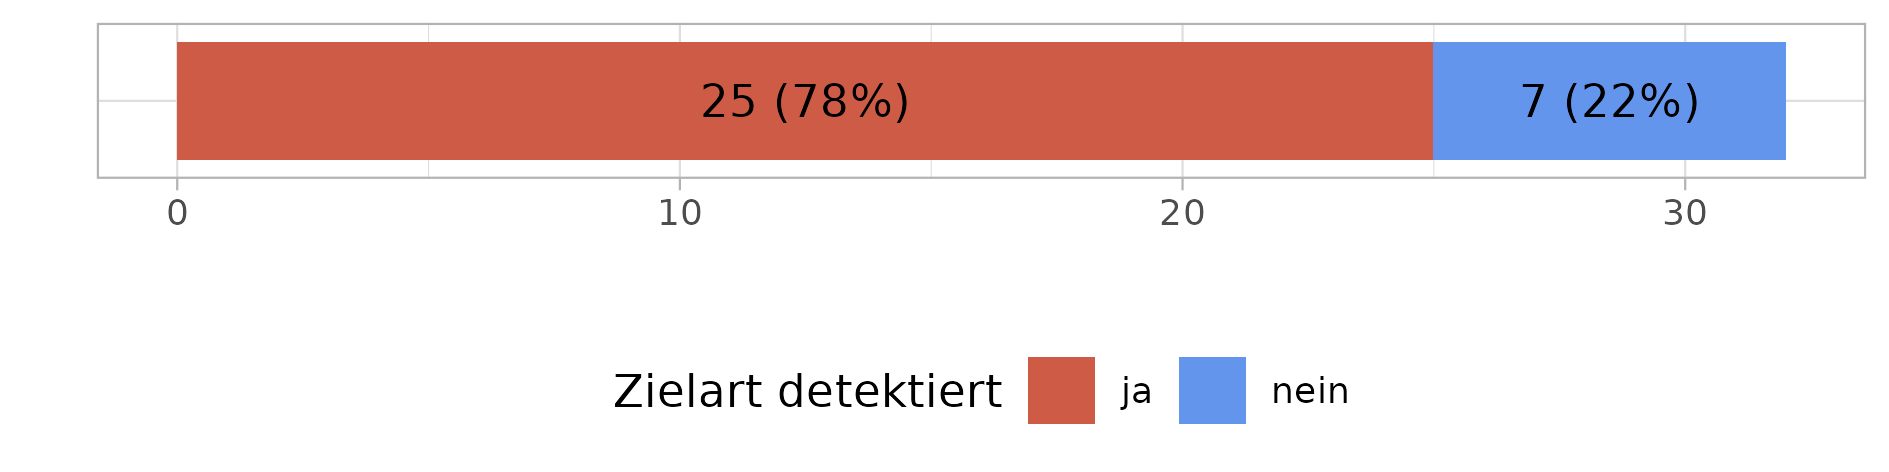
\includegraphics[width=1\linewidth]{images/wirkungskontrolle_spontan_strukturen_mit_zielart} \caption{Anteil der Strukturen, bei dem mindestens eine Zielart nachgewiesen werden konnte.}\label{fig:wirkungskontrollespontanstrukturenmitzielart}
\end{figure}

\hypertarget{datensatz-b-beobachtungsmeldungen}{%
\section{Datensatz B: Beobachtungsmeldungen}\label{datensatz-b-beobachtungsmeldungen}}

Von den 555 Meldungen, die im Projekt gesammelt wurden, handelt es sich bei 546 um Meldungen der Zielarten Hermelin, Iltis und Mauswiesel. Davon wurden 506 Meldungen vom Projektleiter als ``plausibel'' bzw. ``sicher'' eingestuft und davon wiederum liegen 428 Meldungen innerhalb des Projektperimeters, dem Bezirk Horgen (siehe Abbildung \ref{fig:beobachtungsmeldungenfilter}).

Ganz grundsätzlich muss betont werden, dass die Interpretation dieser Meldungen mit einer gewissen Vorsicht gemacht werden muss. Es handelt sich um ein Produkt aus einem ``Citizen Science'' Ansatz, und wie immer liefern solche Datenerzeugnissen ein verzerrtes Bild der Realität. Die Verzerrung entsteht, weil die Meldungen nicht systematisch erfasst und unterschiedliche Räume ungleich intensiv beobachtet werden. Ein Hermelin in einem stark frequentierten und offenen Gebiet hat eine höhere Wahrscheinlichkeit, beobachtet zu werden als ein Tier in einer schlecht frequentierten, strukturreichen Landschaft. Zudem ist davon auszugehen, dass es sich bei sehr dicht beieinanderliegenden Meldungen um Mehrfachmeldungen des gleichen Tiers (womöglich durch den gleichen Beobachter) handelt.

Die grösste Unsicherheit in Bezug auf ihre Plausibilität besteht bei den Mauswiesel-Sichtungsmeldungen. Die Tierart ist aufgrund der geringen Grösse sehr schwer zu beobachten und zudem für Laien kaum vom Hermelin zu unterscheiden. Während lediglich 1.1 \% der Hermelin- und 3.4 \% der Iltismeldungen als ``unsicher'' eingestuft werden, fallen 53.1\% aller Mauswiesel-Sichtungsmeldungen in diese Kategorie. So liegen lediglich 23 verwertbare Mauswiesel-Meldungen vor.



\begin{figure}
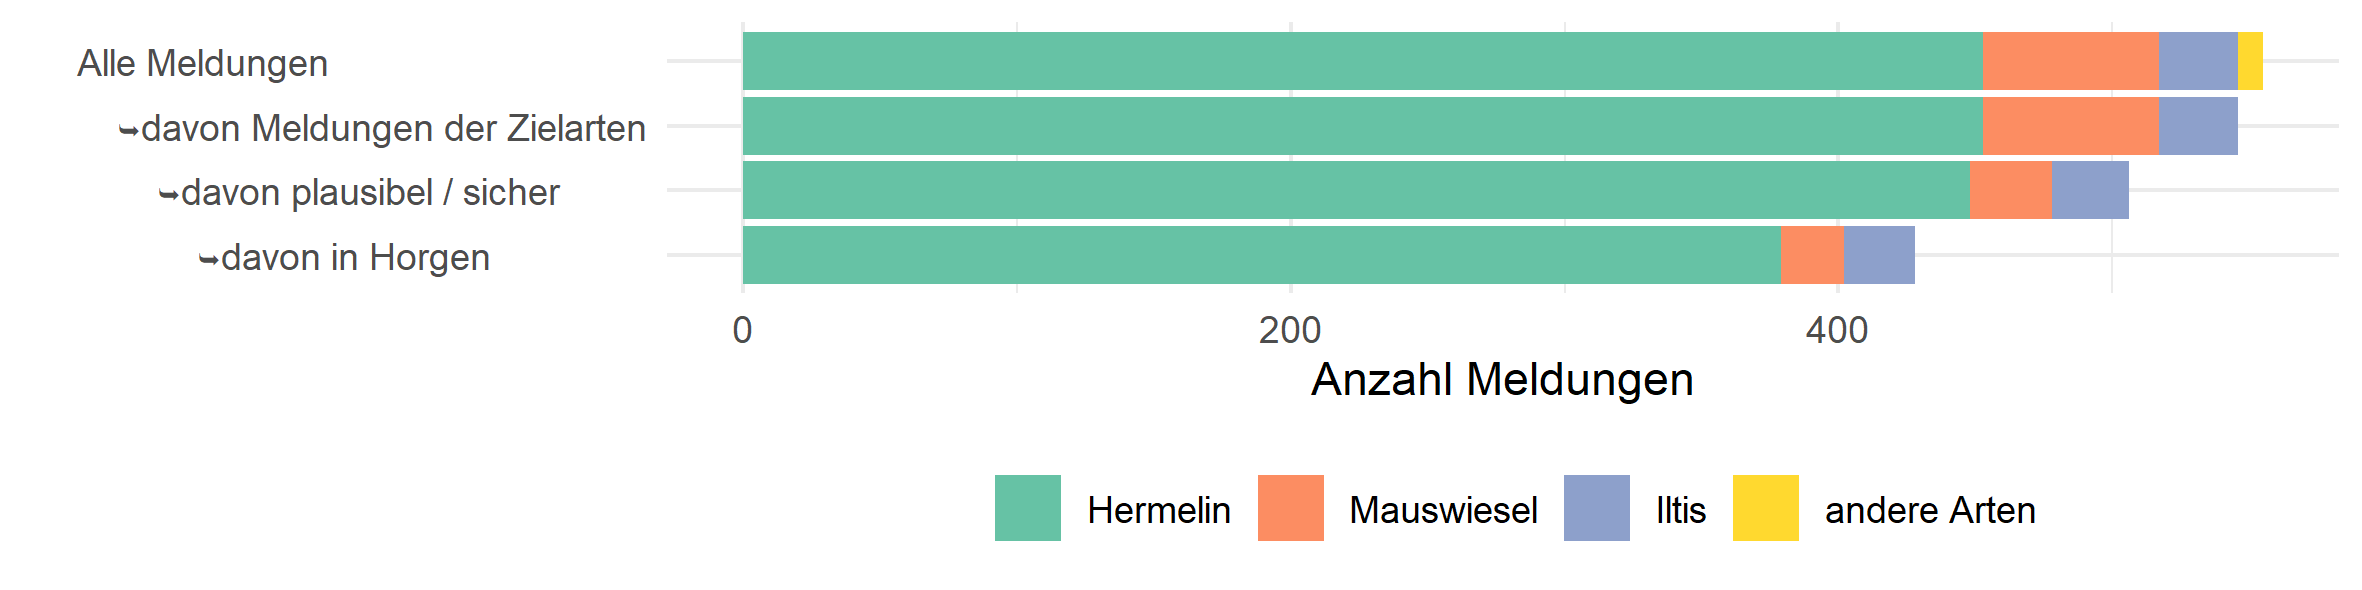
\includegraphics[width=1\linewidth]{images/beobachtungsmeldungen_filter} \caption{Von den 555 Meldungen, die seit Projektbeginn eingetroffen sind, handelt es sich bei 546 Meldungen um die Zielarten, davon können 506 Meldungen als ``plausibel'' bzw. ``sicher'' eingestuft werden. Von diesen Meldungen liegen 428 innerhalb des Bezirks Horgen.}\label{fig:beobachtungsmeldungenfilter}
\end{figure}

Das Hermelin konnte weitestgehend im ganzen Bezirk beobachtet werden, so auch in stark fragmentierten und dicht besiedelten Kulturflächen der Gemeinde Kilchberg und der Halbinsel Au (siehe Abbildung \ref{fig:layoutbeobachtungsmeldungen}). Deutliche Häufungen von Meldungen sind aber in den weniger verbauten Landschaften wie Horgenberg, Hirzel, Schönenberg zu verzeichnen. Weitestgehend ohne Meldungen sind die Siedlungsgebiete selbst sowie der Sihlwald und das Gemeindegebiet Hütten. Während das Fehlen in Siedlungsgebieten und grösseren Waldflächen ökologisch bedingt ist, ist das Ausbleiben von Meldungen in der Gemeinde Hütten mit grösster Wahrscheinlichkeit ein Artefakt davon, dass in Hütten weniger intensiv beobachtet und gemeldet wird.

Deutlich weniger Sichtungsmeldungen sind zum Iltis eingegangen. Dies wiederspiegelt einerseits die tiefere Anzahl Individuen im Vergleich zur Hermelinpopulation, ist aber auch mit Sicherheit der Lebensweise dieser Tierart geschuldet: Als dämmerungs- und nachtaktives Tier, welches sich auch gerne im Waldrandbereich aufhaltet, ist der Iltis seltener zu beobachten als das Hermelin.

Scheinbar willkürlich verteilt sind die Meldungen von Mauswieselsichtungen. Diese sind über den ganzen Bezirk verteilt und ebenfalls nicht auf ein bestimmtes Gebiet konzentriert. Auch zahlenmässig wurde das Mauswiesel sehr viel seltener gesehen als das Hermelin. Dies hängt einerseits sicher mit der erwähnten Schwierigkeit zusammen, Mauswiesel zu beobachten und diese zuverlässig von Hermelinen zu unterscheiden. Es kann aber zusätzlich davon ausgegangen werden, dass die Mauswieselpopulation im Bezirk eher klein und fragil ist.



\begin{figure}
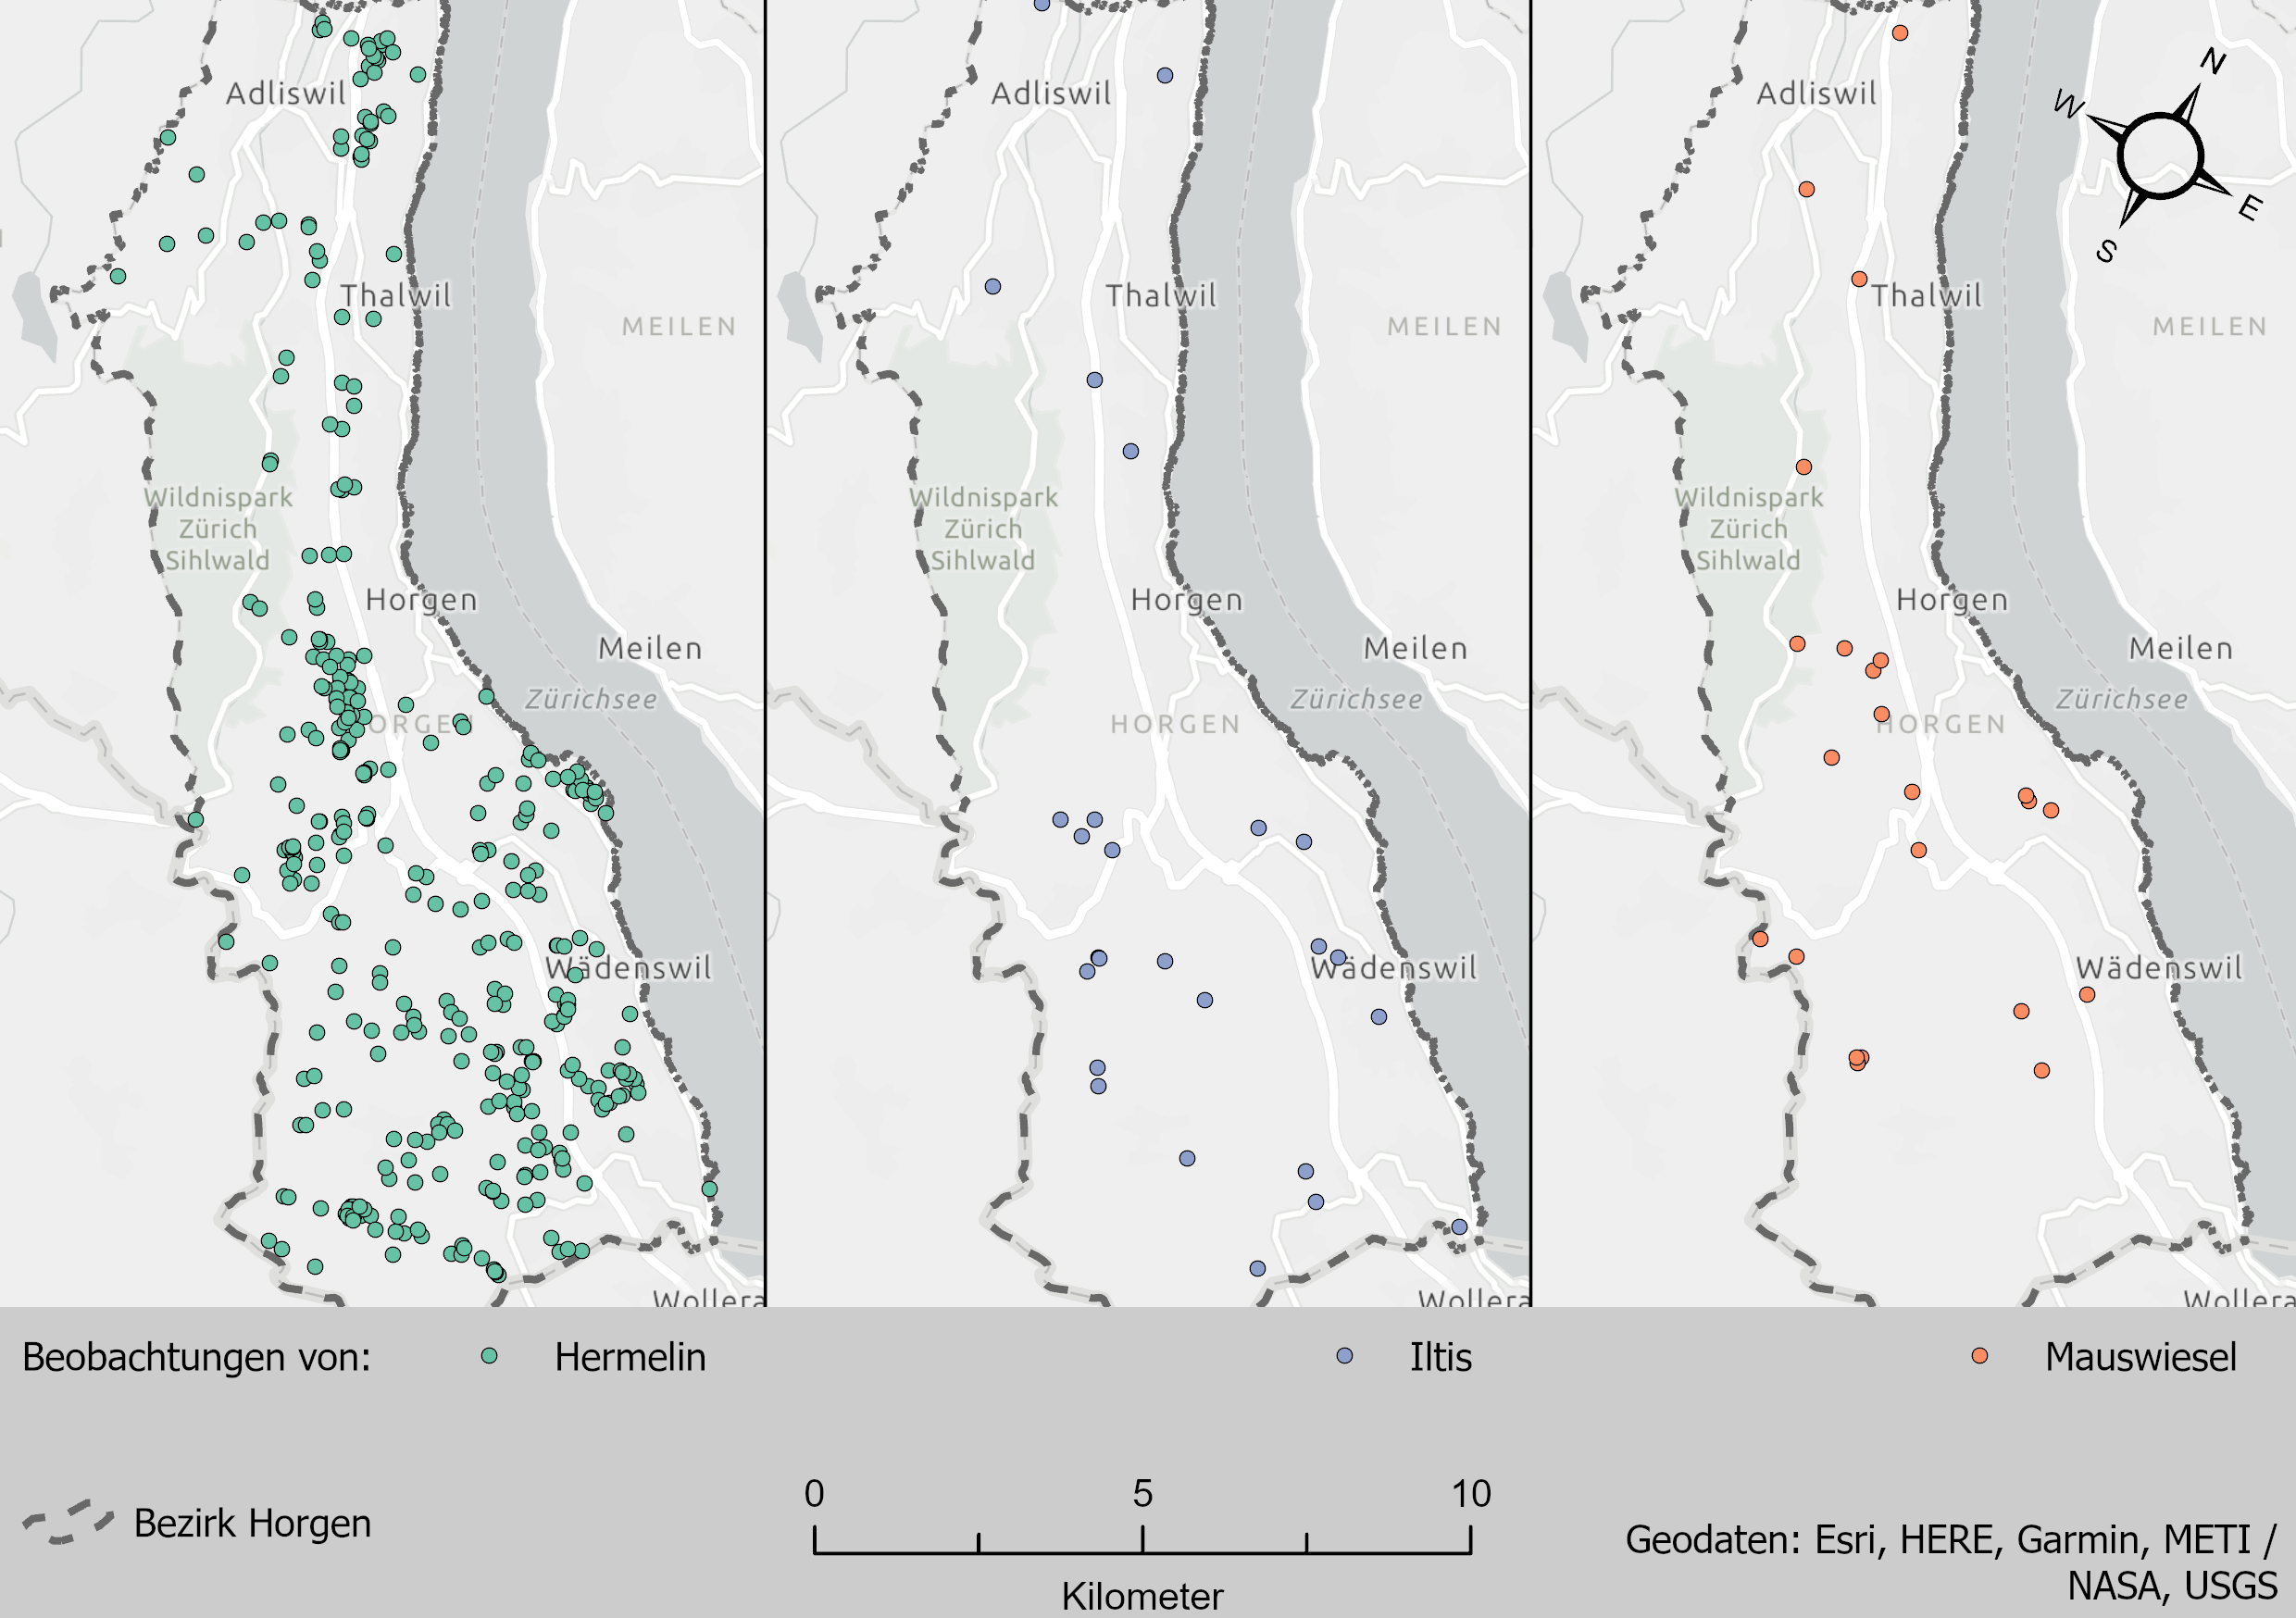
\includegraphics[width=1\linewidth]{images/Layout_Beobachtungsmeldungen} \caption{Beobachtungsmeldungen der Zielarten Hermelin, Iltis und Mauswiesel im Bezirk Horgen.}\label{fig:layoutbeobachtungsmeldungen}
\end{figure}

\hypertarget{diskussion-und-fazit}{%
\chapter{Diskussion und Fazit}\label{diskussion-und-fazit}}

\hypertarget{vergleich-mit-den-zielsetzungen-von-win-wieselnetz}{%
\section{Vergleich mit den Zielsetzungen von WIN Wieselnetz}\label{vergleich-mit-den-zielsetzungen-von-win-wieselnetz}}

Müri und Weinberger (2015) legen für Projekte im Rahmen von ``Wiesellandschaft Schweiz'' der Stiftung WIN Wieselnetz Ziele fest, um Erfolgskontrollen quantitativ messen zu können. Dabei wird davon ausgegangen, dass Spurentunnel jeweils beködert werden. Sollte diese Beköderung nicht stattfinden, müssten die Ziele gemäss dem Bericht ``nach unten angepasst werden'' (Müri und Weinberger, 2014).

In der vorliegenden Untersuchung wurde auf eine Beköderung verzichtet. In diesem Sinne wurden die Ziele für die vorliegende Wirkungskontrolle folgendermassen adaptiert: Anstatt dass die Ziele für jedes Jahr getrennt beurteilt werden, werden die Daten aus beiden Jahren zusammen geführt und über beide Jahre beurteilt (siehe Tabelle \ref{tab:winziele}). Dieser Ansatz trägt auch den starken Schwankungen in den Wieselpopulationen Rechnung.

\begin{table}

\caption{\label{tab:winziele}Zieldefinition in Anlehnung an Müri und Weinberger (2014) sowie ihre Beurteilung und Bemerkungen.}
\centering
\begin{tabular}[t]{rp{65mm}>{}lp{60mm}}
\toprule
Nr & Zieldefinition & Beurteilung & Bemerkung\\
\midrule
\cellcolor{gray!6}{1} & \cellcolor{gray!6}{In jedem Populationsraum sollen zu jeder Kontrollperiode Mauswiesel und Hermelin nachgewiesen werden.} & \cellcolor{gray!6}{}
\includegraphics[width=0.67in, height=0.24in]{images/ampel_gelb.png} & \cellcolor{gray!6}{Es konnten zwar Hermeline, aber keine Mauswiesel nachgewiesen werden.}\\
2 & Mind. 50 \% der aufgewerteten Kleinstrukturen sollen von Wieseln (Hermelin oder Mauswiesel) begangen werden. & 
\includegraphics[width=0.67in, height=0.24in]{images/ampel_gelb.png} & Bei getrennter Betrachtung der Jahre: 49 \% resp. 36 \%. Kumulativ über beide Jahre: knapp 70 \%\\
\cellcolor{gray!6}{3} & \cellcolor{gray!6}{In mind. 75 \% der untersuchten Patches1 des Populationsraums sollen Nachweise von Hermelinen erbracht werden.} & \cellcolor{gray!6}{}
\includegraphics[width=0.67in, height=0.24in]{images/ampel_gruen.png} & \cellcolor{gray!6}{In 10 von 11 untersuchten Patches (91 \%) konnten Nachweise von Hermelinen erbracht werden.}\\
4 & In mind. 25 \% der untersuchten Patches1 des Populationsraums sollen Nachweise von Mauswieseln erbracht werden. & 
\includegraphics[width=0.67in, height=0.24in]{images/ampel_rot.png} & In Erhebung 1 konnten keine Mauswiesel3 nachgewiesen werden.\\
\cellcolor{gray!6}{5} & \cellcolor{gray!6}{In jeder untersuchten Verbindungsachse sollen mindestens einmal pro Jahr Wiesel (mindestens Hermeline) nachgewiesen werden.} & \cellcolor{gray!6}{}
\includegraphics[width=0.67in, height=0.24in]{images/ampel_gelb.png} & \cellcolor{gray!6}{Gemäss Datensatz A2 konnten auf 4 von 5 kontrollierten Korridoren Nachweise von Hermelin und Iltis gemacht werden}\\
\bottomrule
\end{tabular}
\end{table}

Der Zielvergleich fällt folgendermassen aus: Ein Ziel wurden erreicht (Ziel 3), drei Ziele wurden teils erreicht (Ziel 1, 2 und 5) und ein weiteres Ziel konnte nicht erreicht werden (Ziel 4). Grund für die Nicht- bzw. Teilerreichung der Ziele 1 und 4 ist das Fehlen von Mauswieselnachweisen in Erhebung 1 (Systematische Beobachtung der Asthaufen). Dabei ist jedoch zu betonen, dass der Nachweis bei kleinen, fragilen Populationen ungleich schwieriger zu erbringen ist als in Gebieten mit höherem Mauswiesel Vorkommen. Das Projekt hat, insbesondere in der kurzen Laufzeit, nur einen kleinen Einfluss auf die Mauswiesel-Populationsstärke. In diesem Sinne ist das Teilerreichen der Ziele 1 und 5 nicht durch Fehler im Projekt zu erklären, sondern vielmehr eine ökologische Gegebenheit.

\hypertarget{nachweisquote-im-vergleich-mit-anderen-studien}{%
\section{Nachweisquote im Vergleich mit anderen Studien}\label{nachweisquote-im-vergleich-mit-anderen-studien}}

Der Austausch mit Projektleitern und Ökologen anderer Wieselprojekte in der Schweiz zeigt, dass die gesetzten Nachweisziele von WIN Wieselnetz (Tabelle \ref{tab:winziele}) sehr hoch gesteckt sind. Aus diesem Grund wurden die Resultate anderer Studien zusammengetragen und in Abbildung \ref{fig:kontext} visualisiert. Dargestellt sind die ``Nachweiserfolge'' von verschiedenen Studien, definiert als der Anteil der Spurentunnel, die mindestens einen Hermelinnachweis erbracht haben. Die Abbildung macht deutlich, dass die vorliegende Studie einen sehr hohen Nachweiserfolg zu verzeichnen hat.
Der Anteil der Spurentunnel mit Hermelinnachweisen im Vergleich zur totalen Anzahl eingesetzter Spurentunnel ist ausserordentlich hoch und liegt bei 49 \% (2019) bzw. 36 \% (2020).
Das Ergebnis der unsystematischen Wirkungskontrolle (Datensatz B, siehe @ref(\#methode-datensatz-b)) hebt sich noch stärker von anderen Untersuchungen ab, wobei die methodischen Eigenschaften (insbesondere die langen Kontrollperioden), die Vergleichbarkeit einschränken.

Eine Erklärungsmöglichkeit für die hohen Nachweisquoten ist die grosse Dichte an Schermäusen, welche eine vorzügliche Nahrungsgrundlage für Hermeline (und Mauswiesel) bildet. Die hinzukommenden Kleinstrukturen in der streckenweise strukturarmen Zimmerberglandschaft üben eine starke Anziehungskraft aus. Wären viele andere Kleinstrukturen vorhanden, könnte der Nachweiserfolg kleiner sein, auch wenn zugleich die Hermelinpopulation grösser wäre.



\begin{figure}
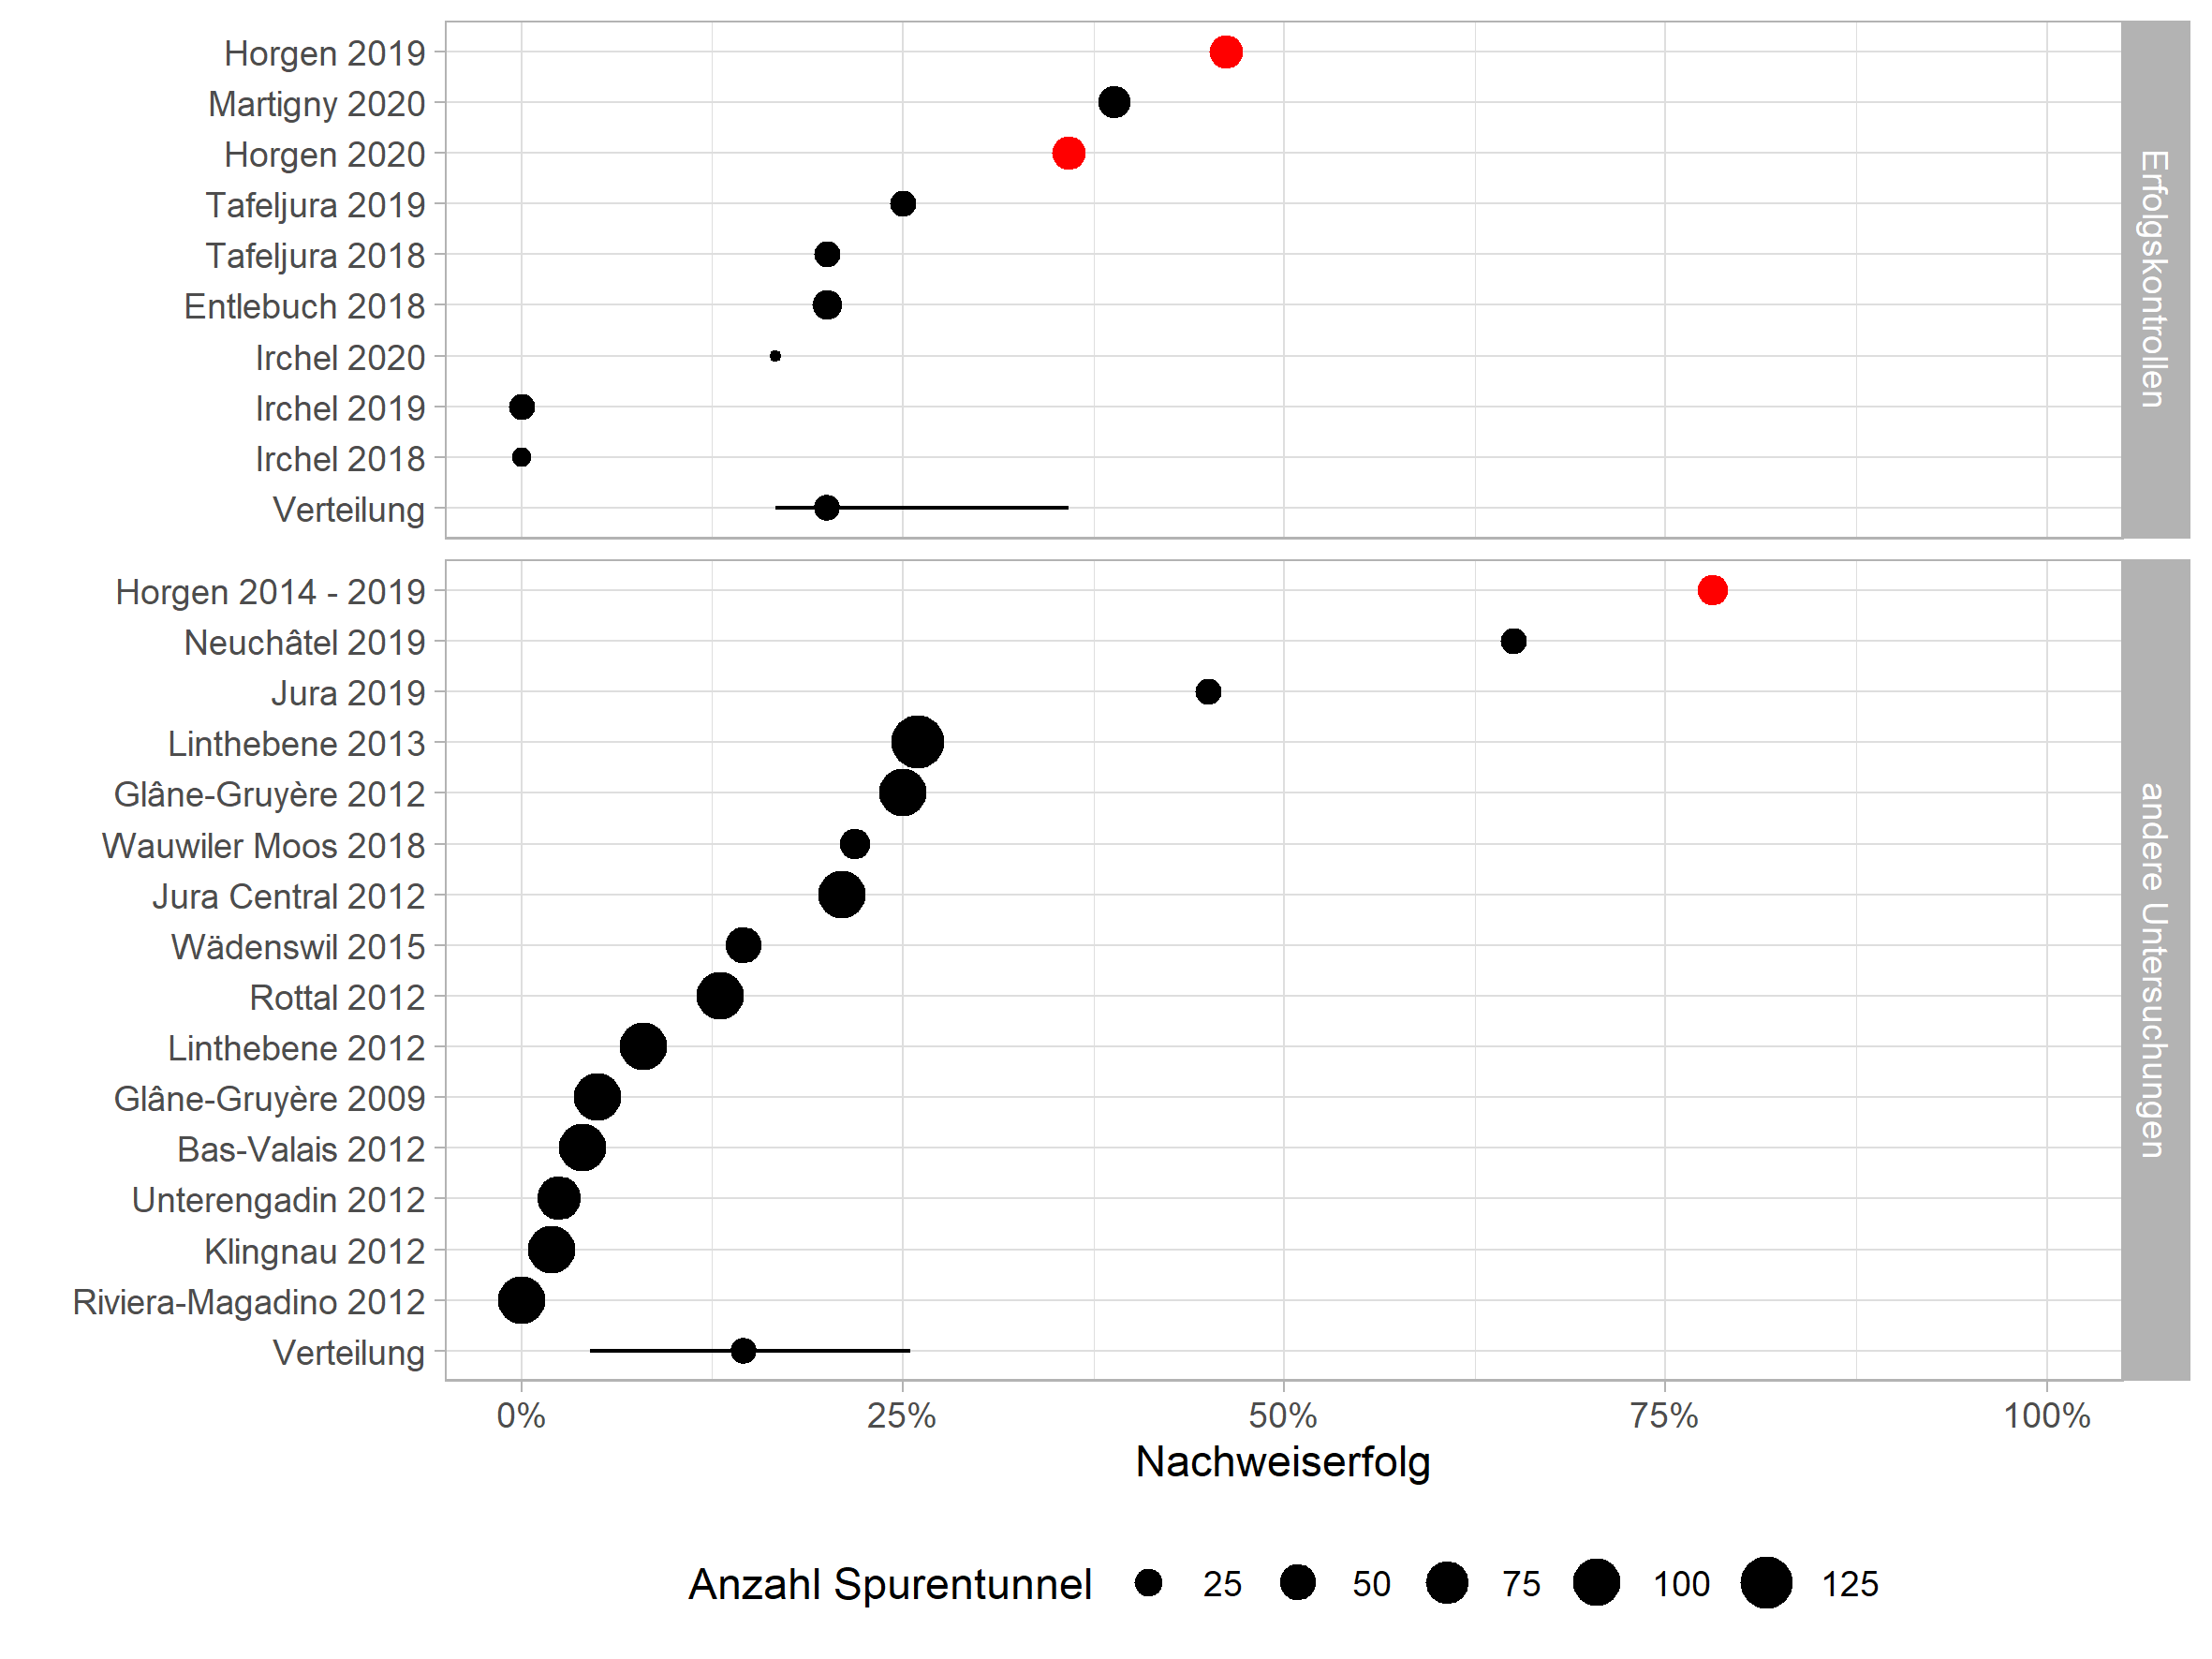
\includegraphics[width=1\linewidth]{images/kontext} \caption{Der Nachweiserfolg aus Spurentunneluntersuchungen anderer Studien (für Quellenangaben siehe Anhang \ref{anhang-zusammenstellung})}\label{fig:kontext}
\end{figure}

\hypertarget{interpretation-der-nachweiszahlen}{%
\section{Interpretation der Nachweiszahlen}\label{interpretation-der-nachweiszahlen}}

\hypertarget{hermlin-vs.-mauswiesel}{%
\subsection{Hermlin vs.~Mauswiesel}\label{hermlin-vs.-mauswiesel}}

Die Nachweiszahlen zeigen, dass das Hermelin am Zimmerberg die deutlich häufigste der drei Zielarten ist. Datensatz B zeigt bei den Beobachtungsmeldungen ca. ein Verhältnis von 1 Mauswiesel und 1 Iltis auf 20 Hermeline.
Gegenüber 59 Hermelinnachweisen während der Wirkungskontrolle wurde der Iltis 5 Mal nachgewiesen und das Mauswiesel wurde nur 1 Mal mit Spurentunnel ausserhalb der regulären Wirkungskontrolle festgestellt.

\begin{table}

\caption{\label{tab:unnamed-chunk-11}Summe der Nachweise je Tierart in Erhebung 1 (Asthaufen) und 2 (Winterquartiere)}
\centering
\begin{tabular}[t]{l|r|r|r}
\hline
typ & Hermelin & Iltis & Mauswiesel\\
\hline
Asthaufen & 55 & 2 & 0\\
\hline
Winterquartiere & 4 & 3 & 0\\
\hline
\end{tabular}
\end{table}

Bei vergleichbaren Wirkungskontrollen ist nach Meinung von Experten ein Nachweisverhältnis von 1 Mauswiesel auf 5 Hermeline für die Schweiz durchschnittlich (Simon Capt mündliche Mitteilung).
Zwei Gründe könnten für das Mauswiesel ungünstigere Verhältnis verantwortlich sein.

\begin{itemize}
\tightlist
\item
  \textbf{Dominanz des Hermelin aufgrund der idealen Nahrungsgrundlage}: Die grossen Schermausbestände in der grünlandbasierten Zimmerberglandschaft sind vom Hermelin effizient zu bejagen. Das schwächere Mauswiesel zieht sich bei Anwesenheit des Hermelins an Orte mit kleineren Wühlmausarten zurück, die sich vor allem auf Nischenvorkommen wie Feuchtgebieten, kleinräumigen Halboffenlandschaften etc. beschränken.
\item
  \textbf{Benachteiligung des Mauswiesels durch mangelnde Kleinräumigkeit bzw. Vernetzung}: Das Mauswiesel hat einen kleineren Aktionsradius und die vorherrschende Lebensraumqualität erschwert ihm, auf kleinem Raum zugleich geeignete Nahrung, genügend Deckung und funktionale Vernetzungskorridore zu finden. Gleichzeitig dürfte es gegenüber dem Hermelin noch anfälliger gegenüber Katzen und anderen Feinden sein.
\end{itemize}

Diese Gründe sind allerdings mit einiger Unsicherheit belegt, und auch nach Durchführung des Projekts ist über die Populationsdynamik im Bezirk Horgen nicht viel bekannt. Das Projekt hat aber einige sichere Mauswiesel-Beobachtungen hervorgebracht und zur Weiterentwicklung effektiverer Methoden für den Nachweis von Mauswieseln und anderen Kleinsäugern beigetragen (siehe \href{https://www.zhaw.ch/iunr/tubecam}{zhaw.ch/iunr/tubecam} und \href{http://wieselundco.ch/wissenschaft}{wieselundco.ch/wissenschaft}).

\hypertarget{iltis}{%
\subsection{Iltis}\label{iltis}}

Bei den Iltisnachweisen fällt auf, dass diese in 3 von 5 Fällen von Winterquartieren in Streuhütten stammen. Es bestätigt sich also, dass dieser Massnahmentyp hauptsächlich dem Iltis zu Gute kommt. Wahrscheinlich einerseits aufgrund der Bindung an Feuchtlebensräume und andererseits wegen des vorzüglichen Witterungsschutzes solcher Objekte. Insofern kann mit den Winterquartieren ein Beitrag zur Iltisförderung geleistet werden, die durch Weber (1989) inspiriert wurde.

\hypertarget{erkenntnisse-fuxfcr-die-anlagen-von-asthaufen}{%
\section{Erkenntnisse für die Anlagen von Asthaufen}\label{erkenntnisse-fuxfcr-die-anlagen-von-asthaufen}}

Interessant ist die Erkenntnis, dass grobes Material bei Holzstrukturen die Attraktivität zu fördern scheint. Nebst der guten Zugänglichkeit dürfte ein weiterer Grund die vorteilhafte Bekletterbarkeit und damit die Ermöglichung des räumlichen Überblicks zur Feindvermeidung sein.
Idealerweise wird ein Asthaufen von Beginn weg aus grobem, massivem Material wie Wurzelstöcken, Stamm- und Stangenholz aufgebaut - bestenfalls aus beständigen Holzarten. Denn die realisierten Asthaufen sollen auch möglichst lange bestehen. Zu bedenken ist, dass selbst voluminöse Asthaufen innert weniger Jahren stark zerfallen, sofern sie aus Weichholz aufgebaut werden. Diesem Zerfall kann mit einer periodischen Aufstockung begegnet werden.
Um die Nachaltigkeit zu fördern, wurde das Knowhow mit persönlicher Beratung und anlässlich Dutzender Aktionstage interessierten Landwirtinnen und weiteren interessierten Personen vermittelt. Zudem gaben die zweijährlich wiederkehrenden Vergütungen Anreiz für Pflegemassnahmen.

\hypertarget{fazit-und-ausblick}{%
\section{Fazit und Ausblick}\label{fazit-und-ausblick}}

Es muss davon ausgegangen werden, dass die sich immer mehr ausbreitende ``Normallandschaft'' im Schweizer Mittelland nicht nur bei Artengruppen wie Vögeln, sondern auch bei Kleinraubtieren die Generalisten gegenüber den Spezialisten begünstigt. So könnte das im Mittelland ohnehin seltenere Mauswiesel zukünftig grossräumig in seiner Existenz gefährdet sein. Es scheint, dass eine kleinräumigere Landschaft mit einer extensiver betriebenen Landwirtschaft den Bestand des Mauswiesel gegenüber jenem des Hermelins vergrössern könnte. Davon würde dank verbesserten Deckungsmöglichkeiten und Nahrungsgrundlagen wahrscheinlich auch der Iltis profitieren.

Dahingehende Fördermassnahmen, die im Rahmen des Projektes realisiert wurden, werden von zwei der drei Zielarten nachweislich stark frequentiert. Diese Tatsache wiederspiegelt die sinnvolle Planung und Umsetzung der Strukturen. Es existieren nach unserem Wissen wenige Projekte in der Schweiz, die eine solch hohe Anzahl an Asthaufen zur Förderung von Kleinraubtieren erstellt wurden.

Das Projekt Wiesel \& Co am Zimmerberg hat einen nennenswerten Beitrag zur Förderung der Tierarten im Bezirk Horgen geleistet. In sozialer Hinsicht ist es der Trägerschaft gelungen, die Kräfte aller lokalen Naturschutzvereine zu bündeln und den Kontakt zu zahlreichen Landwirten*innen, Jäger*innen, Förster*innen, Schulklassen und Freiwilligen zu finden und die Sensibilisierung für die Zielarten zu fördern. Aus ökologischer Hinsicht ist die Umsetzung einer beachtlichen Anzahl von Aufwertungsmassnahmen gelungen, welche nachweislich durch zwei der drei im Projekt festgesetzten Tierarten genutzt wurden.

Für eine langfristige Sicherstellung von Naturschutzmassnahmen ist die Projektträgerschaft bemüht, das Projekt nach Abschluss in eine langfristige, breit abgestützte Form zu überführen. Dazu wurde 2020 die Initiative Naturnetz Zimmerberg lanciert.

\hypertarget{literaturverzeichnis}{%
\chapter{Literaturverzeichnis}\label{literaturverzeichnis}}

Blant, M. (2019): Biodiversite et rongeurs module 2: Suivi des populations de petits carnivores, paysage diversifié versus paysage pauvre - Rapport final novembre 2019. Unveröffentlichter Projektbericht.

Boschi, C und Krummenacher, J (2018): Fördermassnahmen für Wiesel im Landwirtschaftsgebiet - Ein Ansatz zur Erhaltung der Biodiversität und zur Reduktion von Wühlmausschäden im Wiesland. WIN Wieselnetz und Agrofutura (Hrsg.) (\href{http://wieselnetz.ch/wp-content/uploads/2018/02/Heft_Wieselfoerdermassnahmen_D_Ed2_CMYK.pdf}{download})

Capt, S. und Marchesi, P. (2010): Rapport du projet pilote 2009 - Koordination des Pilotprojets und der Vorbereitungen zu einem schweizweiten Musteliden Monitoring (Mustela nivalis, Mustela erminea, Mustela putorius) (unveröffentlicht)

Capt, S. und Marchesi, P. (2012): Monitoring der Kleinmusteliden in der Schweiz -- Resultate der Erhebung 2010, Centre Suisse de Cartographie de la Faune (CSCF), Neuchâtel (\href{http://wieselnetz.ch/wp-content/uploads/2016/03/CSCF_Bericht_Monitoring_2010.pdf}{download})

Dürst, A. C. und Vogler, H. (2019): Zustandsaufnahme der Kleinmustelidenfauna im Gebiet Wauwilermoos. Erhebung 2018 und Methodenvergleich. Landwirtschaft und Wald, Luzern (\href{https://lawa.lu.ch/-/media/LAWA/Dokumente/njf/jagd/wildhut/BE_Kleinmusteliden.pdf?la=de-CH\&hash=36F5693ABEA00418BC192264A90DDDC4D95D10A0}{download})

Engler, D. (2013): Untersuchung der Nutzung unterschiedliche strukturierter Lebensräume durch Kleinmusteliden und Schläfer. Bachelorarbeit an der Zürcher Hochschule für Angewandte Wissenschaften (ZHAW), Wädenswil (unveröffentlicht)

King, C. M und Edgar, R. L. (1977): Techniques for trapping and tracking stoats (\emph{Mustela erminea}); a review, and a new system, New Zealand Journal of Zoology, 4(2): 193-212

Laas, I. (2017): Validierung eines Habitatmodells für das Hermelin (Mustela erminea) in der Region Zimmerberg. Semesterarbeit an der Zürcher Hochschule für Angewandte Wissenschafte (ZHAW), Wädenswil (unveröffentlicht)

Müri, H. und Weinberger, I. (2013): Konzept Erfolgskontrolle Umsetzungskontrolle -- Attraktivitätskontrolle -- Populationskontrolle. WIN Wieselnetz - Erfolgskontrolle Wiesellandschaft (unveröffentlicht)

Müri, H. und Weinberger, I. (2015): Wiesellandschaft Schweiz: Erfolgskontrolle für intensive Wieselförderprojekte Kurzfassung für Projektleiter. WIN Wieselnetz - Erfolgskontrolle Wiesellandschaft (unveröffentlicht)

Steffen (2018) Erfolgskontrolle Wieselburgen 2018. Projektbericht (unveröffentlicht)

Steffen, F. (2020): Nachweiswahrscheinlichkeit von Hermelinen (Mustela erminea) mittels Spurentunnel. Bachelorarbeit. Zürcher Hochschule für Angewandte Wissenschaften ZHAW, Wädenswil (noch nicht veröffentlicht)

Ratnaweera, N. (2015): Lebensraumanalyse für Hermelin (\emph{Mustela erminea}), Mauswiesel (\emph{Mustela nivalis}) und Iltis (\emph{Mustela putorius}) am Zimmerberg. Projektarbeit. Zürcher Hochschule für Angewandte Wissenschaften ZHAW, Wädenswil

Ratnaweera, N., Sigrist, B., Graf, R. (2020): Wieselfördermassnahmen in intensiven Obstkulturen in der Region Martigny VS - Erfolgskontrolle mittels Spurentunnel und Fotofallenboxen. Projektbericht. Zürcher Hochschule für Angewandte Wissenschaften ZHAW, Wädenswil (nicht veröffentlicht)

Weber, D. (1989): Beobachtungen zu Aktivität und Raumnutzung beim Iltis (Mustela putorius L.). Revue suisse de Zoologie 96: 841--862.

\hypertarget{anhang}{%
\chapter{Anhang}\label{anhang}}

\hypertarget{anhang-zusammenstellung}{%
\section{Anhang A: Nachweiserfolge anderer Studien}\label{anhang-zusammenstellung}}

\begin{table}[H]

\caption{\label{tab:unnamed-chunk-12}Zusammenstellung der Resultate verschiedener Spurentunnel-Untersuchungen. npos entspricht der Anzahl Spurentunnel mit Positivnachweisen, ntot der Anzahl Spurentunnel der entsprechenden Untersuchung.}
\centering
\begin{tabular}[t]{l|l|r|r|l}
\hline
Region & Jahr & npos & ntot & Quelle\\
\hline
\multicolumn{5}{l}{\textbf{Sonstige Studie}}\\
\hline
\hspace{1em}Glâne-Gruyère & 2009 & 5 & 100 & Capt \& Marchesi, 2010\\
\hline
\hspace{1em}Bas-Valais & 2012 & 4 & 100 & Capt \& Marchesi, 2012\\
\hline
\hspace{1em}Glâne-Gruyère & 2012 & 25 & 100 & Capt \& Marchesi, 2012\\
\hline
\hspace{1em}Jura Central & 2012 & 21 & 100 & Capt \& Marchesi, 2012\\
\hline
\hspace{1em}Klingnau & 2012 & 2 & 100 & Capt \& Marchesi, 2012\\
\hline
\hspace{1em}Linthebene & 2012 & 8 & 100 & Capt \& Marchesi, 2012\\
\hline
\hspace{1em}Rottal & 2012 & 13 & 100 & Capt \& Marchesi, 2012\\
\hline
\hspace{1em}Unterengadin & 2012 & 2 & 80 & Capt \& Marchesi, 2012\\
\hline
\hspace{1em}Riviera-Magadino & 2012 & 0 & 100 & Capt \& Marchesi, 2012\\
\hline
\hspace{1em}Linthebene & 2013 & 34 & 131 & Engler, 2010\\
\hline
\hspace{1em}Horgen & 2014 - 2019 & 25 & 32 & Ratnaweera, 2020b\\
\hline
\hspace{1em}Wädenswil & 2015 & 7 & 48 & Laas, 2017\\
\hline
\hspace{1em}Wauwiler Moos & 2018 & 7 & 32 & Dürst \& Vogler, 2019\\
\hline
\hspace{1em}Neuchâtel & 2019 & 13 & 20 & Blant, 2019\\
\hline
\hspace{1em}Jura & 2019 & 9 & 20 & Blant, 2019\\
\hline
\multicolumn{5}{l}{\textbf{Erfolgskontrolle}}\\
\hline
\hspace{1em}Entlebuch & 2018 & 6 & 30 & Steffen, 2018\\
\hline
\hspace{1em}Tafeljura & 2018 & 4 & 20 & Boschi, 2020\\
\hline
\hspace{1em}Irchel & 2018 & 0 & 10 & Ringger, 2020\\
\hline
\hspace{1em}Horgen & 2019 & 18 & 39 & Ratnaweera, 2020b\\
\hline
\hspace{1em}Tafeljura & 2019 & 5 & 20 & Boschi, 2020\\
\hline
\hspace{1em}Irchel & 2019 & 0 & 20 & Ringger, 2020\\
\hline
\hspace{1em}Martigny & 2020 & 14 & 36 & Ratnaweera, 2020\\
\hline
\hspace{1em}Horgen & 2020 & 14 & 39 & Ratnaweera, 2020b\\
\hline
\hspace{1em}Irchel & 2020 & 1 & 6 & Ringger, 2020\\
\hline
\end{tabular}
\end{table}

\hypertarget{anhang-b-erhebung-1-rohdaten}{%
\section{Anhang B: Erhebung 1 (Rohdaten)}\label{anhang-b-erhebung-1-rohdaten}}

Diese Tabelle ist nur in der Online-Version dieses Dokumentes Verfügbar.

\hypertarget{anhang-datensatz-a}{%
\section{Anhang C: Datensatz A (Rohdaten)}\label{anhang-datensatz-a}}

Diese Tabelle ist nur in der Online-Version dieses Dokumentes Verfügbar.

\hypertarget{anhang-d-nachweise-pro-struktur-erhebung-1}{%
\section{Anhang D: Nachweise pro Struktur (Erhebung 1)}\label{anhang-d-nachweise-pro-struktur-erhebung-1}}

\begin{table}

\caption{\label{tab:unnamed-chunk-17}Anzahl Nachweise der drei Zielarten pro Struktur (Daten aus Erhebung 1).}
\centering
\begin{tabular}[t]{r|r|r|r|r}
\hline
struktur\_id & Hermelin & Iltis & Mauswiesel & total\\
\hline
15944 & 7 & 0 & 0 & 7\\
\hline
312 & 6 & 0 & 0 & 6\\
\hline
133 & 4 & 0 & 0 & 4\\
\hline
325 & 3 & 1 & 0 & 4\\
\hline
15564 & 4 & 0 & 0 & 4\\
\hline
223 & 3 & 0 & 0 & 3\\
\hline
17548 & 3 & 0 & 0 & 3\\
\hline
23 & 2 & 0 & 0 & 2\\
\hline
24 & 2 & 0 & 0 & 2\\
\hline
304 & 2 & 0 & 0 & 2\\
\hline
329 & 2 & 0 & 0 & 2\\
\hline
15546 & 2 & 0 & 0 & 2\\
\hline
17148 & 2 & 0 & 0 & 2\\
\hline
126 & 1 & 0 & 0 & 1\\
\hline
168 & 1 & 0 & 0 & 1\\
\hline
183 & 1 & 0 & 0 & 1\\
\hline
210 & 1 & 0 & 0 & 1\\
\hline
220 & 1 & 0 & 0 & 1\\
\hline
231 & 1 & 0 & 0 & 1\\
\hline
265 & 1 & 0 & 0 & 1\\
\hline
273 & 1 & 0 & 0 & 1\\
\hline
310 & 1 & 0 & 0 & 1\\
\hline
320 & 1 & 0 & 0 & 1\\
\hline
323 & 0 & 1 & 0 & 1\\
\hline
12745 & 1 & 0 & 0 & 1\\
\hline
17544 & 1 & 0 & 0 & 1\\
\hline
17546 & 1 & 0 & 0 & 1\\
\hline
18 & 0 & 0 & 0 & 0\\
\hline
54 & 0 & 0 & 0 & 0\\
\hline
122 & 0 & 0 & 0 & 0\\
\hline
147 & 0 & 0 & 0 & 0\\
\hline
232 & 0 & 0 & 0 & 0\\
\hline
235 & 0 & 0 & 0 & 0\\
\hline
242 & 0 & 0 & 0 & 0\\
\hline
313 & 0 & 0 & 0 & 0\\
\hline
15549 & 0 & 0 & 0 & 0\\
\hline
15554 & 0 & 0 & 0 & 0\\
\hline
17150 & 0 & 0 & 0 & 0\\
\hline
18346 & 0 & 0 & 0 & 0\\
\hline
\end{tabular}
\end{table}

\hypertarget{anhang-e-geodaten-fuxfcr-erhebung-1-2}{%
\section{Anhang E: Geodaten für Erhebung 1 \& 2}\label{anhang-e-geodaten-fuxfcr-erhebung-1-2}}

Ein Geopackage mit allen untersuchten Standorten (Erhebung 1 \& 2) kann hier heruntergeladen werden: \href{https://github.com/wieselundco/erfolgskontrolle/raw/master/images/spurentunnel_fotofallen_standorte.gpkg}{spurentunnel\_fotofallen\_standorte.gpkg}

\hypertarget{anhang-asthaufen-qualitaet}{%
\section{Anhang F: Asthaufenqualität}\label{anhang-asthaufen-qualitaet}}

\begin{table}
\centering
\begin{tabular}{l|l|l|r|r|r|r|r|r|r|r|r|l|r|r|r}
\hline
ort & ah\_id & alter\_datum\_erstellung & astmaterial & volumen & storung & beute\_angebot & katzen & andere\_feinde & benachbarte\_kleinstr & benachbarte\_korridore\_habitate & pflege\_aufstockung & total\_nach\_weise\_wk\_2019\_2020 & hermelin & iltis & mauswiesel\\
\hline
Böschen Sägenbach & 235 & 2017-03-11 & 1 & 2 & 3 & 3 & 2 & 1 & 1 & 3 & 0 & 0 & 0 & 0 & 0\\
\hline
Bühl Wanderweg & 232 & 2017-03-18 & 2 & 2 & 0 & 3 & 1 & 2 & 2 & 1 & 1 & 0 & 0 & 0 & 0\\
\hline
Grüental-Reidholz & 313 & 2018-03-10 & 1 & 2 & 2 & 3 & 1 & 2 & 4 & 2 & 3 & 0 & 0 & 0 & 0\\
\hline
Hecke Rietwies & 147 & 2016-02-05 & 1 & 1 & 3 & 3 & 3 & 1 & 4 & 4 & 0 & 0 & 0 & 0 & 0\\
\hline
Höhn Waggital-Widen & 122 & 2016-04-14 & 4 & 4 & 3 & 2 & 3 & 1 & 2 & 3 & 3 & 0 & 0 & 0 & 0\\
\hline
Langacherbach Horgen & 54 & 2016-03-11 & 1 & 0 & 1 & 3 & 0 & 2 & 3 & 2 & 0 & 0 & 0 & 0 & 0\\
\hline
Längimoos Landschaft & 18346 & 2018-12-01 & 2 & 1 & 4 & 2 & 3 & 1 & 4 & 4 & 3 & 0 & 0 & 0 & 0\\
\hline
Maiacher & 242 & 2017-05-09 & 2 & 2 & 2 & 3 & 0 & 3 & 2 & 1 & 3 & 0 & 0 & 0 & 0\\
\hline
Rinderweid Waldrand & 17150 & 2018-12-01 & 3 & 3 & 1 & 2 & 2 & 1 & 3 & 3 & 2 & 0 & 0 & 0 & 0\\
\hline
Stockengut Hochweid & 15549 & 2019-02-01 & 3 & 4 & 1 & 3 & 1 & 2 & 4 & 4 & 4 & 0 & 0 & 0 & 0\\
\hline
Stockengut Hochweid & 15554 & 2019-02-01 & 3 & 2 & 1 & 3 & 2 & 2 & 4 & 4 & 4 & 0 & 0 & 0 & 0\\
\hline
Weide ob Hüttnerseeli & 18 & 2016-03-15 & 2 & 2 & 4 & 4 & 2 & 1 & 3 & 3 & 4 & 0 & 0 & 0 & 0\\
\hline
Bachmann Widen & 304 & 2018-03-17 & 4 & 4 & 2 & 2 & 2 & 1 & 2 & 1 & 4 & 2 & 2 & 0 & 0\\
\hline
Gwandlen DoppelAh & 23 & 2016-04-10 & 3 & 4 & 2 & 2 & 2 & 1 & 3 & 3 & 4 & 2 & 2 & 0 & 0\\
\hline
Gwandlen Stein-Stamm klein & 24 & 2016-04-10 & 3 & 1 & 2 & 4 & 2 & 1 & 3 & 3 & 3 & 2 & 2 & 0 & 0\\
\hline
Längimoos bei Hof & 17148 & 2018-12-01 & 3 & 2 & 3 & 3 & 2 & 1 & 4 & 3 & 3 & 2 & 2 & 0 & 0\\
\hline
Sagenholz & 329 & 2016-08-18 & 2 & 1 & 3 & 1 & 3 & 0 & 3 & 4 & 1 & 2 & 2 & 0 & 0\\
\hline
Stockengut Hochweid & 15546 & 2019-02-01 & 3 & 4 & 1 & 3 & 2 & 2 & 4 & 4 & 4 & 2 & 2 & 0 & 0\\
\hline
Mosli Mitte & 223 & 2017-04-06 & 3 & 1 & 3 & 3 & 2 & 1 & 4 & 2 & 1 & 3 & 3 & 0 & 0\\
\hline
Sihlhalden & 17548 & 2019-01-20 & 4 & 1 & 3 & 2 & 1 & 2 & 2 & 2 & 1 & 3 & 3 & 0 & 0\\
\hline
Autobahn Hottinger & 133 & 2016-11-01 & 3 & 3 & 1 & 2 & 3 & 2 & 1 & 1 & 3 & 4 & 4 & 0 & 0\\
\hline
Kräh oberhalb Strasse & 325 & 2016-02-01 & 3 & 4 & 3 & 4 & 3 & 1 & 2 & 1 & 2 & 4 & 3 & 1 & 0\\
\hline
Stockengut Chilenmoos & 15564 & 2019-02-01 & 3 & 2 & 1 & 2 & 1 & 2 & 2 & 3 & 4 & 4 & 4 & 0 & 0\\
\hline
Kräh Röhrli West & 312 & 2018-04-14 & 4 & 0 & 3 & 2 & 2 & 1 & 3 & 1 & 1 & 6 & 6 & 0 & 0\\
\hline
Mosli Nordeck & 15944 & 2018-08-20 & 4 & 3 & 3 & 3 & 2 & 1 & 4 & 2 & 1 & 7 & 7 & 0 & 0\\
\hline
\end{tabular}
\end{table}

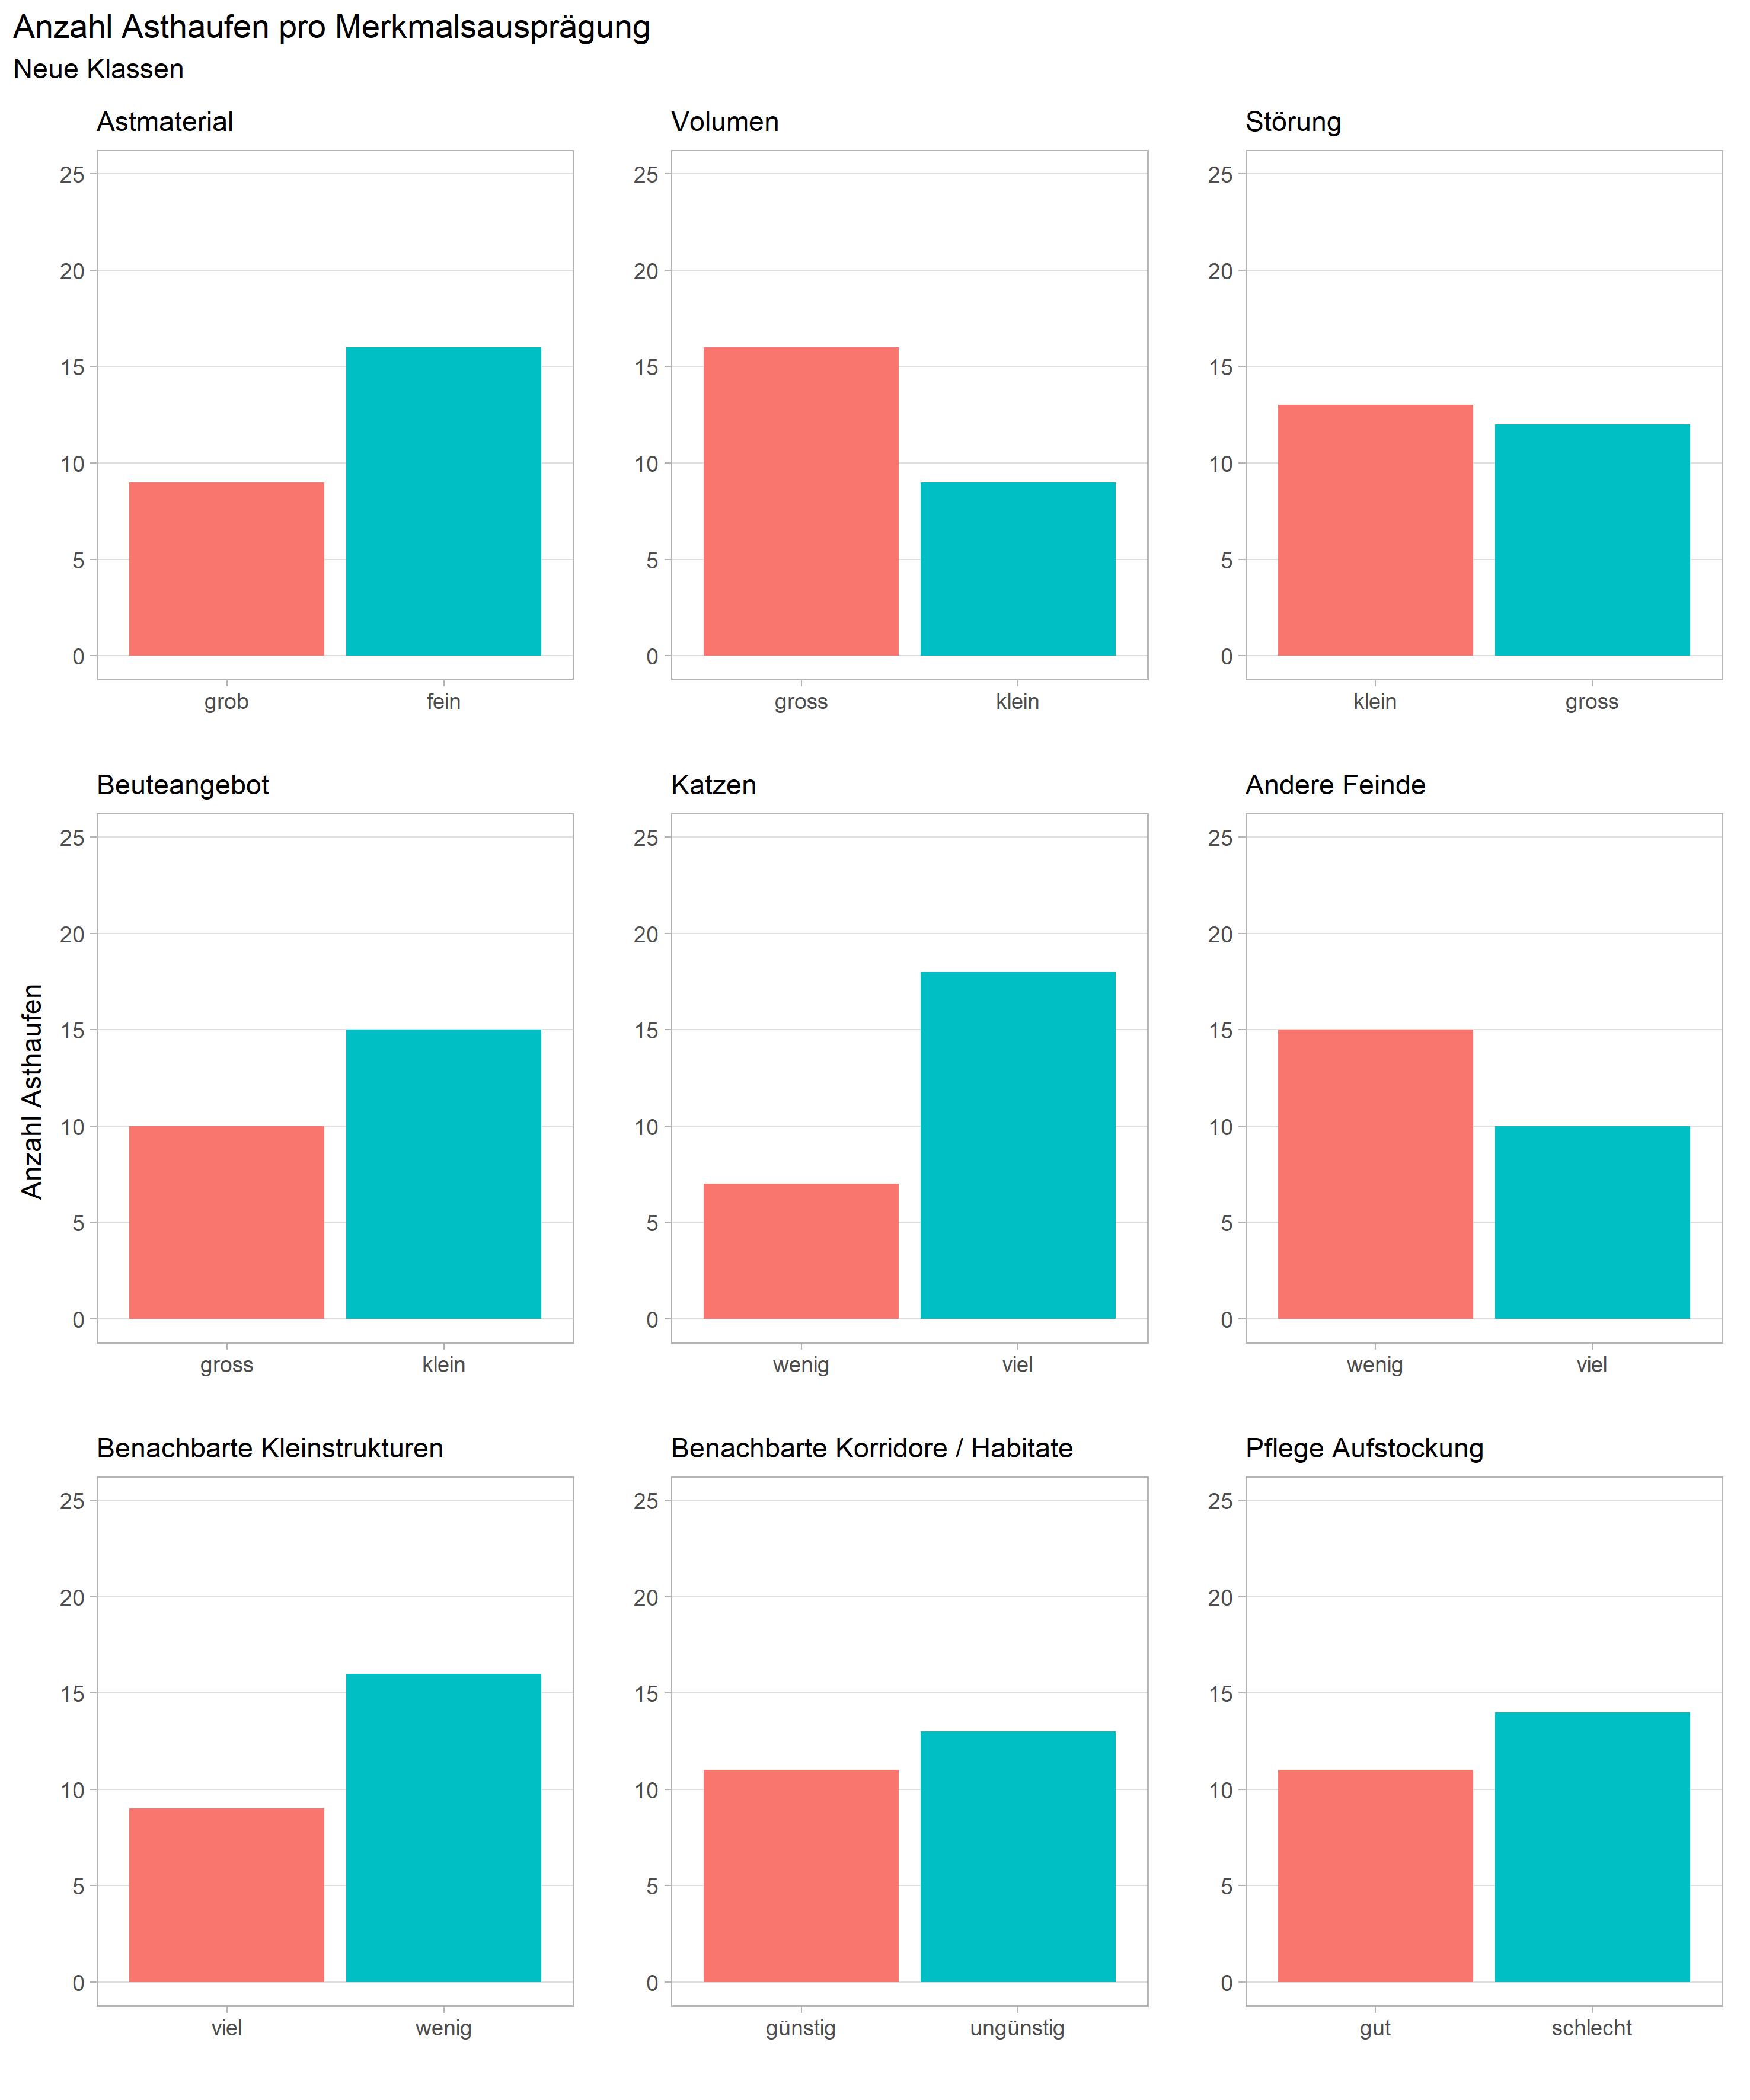
\includegraphics[width=41in]{images/asthaufen_qualitaet_histogramm_newclasses}

\end{document}
